
\clearpage
\section{Plans}
\label{sec:projects-feature-plans}

A plan brings together the intended result, accountable target, and working period. Its type and framework determine which sections you need to complete, so begin with the result you want.

\begin{rcnote}[Example: Horizon]
Sarah creates “Improve Aleppo branch readiness” and selects the target responsible for visits. Defining an owner and period helps her review work with Omar before the visit.
\end{rcnote}

\textbf{Where and who:} Open the “Projects” app, then its “Plans” card. This is a main app page. The person responsible for this work uses it; employees edit only the information their permissions allow.

\subsection{Choose the plan before filling its details}
Start with “Plan Category”, then “Plan Type”, “Primary Target”, and “Base Framework”. “Target Class” is derived from the selected target. Complete the name, accountable owner, dates, and priority; the selected type may require more information, such as a mandate or budget constraint.

Not every tab appears in every plan. Type, framework, overlay frameworks, and lifecycle stage control available sections and editing. If a section is missing, review these choices before creating a replacement record.
\begin{figure}[H]
\centering
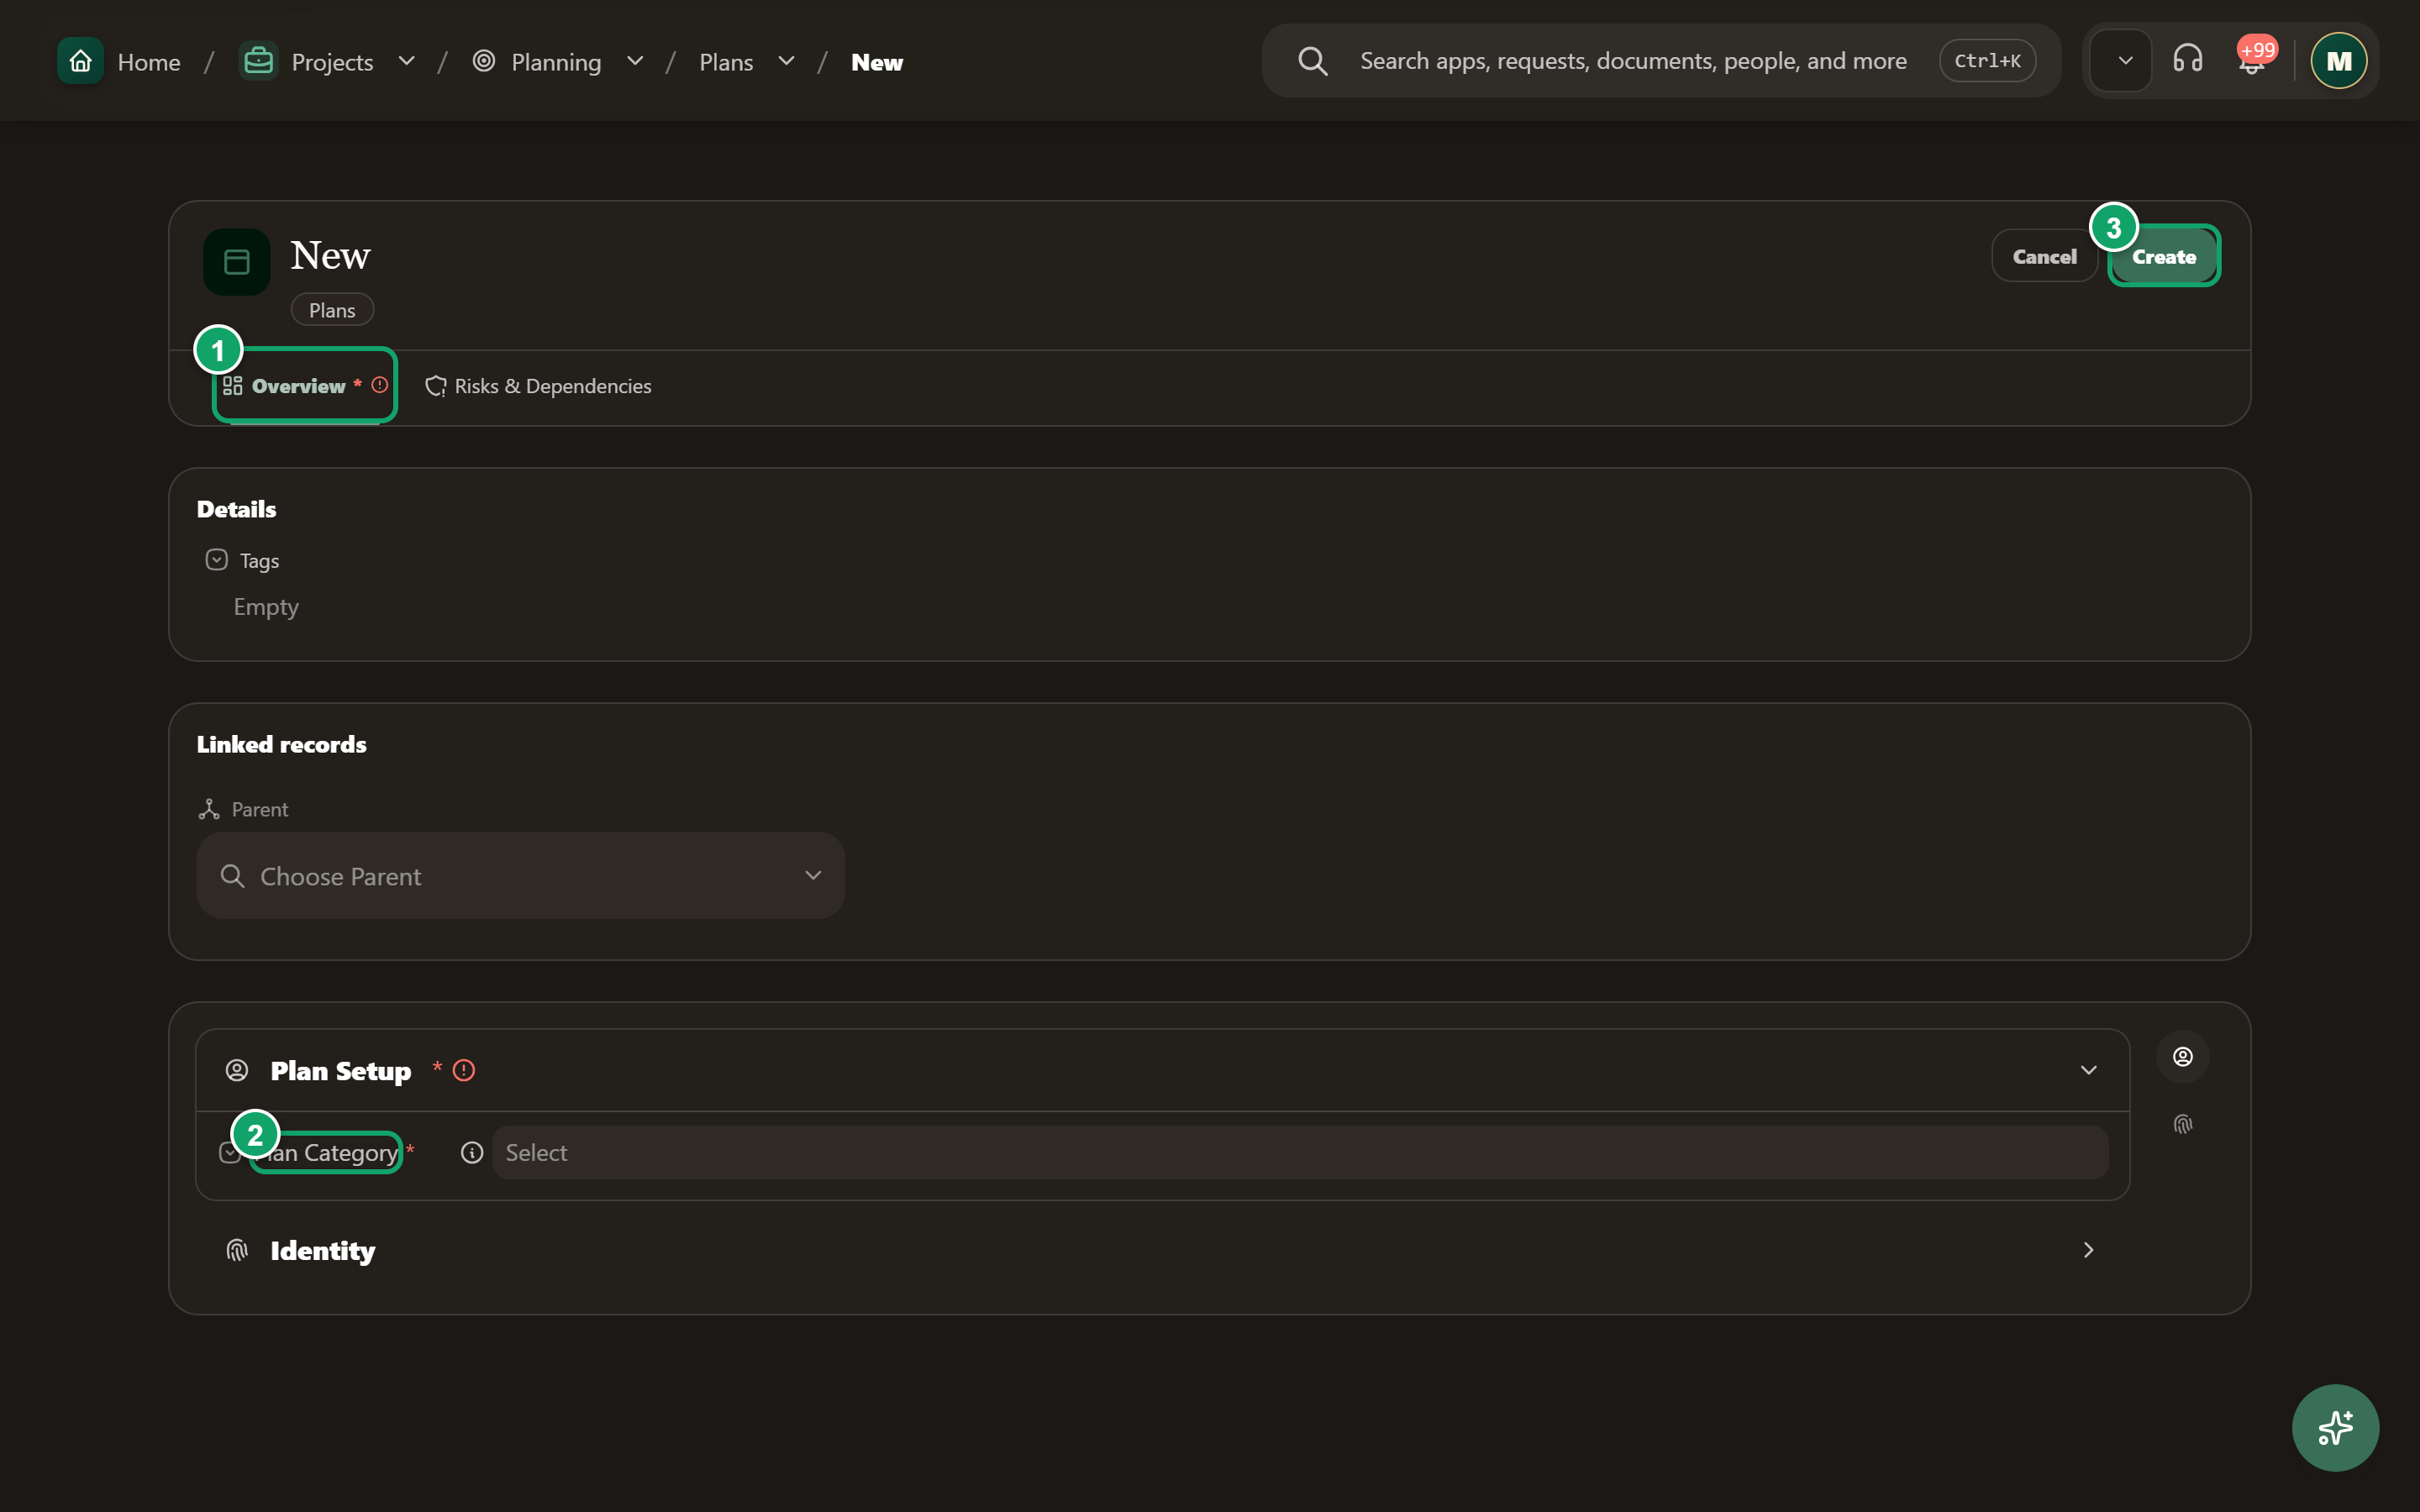
\includegraphics[width=0.95\linewidth,height=0.72\textheight,keepaspectratio]{figures/screens/ch05-plans-en.png}
\caption{Starting a plan before choosing its category}
\label{fig:projects-screen-plans}
\shotnote{The form begins with “Plan Category”, then reveals choices appropriate to that category. Do not expect every field or tab before defining what you are planning; this is an unsaved form. ① The “Overview” tab where the plan starts. ② “Plan Category”: the first required field, which decides the fields that follow. ③ “Create”: saves the plan once the required fields are complete.}
\end{figure}
\begin{table}[H]
\centering
\caption{What do you record?}
\label{tab:projects-plans-fields}
\begin{tabularx}{\linewidth}{R{4.2cm} Y}
\rcHeaderRow
\thh{Information} & \thh{Fields}\\
Required information & “Plan Category”.\\
Required when applicable & “Plan Type”, “Primary Target”, “Base Framework”, “Name”, “Priority”, “Start Date”, “End Date”, “Accountable Owner”, “Action Source Profile”, “Budget Constraint Type”, “Budget Envelope Amount”, “Budget Envelope Currency”, “Mandatory Budget Link”, “Mandate”, “Service / Workload Logic”, “Workload Planning Method”, “Effective Date”, “Jurisdiction / Coverage”, “Policy Type”, “Enforcement Level”. Visibility depends on the record type and configuration.\\
Additional information & “Overlay Frameworks”, “Status”, “Description”, “Planning Horizon”, “Review Cadence”, “Informed”, “Sponsor”, “Governance Body”, “Accountable Unit”, “Review Owner”, “Coverage Nodes”, “Coverage Locations”, “Plan Cycle”, “Scope Targets”, “Upstream Plan”, “Linked Objective”, “Linked Initiative”, “Fiscal Year”, “Forecast Status”, “Success Criteria”, “Expiry Date”, “Supersedes Plan”, “Effectiveness Criteria”, “Planning Notes”, “Tags”.\\
Calculated results & “Target Class”, “Health Status”, “Baseline Summary”, “Baseline Version”, “Version”, “Review State”, “Approval Required”, “Approval Stage”, “Approval State”, “Last Review At”, “Next Review At”, “Rebaseline Flag”, “Rebaseline Reason”, “Planned Resource Effort (hours)”, “Actual Resource Effort (hours)”, “Planned Resource Cost Summary”, “Planned Resource Capacity (hours)”, “Planned Resource Cost”, “Committed Resource Cost”, “Actual Resource Cost Summary”, “Actual Resource Cost”, “Resource Cost Variance”, “Resource Quantity Summary”, “Planned Resource Quantity”, “Actual Resource Quantity”, “Resource Capacity Utilization \%”, “Open Risk Count”, “Blocked Dependency Count”, “Mitigation Coverage \%”, “Inherent Exposure”, “Residual Exposure”, “Scenario Coverage \%”, “BIA Completion \%”, “Procedure Readiness \%”, “Exercise Pass Rate \%”, “Control Coverage \%”, “Open Finding Count”, “Active Incident Count”, “Progress \%”, “Plan Status Stage”, “Plan Profile Key”, “Plan Status Template”. Review the source values if a result differs from expectations.\\
\end{tabularx}
\end{table}
\begin{table}[H]
\centering
\caption{Tabs and related records}
\label{tab:projects-plans-tabs}
\begin{tabularx}{\linewidth}{R{4.2cm} Y}
\rcHeaderRow
\thh{Tab} & \thh{What it contains}\\
“Overview” & “Plan Setup”; “Identity”; “Ownership \& Accountability”; “Governance”; “Timeline”; “Budget Envelope”; “Mandate \& Workload”\\
“Source” & “Action Source \& Alignment”\\
“Milestones” & Shows information for this aspect when the record configuration applies.\\
“Execution” & “Execution Register”; “Work Packages”; “Work Package Paths”; “Deliverables”; “Milestone Model”; “Milestone Register”; “Issues \& Blockers”; “Escalations”; “Service Commitments”; “Service Measurements”; “Service Breaches”; “Recovery Actions”; “Change Requests”; “Gate Reviews”; Planning Milestones (\ref{sec:projects-feature-planning-milestones}); WBS / Work Packages (\ref{sec:projects-feature-wbs-items}); Deliverables / Products (\ref{sec:projects-feature-deliverables})\\
“Alignment” & “Hierarchy \& Alignment Links”\\
“Coverage” & “Coverage”\\
“Scope” & “Primary Target”; “Extended Scope”\\
“Framework” & “Framework Model”; “Strategic Themes”; “Objectives”; “Scorecard Measures”; “Strategy Map”; “OKR Cycles”; “Key Results”; “Check-in Paths”; “Hoshin Alignment”; “X-Matrix / Catchball”; “Logic Models”; “Change Pathway Elements”; “Result Chain”; “Context / Actors / Causal Path”; “Policy Lifecycle”; “Policy Measures”; “Roadmap Model”; “Roadmap Items”; “Objective Paths”; Planning Themes (\ref{sec:projects-feature-planning-themes}); Planning Objectives (\ref{sec:projects-feature-planning-objectives}); OKR Cycles (\ref{sec:projects-feature-planning-okrs}); Key Results (\ref{sec:projects-feature-planning-key-results}); Key Result Check-ins (\ref{sec:projects-feature-planning-key-result-checkins}); Hoshin Items (\ref{sec:projects-feature-planning-hoshin-items}); Hoshin X-Matrix Links (\ref{sec:projects-feature-planning-hoshin-x-matrix-links}); Hoshin Catchball Exchanges (\ref{sec:projects-feature-planning-hoshin-catchball-exchanges}); Hoshin Countermeasures (\ref{sec:projects-feature-planning-hoshin-countermeasures}); Theory of Change (\ref{sec:projects-feature-theory-of-change}); Results Frameworks (\ref{sec:projects-feature-logframes}); Logframe Goals (\ref{sec:projects-feature-logframe-goals}); Logframe Outcomes (\ref{sec:projects-feature-logframe-outcomes}); Logframe Outputs (\ref{sec:projects-feature-logframe-outputs}); Logframe Activities (\ref{sec:projects-feature-logframe-activities})\\
“Initiatives” & “Native Initiatives”; Planning Initiatives (\ref{sec:projects-feature-planning-initiatives})\\
“Deliverables” & Shows information for this aspect when the record configuration applies.\\
“Governance” & “Lifecycle Approvals”; “Review Schedule”; “Governance Reviews”; “Decisions”; “Change History”; “Versions \& Baselines”; Planning Reviews (\ref{sec:projects-feature-planning-reviews}); Planning Approvals (\ref{sec:projects-feature-planning-approvals}); Planning Decisions (\ref{sec:projects-feature-planning-decisions})\\
“Budget” & “Budget Model”; “Budgets”; “Budget Lines”; “Budget Periods”; Budgets (\ref{sec:projects-feature-budgets}); Budget Lines (\ref{sec:projects-feature-budget-lines}); Budget Line Periods (\ref{sec:projects-feature-budget-line-periods})\\
“Funding” & “Funding Model”; “Funding Sources”; Funding Sources (\ref{sec:projects-feature-funding-sources})\\
“Workforce” & “Workforce Model”; “Staffing Demands”; “Positions”; “Assignments”\\
“Hiring” & “Hiring Model”; “Vacancies”\\
“Procurement” & “Procurement Model”; “Procurements”; Procurements (\ref{sec:projects-feature-procurements})\\
“Contracts” & “Contract Model”\\
“Demand \& Capacity” & “Demand \& Capacity Model”\\
“Allocations” & “Allocation Model”; “Capacity Allocations”\\
“Pipeline” & “Fundraising Pipeline”; “Opportunities”\\
“Awards” & “Awards \& Restrictions”\\
“Assets” & “Asset Register Model”; “Asset Register”\\
“Lifecycle” & “Lifecycle Model”; “Lifecycle Events”\\
“Gates” & Shows information for this aspect when the record configuration applies.\\
“Escalations” & Shows information for this aspect when the record configuration applies.\\
“Change Control” & Shows information for this aspect when the record configuration applies.\\
“Resources” & “Resource Model”; “Resources Register”; Planning Resources (\ref{sec:projects-feature-planning-resources}); Resource Allocations (\ref{sec:projects-feature-resource-allocations})\\
“Risks \& Dependencies” & “Risk Model”; “Risks”; “Dependencies”; Planning Dependencies (\ref{sec:projects-feature-planning-dependencies}); Risk Register (\ref{sec:projects-feature-planning-risks})\\
“Performance” & “Performance Model”; “Time-Phased Targets”; “Indicators”; “Indicator Measurements”; “Measurement Paths”; Performance Indicators (\ref{sec:projects-feature-performance-indicators}); Time-Phased Targets (\ref{sec:projects-feature-planning-time-targets})\\
“Data” & “Data Sources”; “Indicator Protocols”; “Reporting Periods”; “Data Quality Reviews”; “Evidence Register”; Reporting Periods (\ref{sec:projects-feature-planning-reporting-periods}); Planning Data Sources (\ref{sec:projects-feature-planning-data-sources}); Evidence Items (\ref{sec:projects-feature-planning-evidence-items})\\
“Evaluation” & “Evaluation Questions”; “Evaluation Findings”; “Management Responses”; Evaluation Questions (\ref{sec:projects-feature-planning-evaluation-questions}); Evaluation Findings (\ref{sec:projects-feature-planning-evaluation-findings}); Management Responses (\ref{sec:projects-feature-planning-management-responses})\\
“Learning” & “Learning Agenda”; “Learning Insights”; Learning Agenda Items (\ref{sec:projects-feature-planning-learning-agenda-items}); Learning Insights (\ref{sec:projects-feature-planning-learning-insights})\\
“Improvement” & “Improvement Opportunities”; Improvement Opportunities (\ref{sec:projects-feature-planning-improvement-opportunities})\\
“Assumptions” & “Assumptions”; “Assumptions Register”; Planning Assumptions (\ref{sec:projects-feature-planning-assumptions})\\
“Cycle” & “Cycle Model”\\
“Consultation” & “Consultation Register”\\
“Publishing” & “Releases”\\
“Commitments” & Shows information for this aspect when the record configuration applies.\\
“Measurements” & Shows information for this aspect when the record configuration applies.\\
“Breaches” & Shows information for this aspect when the record configuration applies.\\
“Recovery” & “Recovery Objectives”; “Recovery Scope”; “Restore \& Failover Sequence”\\
“Controls” & “Control Model”; “Controls Register”; Planning Controls (\ref{sec:projects-feature-planning-controls})\\
“Assessments” & “Control Assessments”; Control Assessments (\ref{sec:projects-feature-planning-control-assessments})\\
“Findings” & “Findings Register”; “Attestations \& Sign-Offs”; Planning Findings (\ref{sec:projects-feature-planning-findings})\\
“Incidents” & “Incident Register”; “Severity \& Classification”; Planning Incidents (\ref{sec:projects-feature-planning-incidents})\\
“Timeline” & “Incident Timeline”; Incident Timeline Events (\ref{sec:projects-feature-planning-incident-events})\\
“Post-Incident” & “Post-Incident Review”\\
“Scenarios” & “Scenario Catalog”; “Trigger Matrix”; “Activation Criteria”; Planning Scenarios (\ref{sec:projects-feature-planning-scenarios})\\
“Playbooks” & “Playbook Model”\\
“BIA” & “BIA Model”; “BIA Register”; BIA Entries (\ref{sec:projects-feature-planning-bia-entries})\\
“Continuity” & “Continuity Strategies”; “Manual Workarounds”\\
“Procedures” & “Procedures \& Runbooks”; Planning Procedures (\ref{sec:projects-feature-planning-procedures})\\
“Exercises” & “Exercises \& Tests”; Planning Exercises (\ref{sec:projects-feature-planning-exercises})\\
“Tests” & “Recovery Test Program”\\
\end{tabularx}
\end{table}
\begin{figure}[H]
\centering
\begin{tikzpicture}[node distance=0.5cm]
\node[stepBox] (n0) {Choose work page};
\node[stepBox,below=of n0] (n1) {Plans};
\node[stepBox,below=of n1] (n2) {Save and reopen};
\draw[flowsTo] (n0) -- (n1);
\draw[flowsTo] (n1) -- (n2);
\end{tikzpicture}
\rclegend
\caption{Work and verification path}
\label{fig:projects-plans-flow}
\shotnote{Begin by opening “Plans” and choosing the correct record before entering details. Reopening after saving checks persistence; it does not imply approval or completion of related work.}
\end{figure}

\subsection{Actions and verification}
\begin{enumerate}
\item Open “Plans” in Projects, then select “Add”. Choose “Plan Category” first, followed by an available plan type matching the intended work.
\item Choose “Primary Target” from available records, then “Base Framework”. Complete the name, accountable owner, priority, and start and end dates, and review any additional fields required by that type.
\item Select “Create”, then reopen the plan. Check its target, owner, and period, and use the available sections to add objectives, delivery, or measurement as appropriate.
\item Check the plan stage before editing; it may restrict configuration changes or related records. Resolve validation or ask for an access review rather than duplicating the plan.
\end{enumerate}

\textbf{Try the example:} In the fictional example, use “Aleppo branch readiness plan” for “Name”, then complete the other information to suit Horizon's work. Example values do not replace the actual records required by relation fields.

\textbf{Check and recover:} The record should be present when reopened, with its saved values. If it is missing, check search, filters, scope, and access before creating another. If saving fails, resolve required fields and validation messages; missing tabs or locked fields require checking record type, framework, and stage with the responsible person.

\clearpage
\section{Projects}
\label{sec:projects-feature-projects}

A project organizes a defined scope of work with a manager and an intended result. Begin with its definition and charter, then use the available sections to plan delivery and review progress.

\begin{rcnote}[Example: Horizon]
Sarah creates “Prepare the Aleppo branch visit” with code \en{HZN-PRJ-01} and defines its intended result in the charter. Omar prepares the visit pack once assigned, and Sarah reviews the deliverable at handover.
\end{rcnote}

\textbf{Where and who:} Open the “Projects” app, then its “Projects” card. This is a main app page. The person responsible for this work uses it; employees edit only the information their permissions allow.

\subsection{The charter precedes detailed planning}
The “Charter” tab brings together purpose, objectives, success criteria, scope and exclusions, business case, assumptions, risks, and approval details. Review “Project Manager”, “Sponsor”, and dates; saving the record does not approve its charter.

Planning sections require an approved “Charter Status” and a project beyond setup. “Framework” and “Delivery Approach” determine available phases, sprints, and governance, while project and client types affect procurement and monitoring. Setup fields may lock after approval; subsequent changes are reviewed through change control.

\textbf{Progress and health:} Progress is calculated from relevant delivery records. Review work packages, deliverables, and indicators before interpreting project health; completion of one task does not mean the whole project is complete.
\begin{figure}[H]
\centering
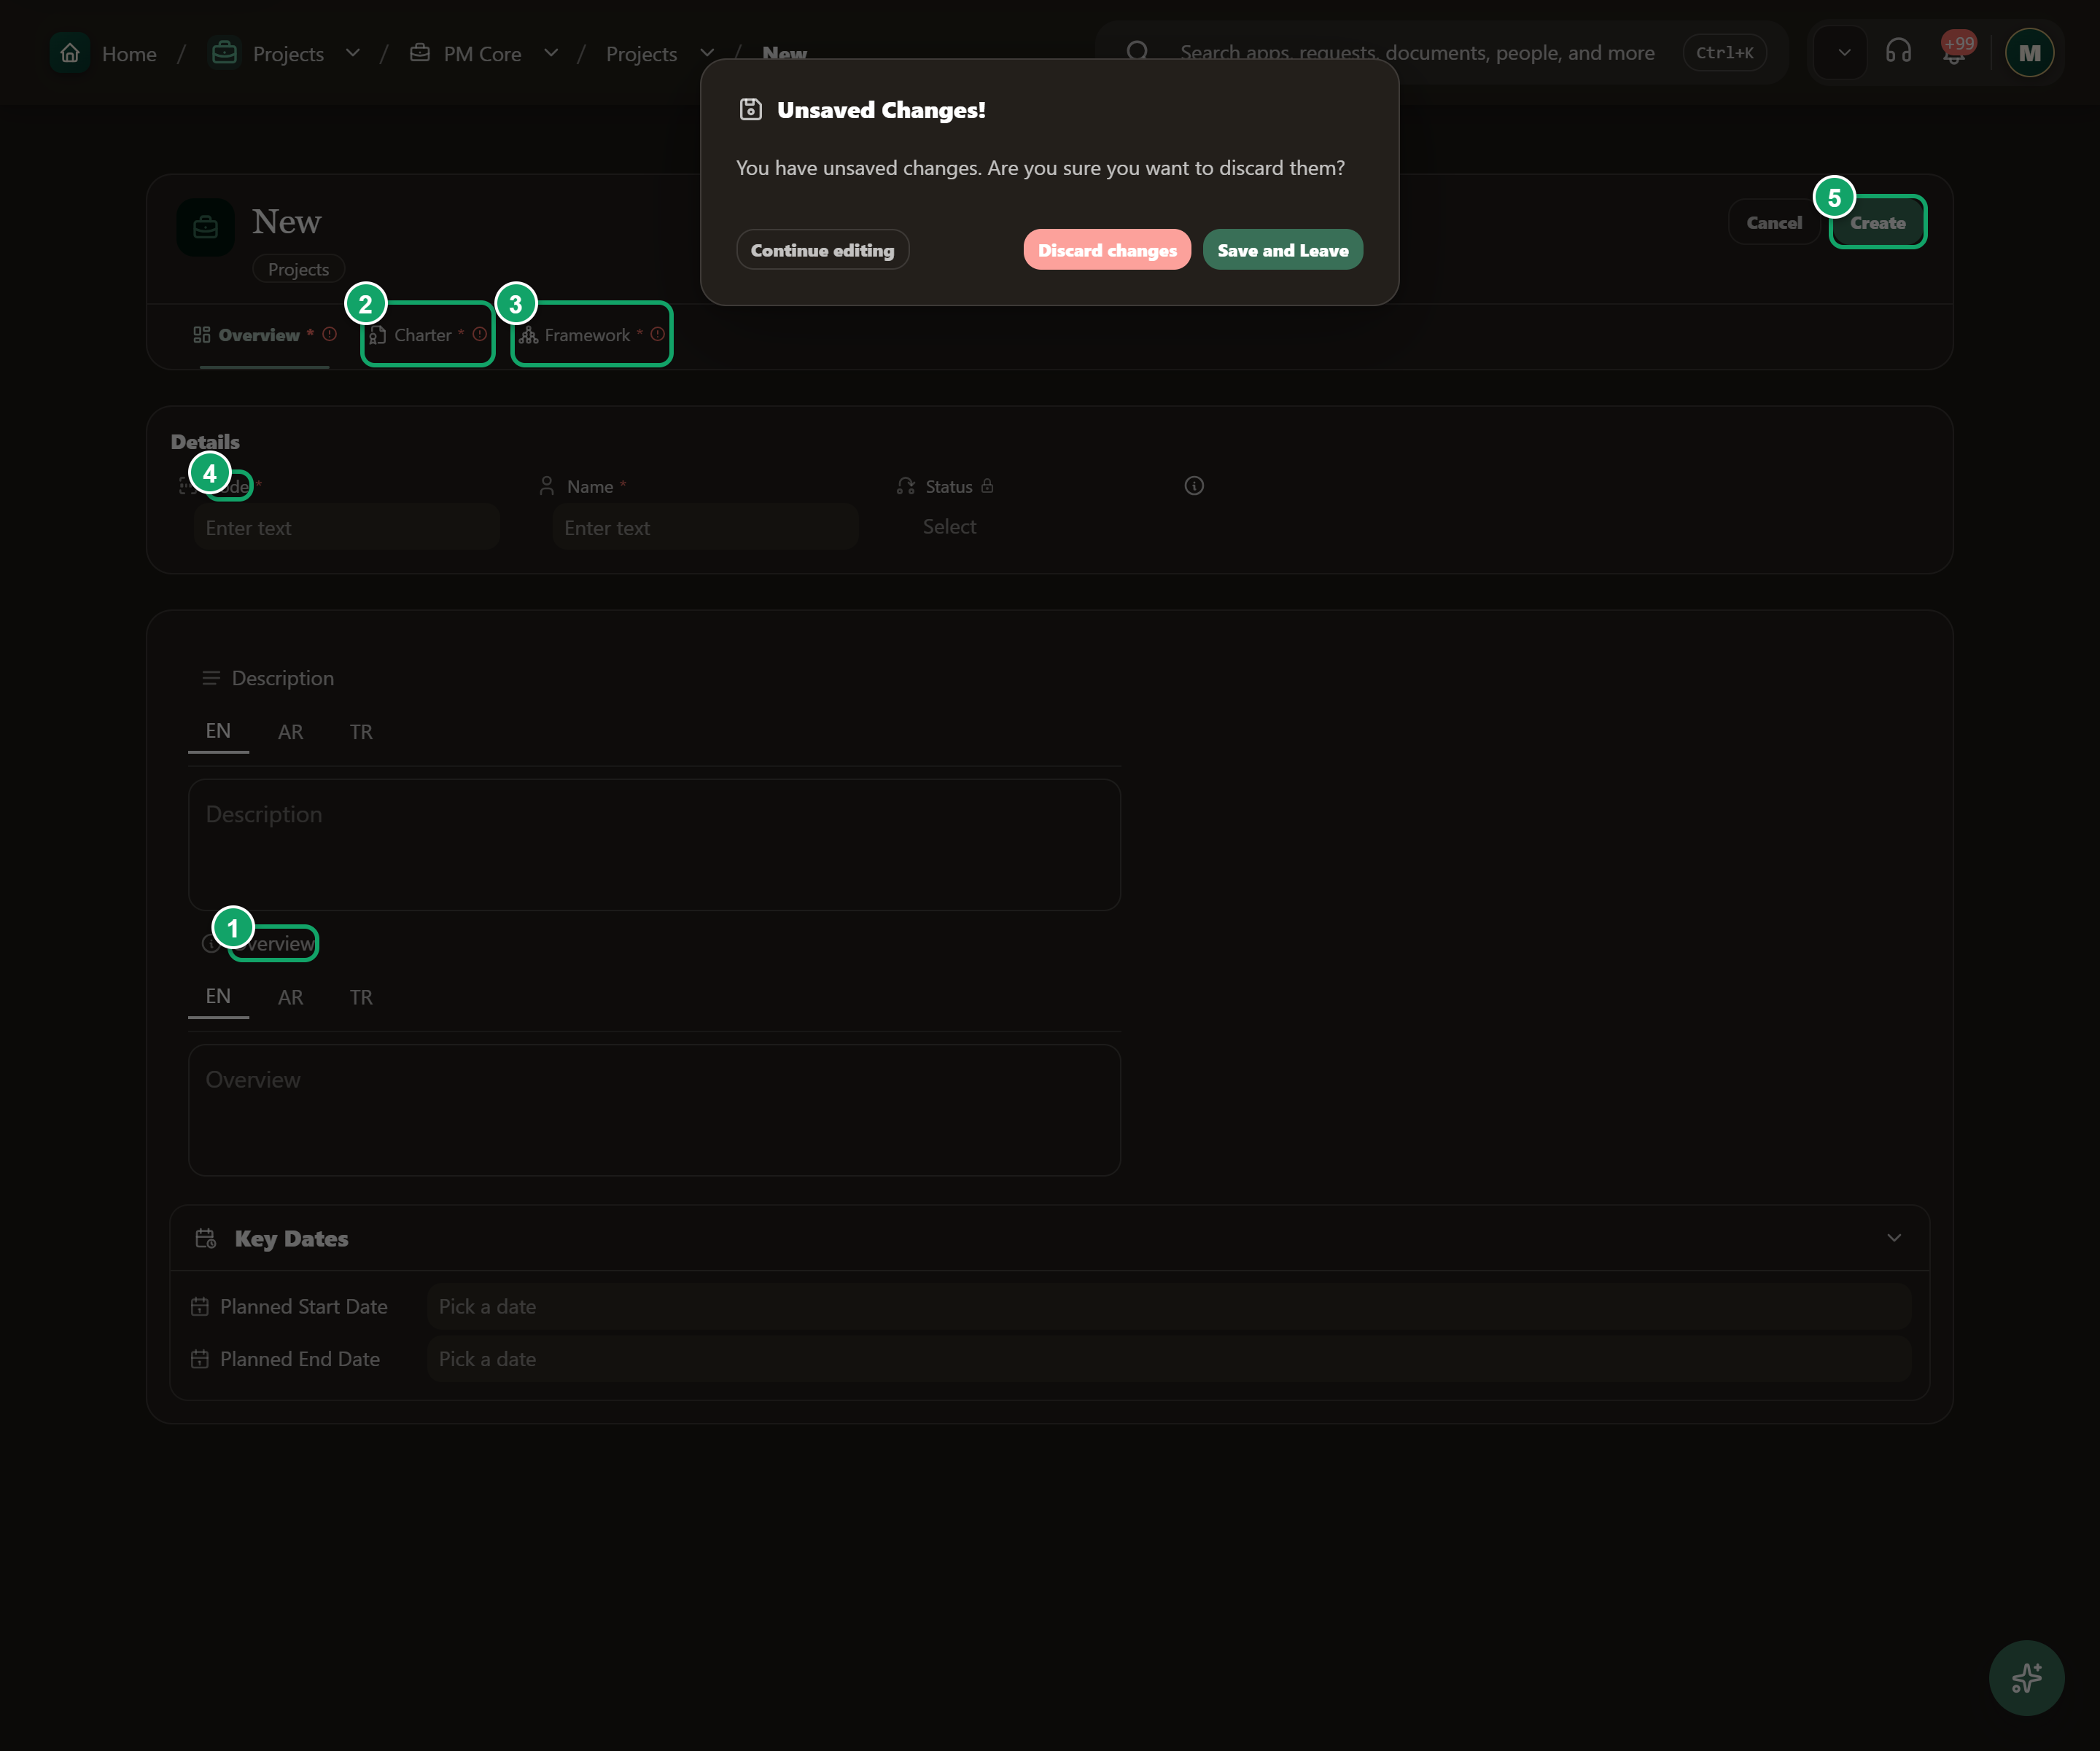
\includegraphics[width=0.95\linewidth,height=0.72\textheight,keepaspectratio]{figures/screens/ch05-project-create-en.png}
\caption{Overview of an unsaved new project}
\label{fig:projects-screen-project-create}
\shotnote{This tab collects project identity, description, and planned dates. Name and code alone do not complete creation: the other tabs require charter and framework information, and project status depends on configuration. ① The “Overview” tab. ② The “Charter” tab. ③ The “Framework” tab; the red mark means the tab has an empty required field. ④ “Code”: the first required field. ⑤ “Create”.}
\end{figure}
\begin{figure}[H]
\centering
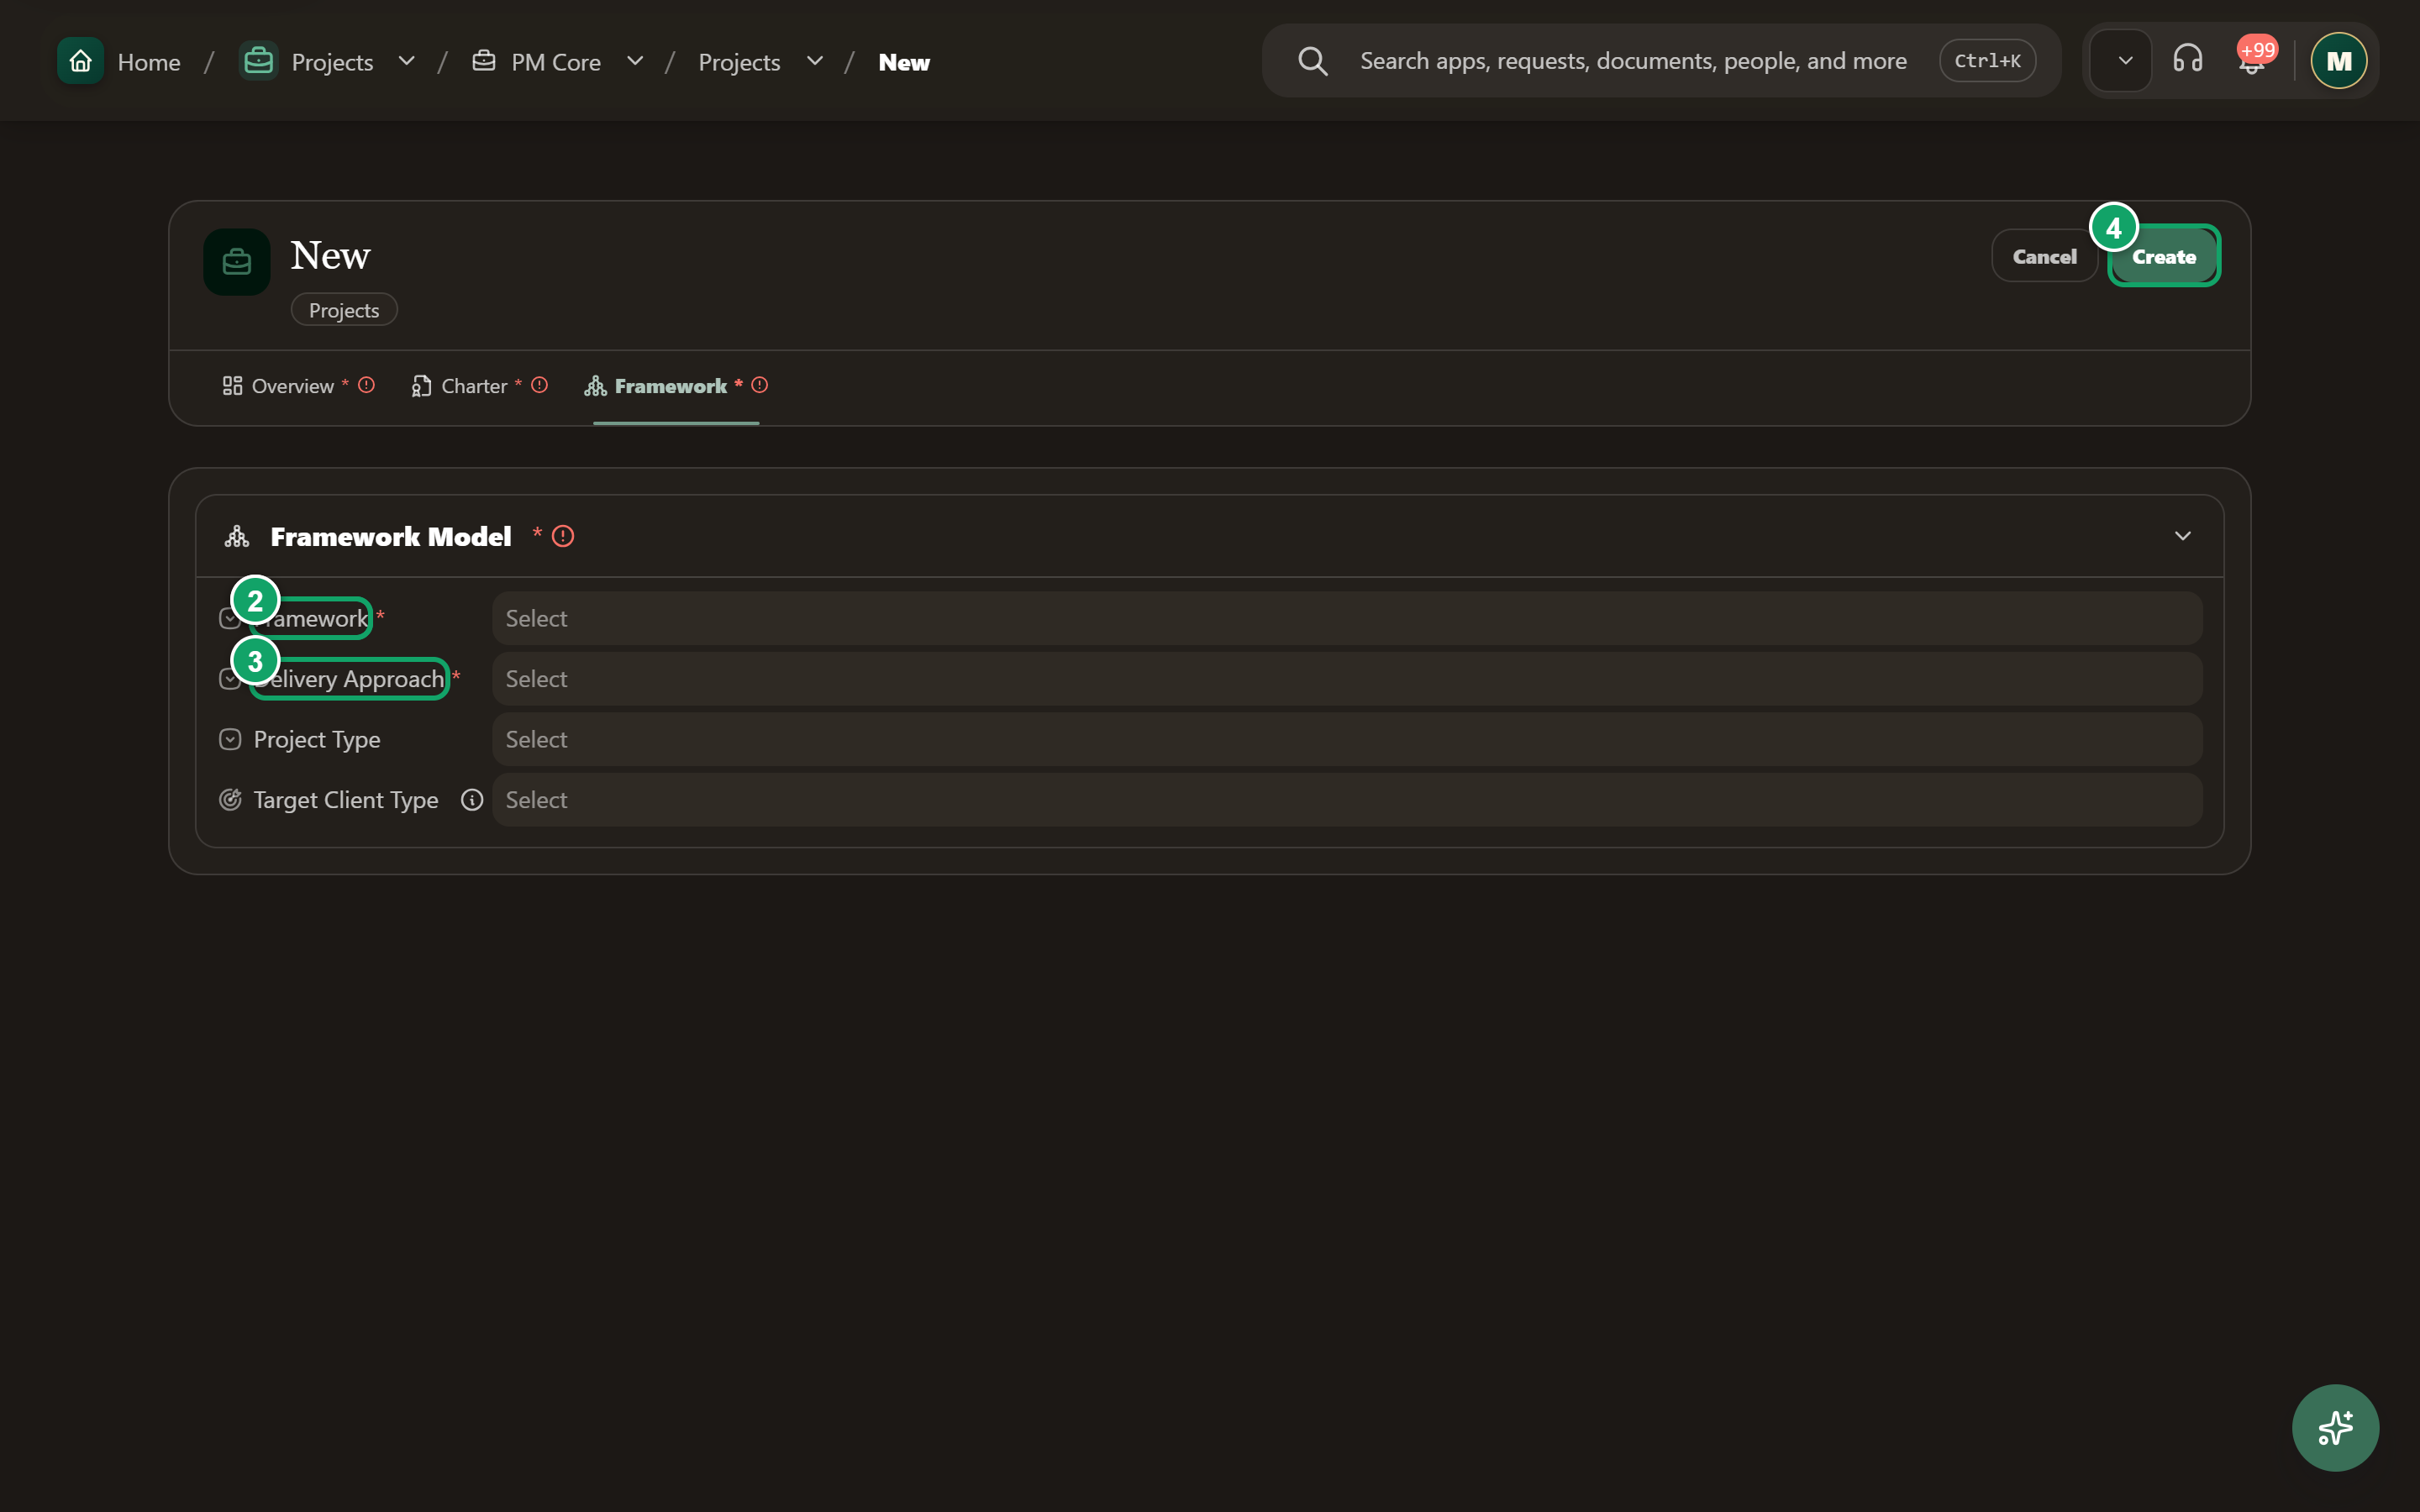
\includegraphics[width=0.95\linewidth,height=0.72\textheight,keepaspectratio]{figures/screens/ch05-project-framework-en.png}
\caption{Choosing the project framework and delivery approach}
\label{fig:projects-screen-project-framework}
\shotnote{“Framework” and “Delivery Approach” determine how the project is organized and which sections apply. Review project and target client types too, as they help determine procurement and monitoring needs; the pictured form is unsaved. ① The “Framework” tab. ② “Framework”: the method used to run the project. ③ “Delivery Approach”: how results are delivered. ④ “Create”: saves the project once the required tabs are complete.}
\end{figure}
\begin{figure}[H]
\centering
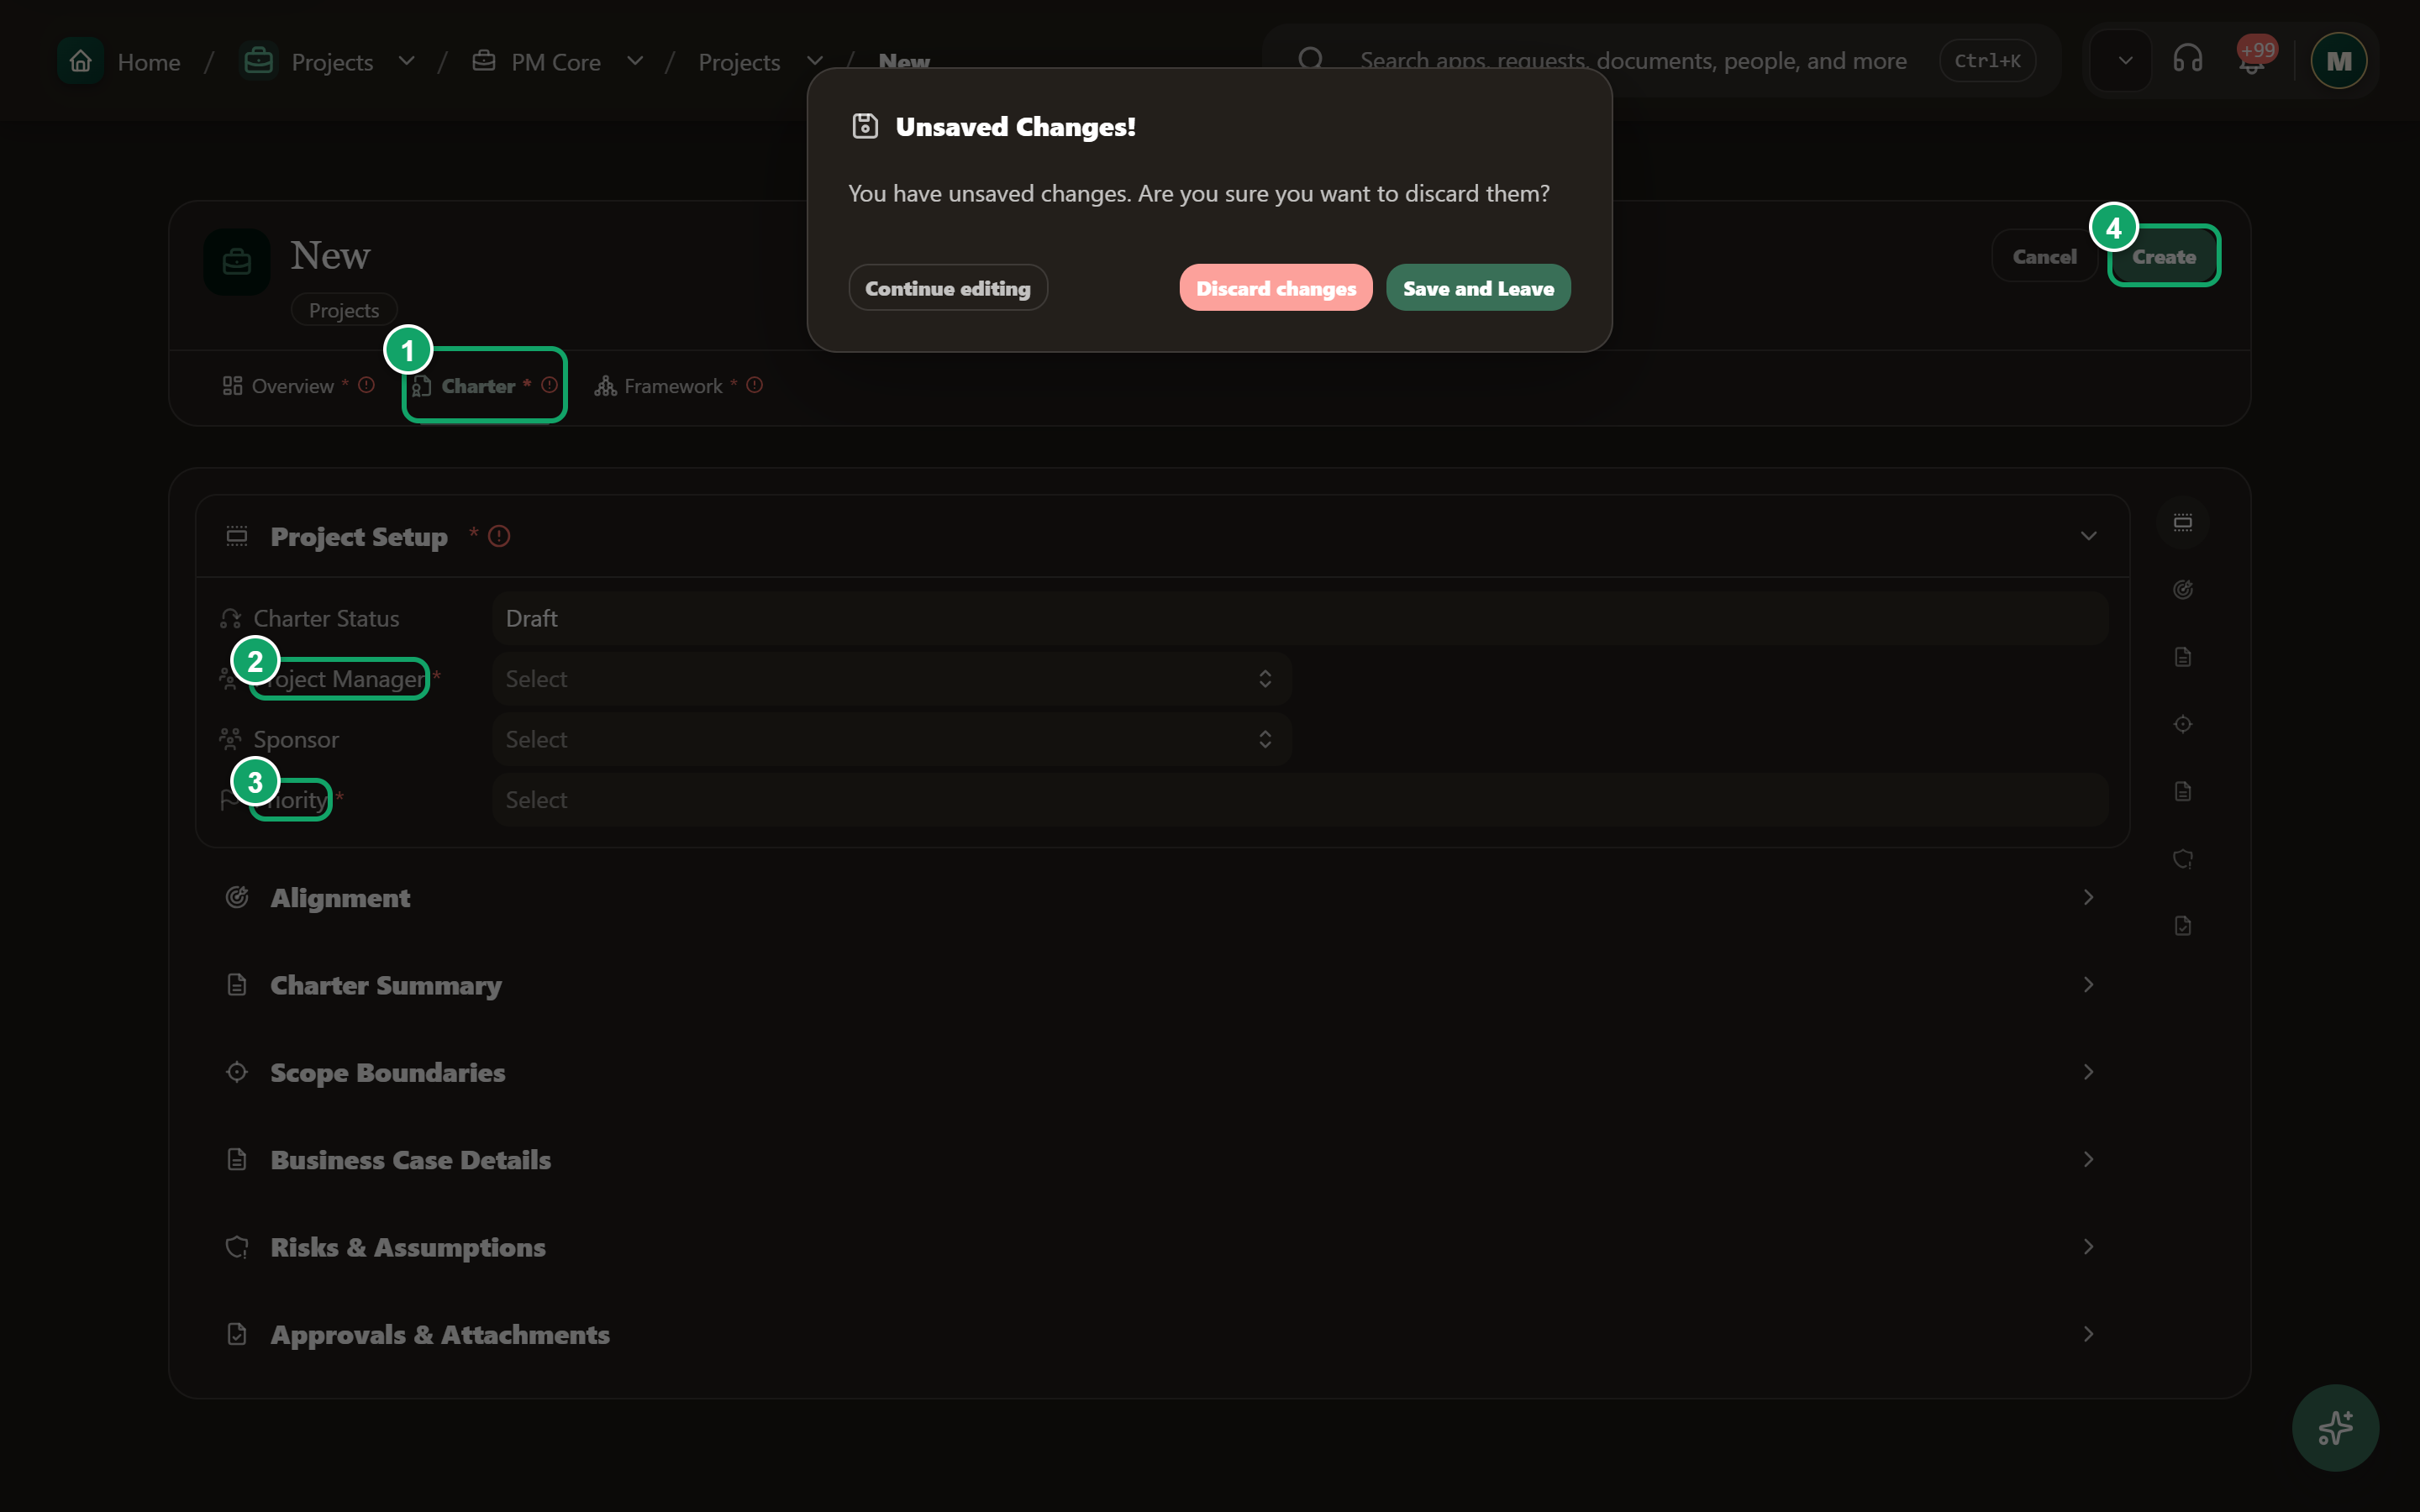
\includegraphics[width=0.95\linewidth,height=0.72\textheight,keepaspectratio]{figures/screens/ch05-project-charter-en.png}
\caption{Project setup and charter sections}
\label{fig:projects-screen-project-charter}
\shotnote{The charter is in “Draft”, with project manager, sponsor, and priority selections. The remaining sections cover purpose, scope, business case, risks, and approval; opening this tab or saving its fields does not mean the charter has been approved. ① The “Charter” tab. ② “Project Manager”. ③ “Priority”. ④ “Create”.}
\end{figure}
\begin{table}[H]
\centering
\caption{What do you record?}
\label{tab:projects-projects-fields}
\begin{tabularx}{\linewidth}{R{4.2cm} Y}
\rcHeaderRow
\thh{Information} & \thh{Fields}\\
Required information & “Code”, “Name”, “Framework”, “Delivery Approach”, “Project Manager”, “Priority”.\\
Additional information & “Description”, “Project Type”, “Target Client Type”, “Status”, “Charter Status”, “Charter Title”, “Purpose”, “Objectives”, “Success Criteria”, “Scope Description”, “Out of Scope”, “Business Case Type”, “Strategic Alignment”, “Expected Benefits”, “Stakeholder Impact”, “Expected ROI”, “Estimated Budget”, “Estimated Duration (days)”, “Target Start Date”, “Target End Date”, “Key Assumptions”, “Key Constraints”, “Key Risks”, “Approved By”, “Approval Date”, “Attachments”, “Portfolio”, “Program”, “Plans”, “Sponsor”, “Owners”, “Informed”, “Scope Health Override”, “Quality Health Override”, “Planned Start Date”, “Planned End Date”, “Actual Start Date”, “Actual End Date”, “Current Phase”, “Currency”, “Planned Budget”, “Actual Cost”, “Earned Value (EV)”, “Planned Value (PV)”, “Sector”, “Donors”, “Logical Framework”, “Tags”.\\
Calculated results & “Project Status Template”, “Setup Stage”, “Setup Profile”, “Setup Complete”, “Governance Required”, “Overall Health”, “Scope Health”, “Schedule Health”, “Cost Health”, “Quality Health”, “Risk Health”, “Cost Performance Index (CPI)”, “Schedule Performance Index (SPI)”, “Progress \%”. Review the source values if a result differs from expectations.\\
\end{tabularx}
\end{table}
\begin{table}[H]
\centering
\caption{Tabs and related records}
\label{tab:projects-projects-tabs}
\begin{tabularx}{\linewidth}{R{4.2cm} Y}
\rcHeaderRow
\thh{Tab} & \thh{What it contains}\\
“Overview” & “Snapshot”; “Key Dates”\\
“Charter” & “Project Setup”; “Alignment”; “Charter Summary”; “Scope Boundaries”; “Business Case Details”; “Risks \& Assumptions”; “Approvals \& Attachments”\\
“Framework” & “Framework Model”; Planning Themes (\ref{sec:projects-feature-planning-themes}); Planning Objectives (\ref{sec:projects-feature-planning-objectives}); OKR Cycles (\ref{sec:projects-feature-planning-okrs}); Key Results (\ref{sec:projects-feature-planning-key-results}); Key Result Check-ins (\ref{sec:projects-feature-planning-key-result-checkins}); Hoshin Items (\ref{sec:projects-feature-planning-hoshin-items}); Hoshin X-Matrix Links (\ref{sec:projects-feature-planning-hoshin-x-matrix-links}); Hoshin Catchball Exchanges (\ref{sec:projects-feature-planning-hoshin-catchball-exchanges}); Hoshin Countermeasures (\ref{sec:projects-feature-planning-hoshin-countermeasures}); Theory of Change (\ref{sec:projects-feature-theory-of-change}); Results Frameworks (\ref{sec:projects-feature-logframes}); Logframe Goals (\ref{sec:projects-feature-logframe-goals}); Logframe Outcomes (\ref{sec:projects-feature-logframe-outcomes}); Logframe Outputs (\ref{sec:projects-feature-logframe-outputs}); Logframe Activities (\ref{sec:projects-feature-logframe-activities})\\
“Execution” & “Scope/WBS \& Work Packages”; “Deliverables / Products”; “Execution Control”; “Tasks / Activities”; Planning Milestones (\ref{sec:projects-feature-planning-milestones}); WBS / Work Packages (\ref{sec:projects-feature-wbs-items}); Deliverables / Products (\ref{sec:projects-feature-deliverables}); Requirements (\ref{sec:projects-feature-requirements})\\
“Performance” & “Health Indicators”; “Measurement Paths”; “Indicators”; “Measurements”; “Scorecard”; “Data Quality”; “Status Reporting”; “Earned Value”; Status Reports (\ref{sec:projects-feature-status-reports}); Performance Indicators (\ref{sec:projects-feature-performance-indicators}); Time-Phased Targets (\ref{sec:projects-feature-planning-time-targets})\\
“Resources” & “Leadership”; “Ownership \& Communications”; “Core Team”; “Stakeholders”; “RACI Matrix”; Planning Resources (\ref{sec:projects-feature-planning-resources}); Team Roles (\ref{sec:projects-feature-team-roles}); RACI Matrix (\ref{sec:projects-feature-raci-entries}); Resource Allocations (\ref{sec:projects-feature-resource-allocations}); Stakeholders (\ref{sec:projects-feature-stakeholders})\\
“Scope” & Shows information for this aspect when the record configuration applies.\\
“Schedule” & “Current Phase”; Project Phases (\ref{sec:projects-feature-phases}); Dependencies (\ref{sec:projects-feature-dependencies}); Baselines (\ref{sec:projects-feature-baselines})\\
“Financials” & “Budget Summary”; “Cost Tracking”; “Earned Value Management”; Expenditures (\ref{sec:projects-feature-expenditures})\\
“Quality” & Quality Criteria (\ref{sec:projects-feature-quality-criteria})\\
“Risks \& Issues” & Planning Dependencies (\ref{sec:projects-feature-planning-dependencies}); Risk Register (\ref{sec:projects-feature-planning-risks}); PM Risk Register (\ref{sec:projects-feature-project-risks}); Issues (\ref{sec:projects-feature-issues})\\
“Communications” & “Communication Plan”; Communication Plan (\ref{sec:projects-feature-communication-plan})\\
“Procurement” & Procurements (\ref{sec:projects-feature-procurements})\\
“Governance” & “Metadata”; Planning Reviews (\ref{sec:projects-feature-planning-reviews}); Planning Approvals (\ref{sec:projects-feature-planning-approvals}); Planning Decisions (\ref{sec:projects-feature-planning-decisions}); Gate Reviews (\ref{sec:projects-feature-gate-reviews}); Change Requests (\ref{sec:projects-feature-change-requests}); Meeting Decisions (\ref{sec:projects-feature-meeting-decisions}); Lessons Learned (\ref{sec:projects-feature-lessons-learned})\\
“Agile” & Sprints (\ref{sec:projects-feature-sprints}); Definition of Done (\ref{sec:projects-feature-definition-of-done})\\
“Monitoring \& Evaluation” & “Monitoring Setup”; Beneficiaries (\ref{sec:projects-feature-beneficiaries})\\
\end{tabularx}
\end{table}
\begin{figure}[H]
\centering
\begin{tikzpicture}[node distance=0.5cm]
\node[stepBox] (n0) {Choose work page};
\node[stepBox,below=of n0] (n1) {Projects};
\node[stepBox,below=of n1] (n2) {Save and reopen};
\draw[flowsTo] (n0) -- (n1);
\draw[flowsTo] (n1) -- (n2);
\end{tikzpicture}
\rclegend
\caption{Work and verification path}
\label{fig:projects-projects-flow}
\shotnote{Begin by opening “Projects” and choosing the correct record before entering details. Reopening after saving checks persistence; it does not imply approval or completion of related work.}
\end{figure}

\subsection{Actions and verification}
\begin{enumerate}
\item Open “Projects” and select “Add”. In “Overview”, enter the code and name and the planned dates when known.
\item Open “Framework” and choose “Framework” and “Delivery Approach”. Review project and target client types because they affect sections available later.
\item Open “Charter” and choose “Project Manager” and “Priority”. Complete purpose, objectives, scope, and success criteria, and review sponsor and approval details with the project owner.
\item Select “Create” and reopen the project. Check its name, manager, and framework; do not mark the charter approved merely to expose tabs.
\item After review and approval under the organization’s permissions, check setup stage and available tabs. Add appropriate delivery records, then review progress against actual results.
\end{enumerate}

\textbf{Try the example:} In the fictional example, use “Prepare the Aleppo branch visit” for “Name”, then complete the other information to suit Horizon's work. Example values do not replace the actual records required by relation fields.

\textbf{Check and recover:} The record should be present when reopened, with its saved values. If it is missing, check search, filters, scope, and access before creating another. If saving fails, resolve required fields and validation messages; missing tabs or locked fields require checking record type, framework, and stage with the responsible person.

\clearpage
\section{Portfolios}
\label{sec:projects-feature-portfolios}

A portfolio groups programs and projects that serve a common direction and helps management review priorities and funding. Use it when several efforts need oversight together; a portfolio link is not a general prerequisite for creating a project.

\begin{rcnote}[Example: Horizon]
Horizon management groups branch development work in a portfolio and asks Sarah to maintain the Aleppo visit information. Management reviews priorities across linked projects while keeping their records distinct.
\end{rcnote}

\textbf{Where and who:} Open the “Projects” app, then its “Portfolios” card. This is a main app page. The person responsible for this work uses it; employees edit only the information their permissions allow.

\begin{figure}[H]
\centering
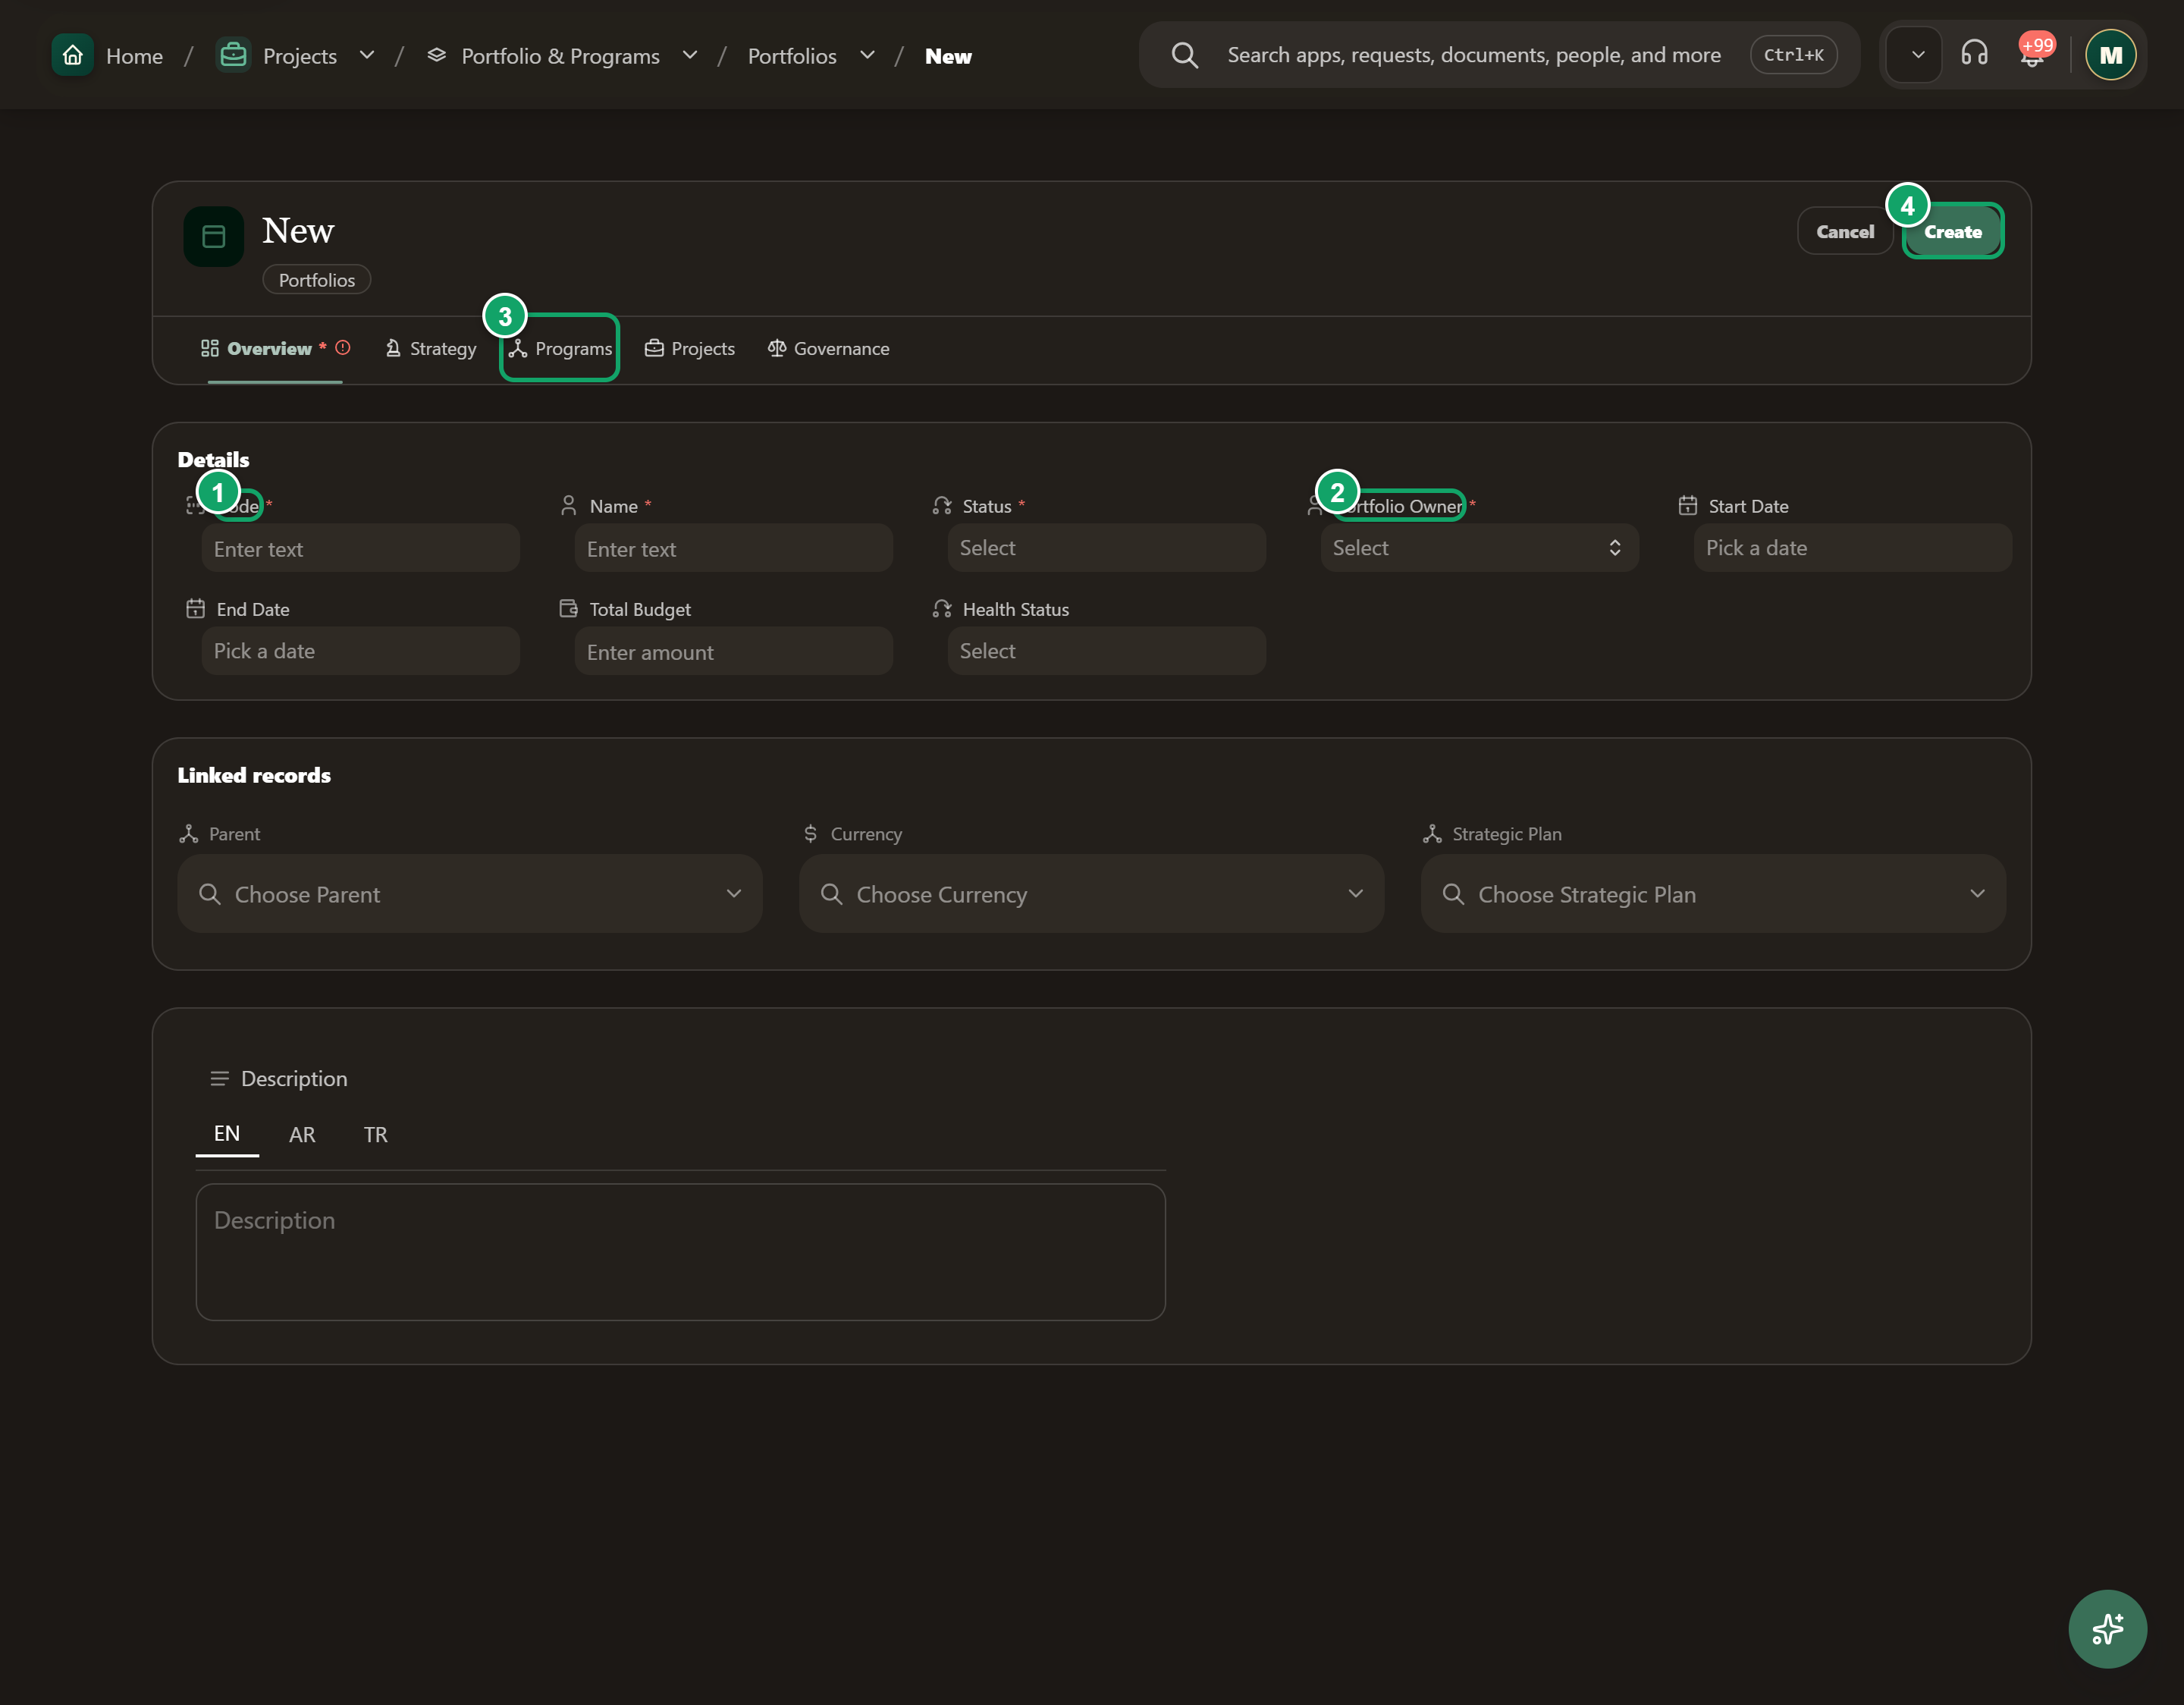
\includegraphics[width=0.95\linewidth,height=0.72\textheight,keepaspectratio]{figures/screens/ch05-portfolios-en.png}
\caption{A new portfolio before saving}
\label{fig:projects-screen-portfolios}
\shotnote{Portfolio information identifies its name, owner, and status before programs and projects are associated with it. Strategic plan and currency appear among related data; creating the portfolio remains separate from creating any programs that may belong to it. ① “Code”: a unique code for the portfolio. ② “Portfolio Owner”. ③ The “Programs” tab gathering the portfolio’s programs. ④ “Create”.}
\end{figure}
\begin{table}[H]
\centering
\caption{What do you record?}
\label{tab:projects-portfolios-fields}
\begin{tabularx}{\linewidth}{R{4.2cm} Y}
\rcHeaderRow
\thh{Information} & \thh{Fields}\\
Required information & “Code”, “Name”, “Status”, “Portfolio Owner”.\\
Additional information & “Description”, “Strategic Alignment”, “Start Date”, “End Date”, “Total Budget”, “Currency”, “Health Status”, “Prioritization Method”, “Maturity Level”, “Strategic Plan”, “Tags”.\\
\end{tabularx}
\end{table}
\begin{table}[H]
\centering
\caption{Tabs and related records}
\label{tab:projects-portfolios-tabs}
\begin{tabularx}{\linewidth}{R{4.2cm} Y}
\rcHeaderRow
\thh{Tab} & \thh{What it contains}\\
“Overview” & “Portfolio Summary”; “Timeline \& Health”\\
“Strategy” & “Strategy Alignment”\\
“Programs” & Programs (\ref{sec:projects-feature-programs})\\
“Projects” & Projects (\ref{sec:projects-feature-projects})\\
“Financials” & Shows information for this aspect when the record configuration applies.\\
“Governance” & “Governance Model”; Planning Reviews (\ref{sec:projects-feature-planning-reviews}); Planning Approvals (\ref{sec:projects-feature-planning-approvals}); Planning Decisions (\ref{sec:projects-feature-planning-decisions})\\
\end{tabularx}
\end{table}
\begin{figure}[H]
\centering
\begin{tikzpicture}[node distance=0.5cm]
\node[stepBox] (n0) {Choose work page};
\node[stepBox,below=of n0] (n1) {Portfolios};
\node[stepBox,below=of n1] (n2) {Save and reopen};
\draw[flowsTo] (n0) -- (n1);
\draw[flowsTo] (n1) -- (n2);
\end{tikzpicture}
\rclegend
\caption{Work and verification path}
\label{fig:projects-portfolios-flow}
\shotnote{Begin by opening “Portfolios” and choosing the correct record before entering details. Reopening after saving checks persistence; it does not imply approval or completion of related work.}
\end{figure}

\subsection{Actions and verification}
\begin{enumerate}
\item Open “Portfolios” and select “Add”. Enter the code and name and choose status and portfolio owner.
\item Complete strategy, dates, and budget information as needed, then select “Create”. A budget amount alone is not evidence of available funding.
\item Reopen the portfolio and check owner and status. To associate a program or project, select this portfolio in that record and confirm it appears among related records.
\end{enumerate}

\textbf{Try the example:} In the fictional example, use “Horizon branch development” for “Name”, then complete the other information to suit Horizon's work. Example values do not replace the actual records required by relation fields.

\textbf{Check and recover:} The record should be present when reopened, with its saved values. If it is missing, check search, filters, scope, and access before creating another. If saving fails, resolve required fields and validation messages; missing tabs or locked fields require checking record type, framework, and stage with the responsible person.

\clearpage
\section{Programs}
\label{sec:projects-feature-programs}

A program coordinates related projects to achieve a shared benefit. Its manager reviews projects, outcomes, and resources together; the program can optionally belong to a portfolio.

\begin{rcnote}[Example: Horizon]
Sarah links the Aleppo visit project to “Branch service improvement” after agreeing with its manager. It appears among the program’s projects so its benefit can be reviewed alongside related work.
\end{rcnote}

\textbf{Where and who:} Open the “Projects” app, then its “Programs” card. This is a main app page. The person responsible for this work uses it; employees edit only the information their permissions allow.

\begin{figure}[H]
\centering
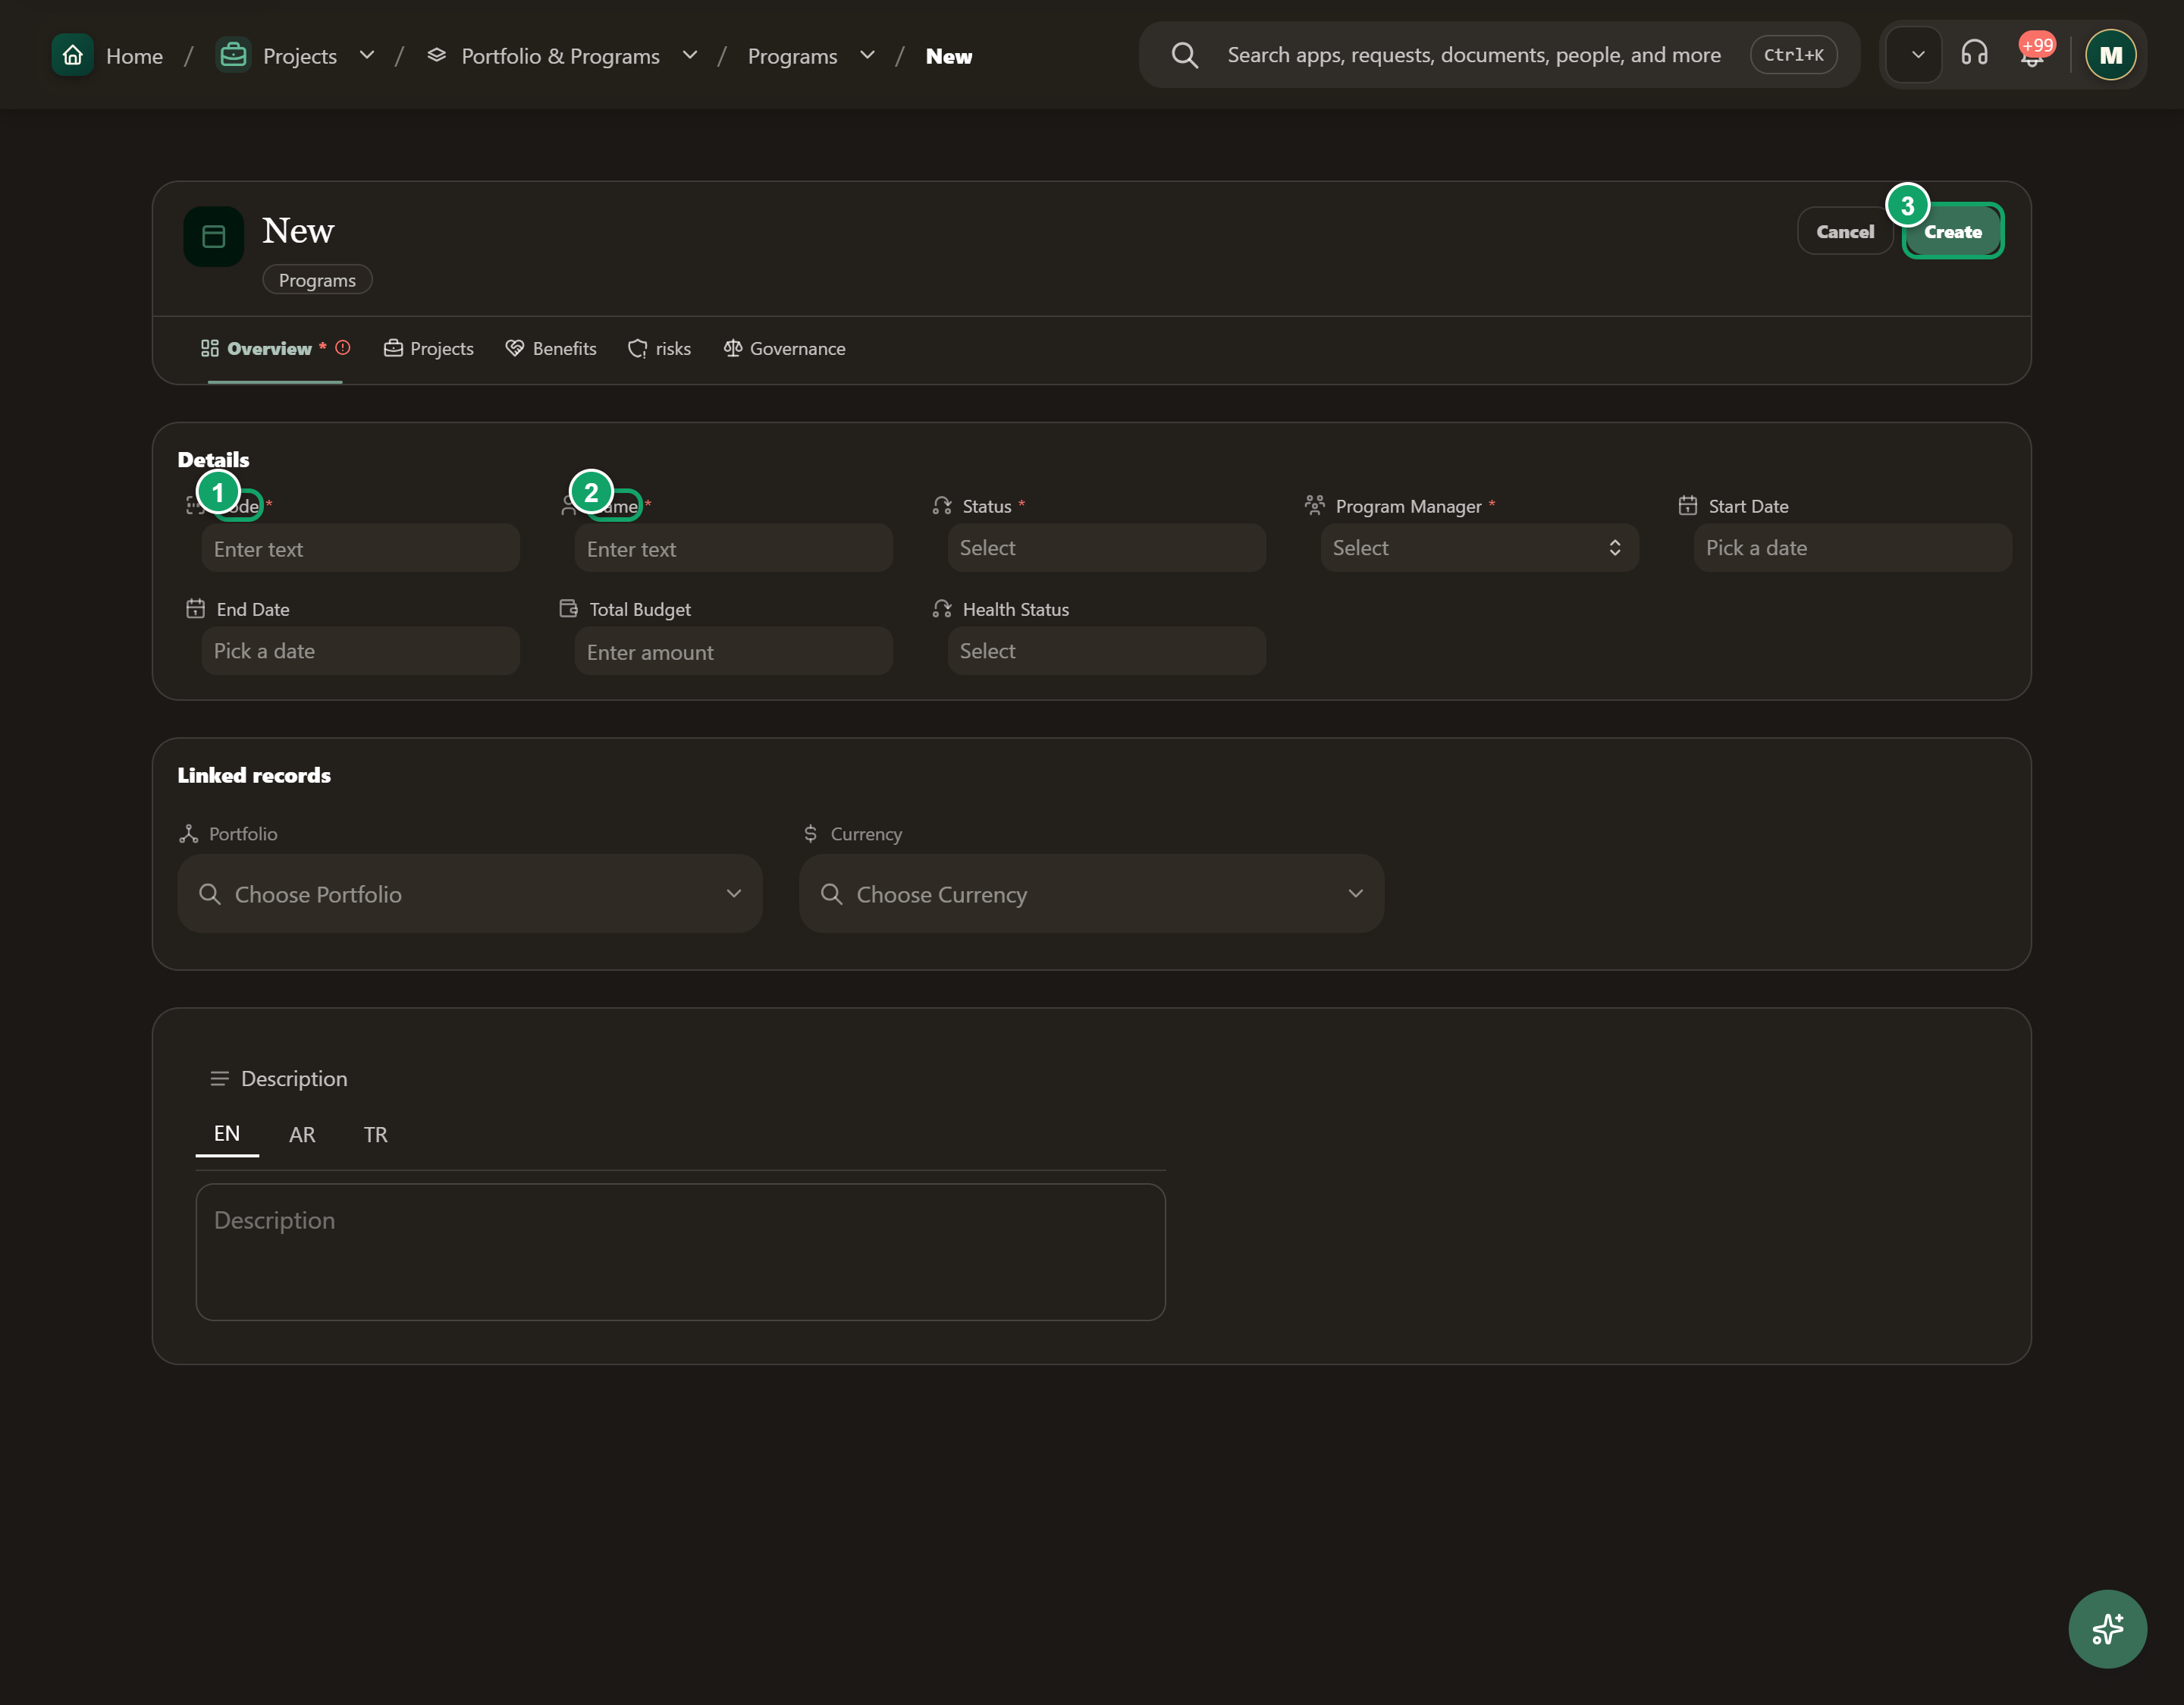
\includegraphics[width=0.95\linewidth,height=0.72\textheight,keepaspectratio]{figures/screens/ch05-programs-en.png}
\caption{A new program before saving}
\label{fig:projects-screen-programs}
\shotnote{The form shows program manager, status, and dates, with an optional portfolio link. These details establish who coordinates related projects; choosing a portfolio does not automatically add projects to the program. ① “Code” and ② “Name”: the first two fields that identify the program. ③ “Create”.}
\end{figure}
\begin{table}[H]
\centering
\caption{What do you record?}
\label{tab:projects-programs-fields}
\begin{tabularx}{\linewidth}{R{4.2cm} Y}
\rcHeaderRow
\thh{Information} & \thh{Fields}\\
Required information & “Code”, “Name”, “Status”, “Program Manager”.\\
Additional information & “Description”, “Portfolio”, “Sponsor”, “Start Date”, “End Date”, “Total Budget”, “Currency”, “Health Status”, “Benefits Summary”, “Strategic Plan”, “Tags”.\\
\end{tabularx}
\end{table}
\begin{table}[H]
\centering
\caption{Tabs and related records}
\label{tab:projects-programs-tabs}
\begin{tabularx}{\linewidth}{R{4.2cm} Y}
\rcHeaderRow
\thh{Tab} & \thh{What it contains}\\
“Overview” & “Program Summary”\\
“Projects” & Projects (\ref{sec:projects-feature-projects})\\
“Benefits” & “Benefit Case”\\
“Financials” & Shows information for this aspect when the record configuration applies.\\
“Delivery” & “Delivery Context”\\
“Governance” & “Governance”; Planning Reviews (\ref{sec:projects-feature-planning-reviews}); Planning Approvals (\ref{sec:projects-feature-planning-approvals}); Planning Decisions (\ref{sec:projects-feature-planning-decisions})\\
\end{tabularx}
\end{table}
\begin{figure}[H]
\centering
\begin{tikzpicture}[node distance=0.5cm]
\node[stepBox] (n0) {Choose work page};
\node[stepBox,below=of n0] (n1) {Programs};
\node[stepBox,below=of n1] (n2) {Save and reopen};
\draw[flowsTo] (n0) -- (n1);
\draw[flowsTo] (n1) -- (n2);
\end{tikzpicture}
\rclegend
\caption{Work and verification path}
\label{fig:projects-programs-flow}
\shotnote{Begin by opening “Programs” and choosing the correct record before entering details. Reopening after saving checks persistence; it does not imply approval or completion of related work.}
\end{figure}

\subsection{Actions and verification}
\begin{enumerate}
\item Open “Programs” and select “Add”. Enter code and name and choose status and program manager.
\item Choose a portfolio if the program belongs to one, then enter expected benefits, dates, and available financial information. Select “Create”.
\item Reopen the program and review its manager and intended benefits. Associate appropriate projects through each project’s program field, then check the related-project list.
\end{enumerate}

\textbf{Try the example:} In the fictional example, use “Branch service improvement” for “Name”, then complete the other information to suit Horizon's work. Example values do not replace the actual records required by relation fields.

\textbf{Check and recover:} The record should be present when reopened, with its saved values. If it is missing, check search, filters, scope, and access before creating another. If saving fails, resolve required fields and validation messages; missing tabs or locked fields require checking record type, framework, and stage with the responsible person.

\clearpage
\section{Budgets}
\label{sec:projects-feature-budgets}

A budget brings cost lines, funding sources, and expenditures into one record. The finance owner reviews planned amounts and recorded actuals before making spending decisions.

\begin{rcnote}[Example: Horizon]
Sarah coordinates with the finance owner to prepare the Aleppo visit budget. The owner records a travel line and compares planned amounts with recorded expenditures for the same currency and period.
\end{rcnote}

\textbf{Where and who:} Open the “Projects” app, then its “Budgets” card. This is a main app page. The person responsible for this work uses it; employees edit only the information their permissions allow.

\begin{figure}[H]
\centering
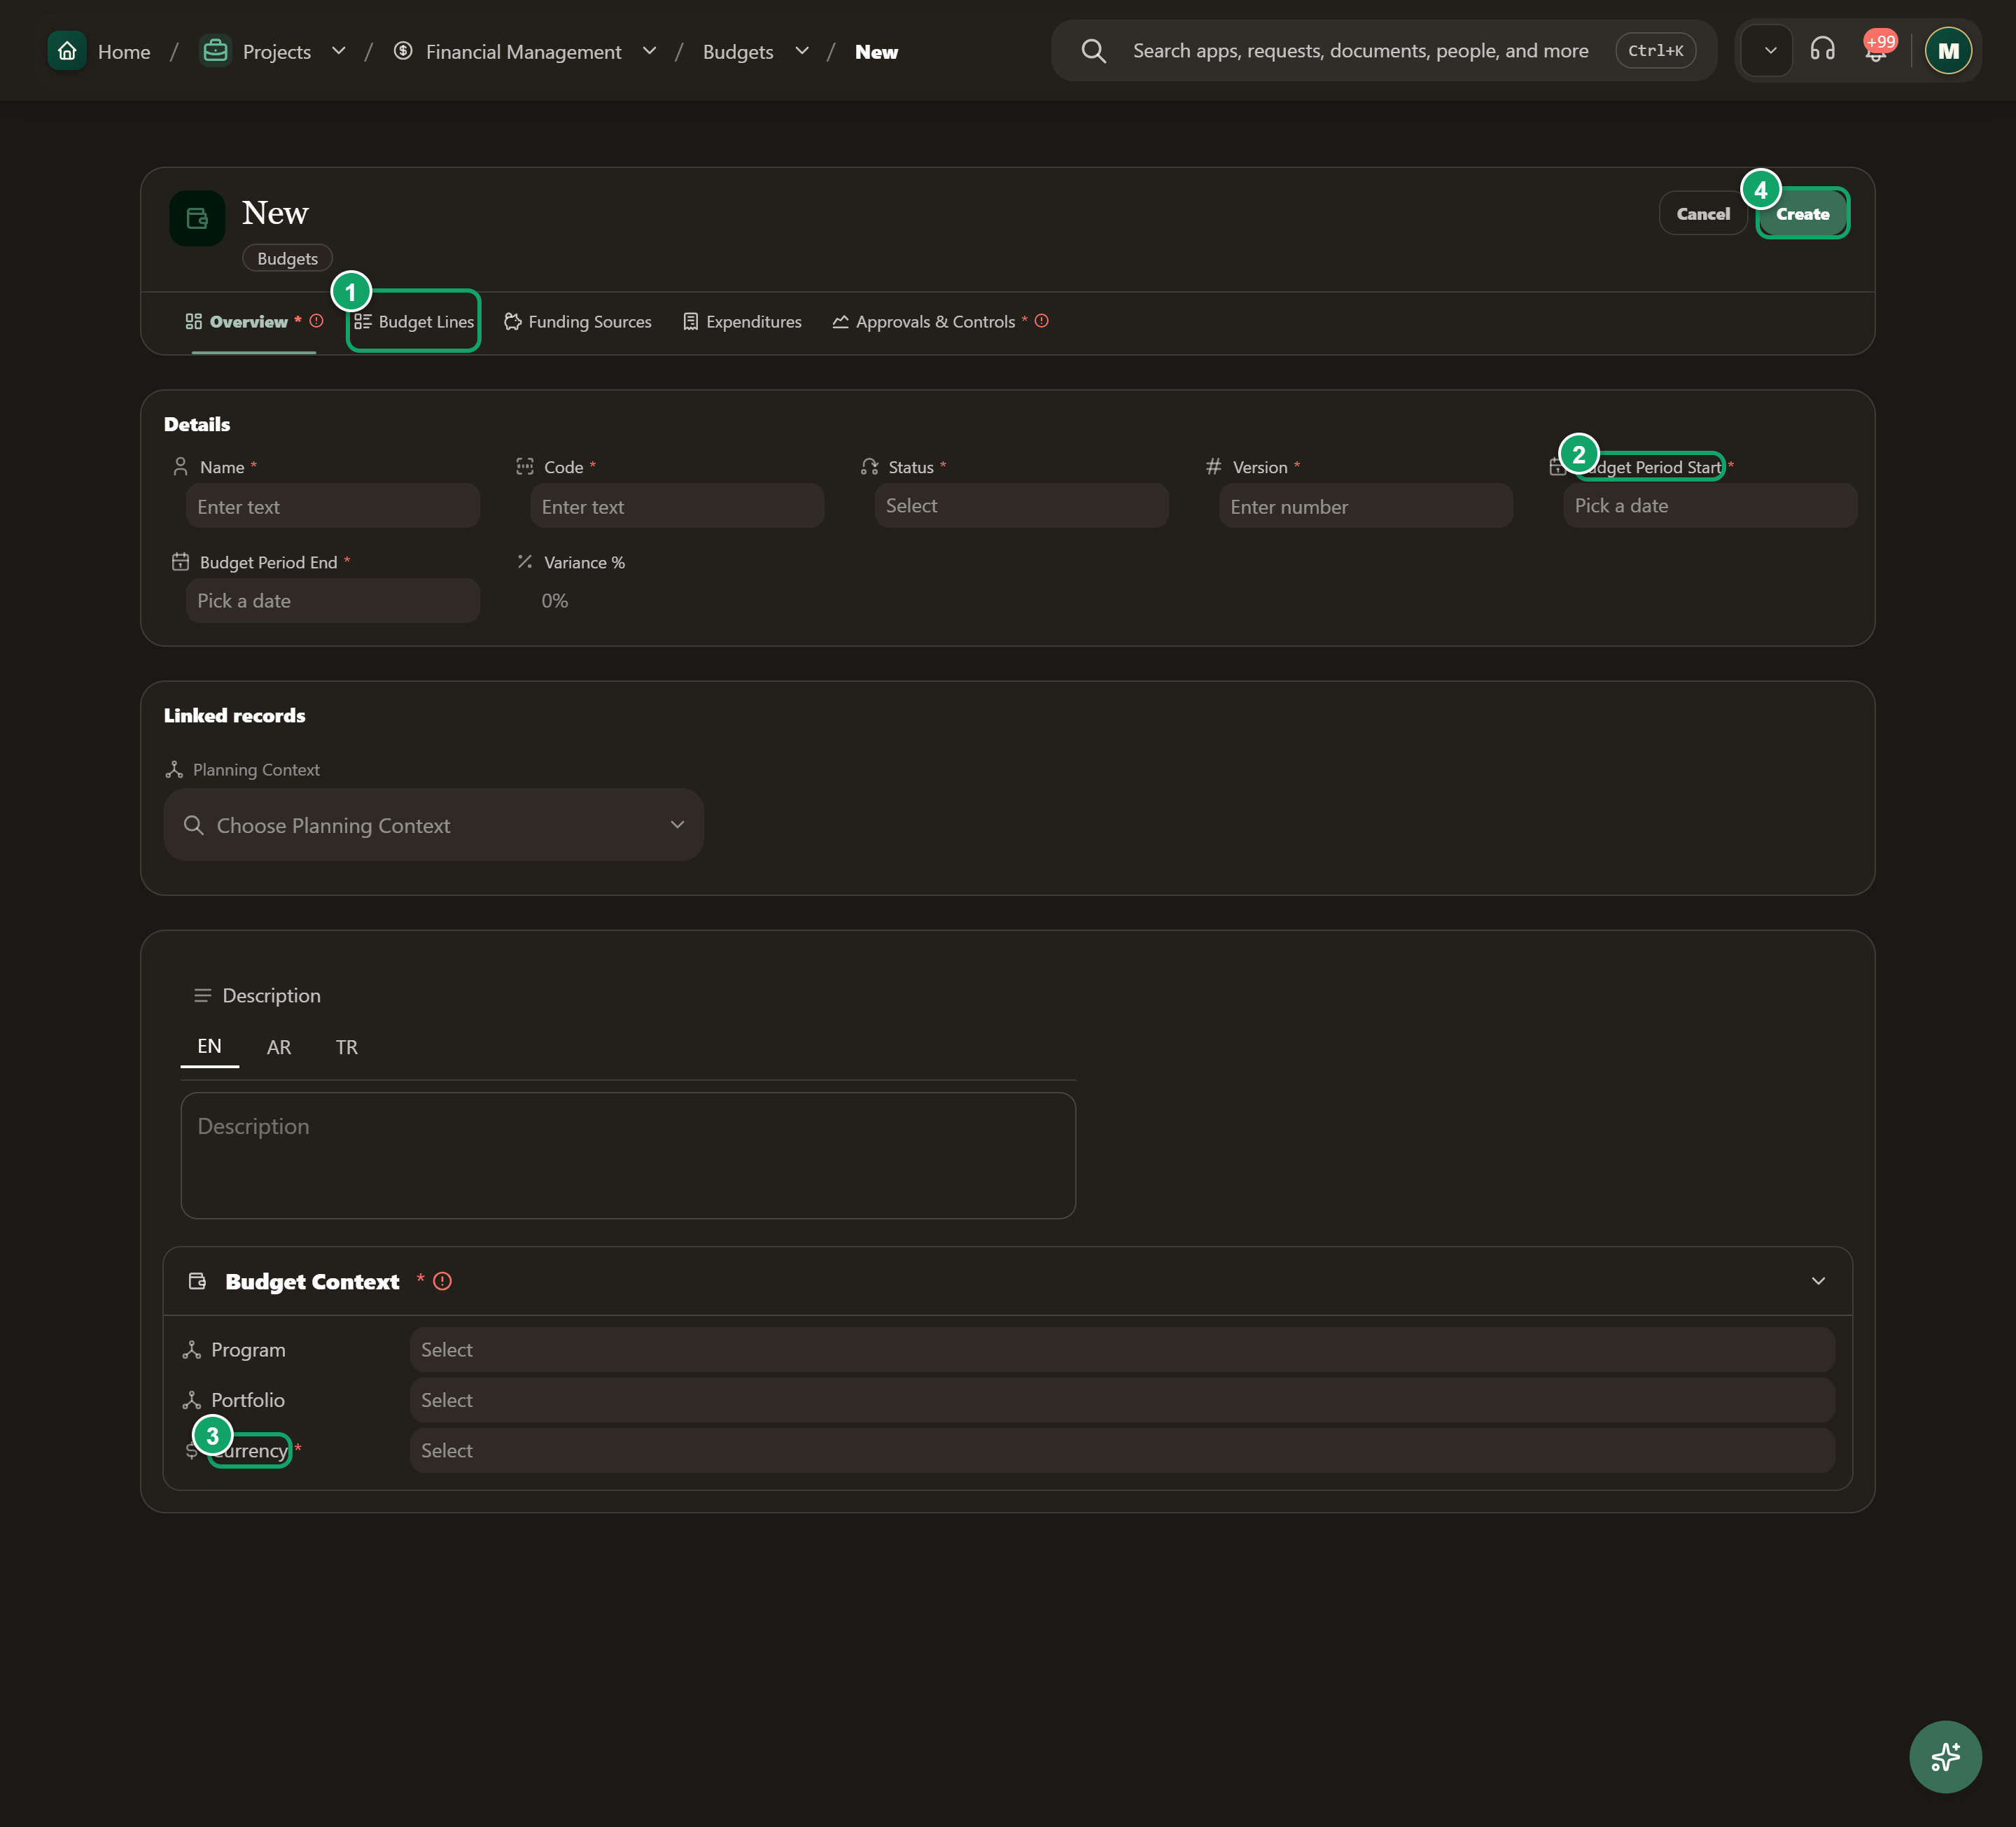
\includegraphics[width=0.95\linewidth,height=0.72\textheight,keepaspectratio]{figures/screens/ch05-budgets-en.png}
\caption{Setting up a new budget before saving}
\label{fig:projects-screen-budgets}
\shotnote{The form ties budget identity and version to a period and currency and allows a work context to be selected. Lines, funding, and expenditures have their own sections, so this screen alone represents neither a complete budget nor a spending transaction. ① The “Budget Lines” tab where amounts are broken down. ② “Budget Period Start”. ③ “Currency” in the budget context. ④ “Create”.}
\end{figure}
\begin{table}[H]
\centering
\caption{What do you record?}
\label{tab:projects-budgets-fields}
\begin{tabularx}{\linewidth}{R{4.2cm} Y}
\rcHeaderRow
\thh{Information} & \thh{Fields}\\
Required information & “Name”, “Code”, “Status”, “Version”, “Current Version”, “Currency”, “Budget Period Start”, “Budget Period End”, “Prepared By”.\\
Additional information & “Description”, “Planning Context”, “Program”, “Portfolio”, “Previous Version”, “Total Planned”, “Total Actual”, “Total Committed”, “Total Available”, “Total Funded”, “Funding Gap”, “Variance \%”, “Contingency Amount”, “Contingency \%”, “Approved By”, “Approval Date”, “Notes”.\\
\end{tabularx}
\end{table}
\begin{table}[H]
\centering
\caption{Tabs and related records}
\label{tab:projects-budgets-tabs}
\begin{tabularx}{\linewidth}{R{4.2cm} Y}
\rcHeaderRow
\thh{Tab} & \thh{What it contains}\\
“Overview” & “Budget Context”; “Budget Totals”\\
“Budget Lines” & Budget Lines (\ref{sec:projects-feature-budget-lines})\\
“Funding Sources” & “Funding Health”; Funding Sources (\ref{sec:projects-feature-funding-sources})\\
“Expenditures” & Expenditures (\ref{sec:projects-feature-expenditures})\\
“Approvals \& Controls” & “Versioning”; “Approvals”; “Forecast Controls”\\
\end{tabularx}
\end{table}
\begin{figure}[H]
\centering
\begin{tikzpicture}[node distance=0.5cm]
\node[stepBox] (n0) {Choose work page};
\node[stepBox,below=of n0] (n1) {Budgets};
\node[stepBox,below=of n1] (n2) {Save and reopen};
\draw[flowsTo] (n0) -- (n1);
\draw[flowsTo] (n1) -- (n2);
\end{tikzpicture}
\rclegend
\caption{Work and verification path}
\label{fig:projects-budgets-flow}
\shotnote{Begin by opening “Budgets” and choosing the correct record before entering details. Reopening after saving checks persistence; it does not imply approval or completion of related work.}
\end{figure}

\subsection{Actions and verification}
\begin{enumerate}
\item Open “Budgets” in Projects and select “Add”. Enter code and name and choose currency and budget period start and end.
\item Review status, version, “Current Version”, and “Prepared By”. Link the budget to the intended work context where appropriate, then select “Create”.
\item Reopen the budget and add its lines through “Budget Lines”. Review each line’s type and costing before interpreting the total.
\item Track funding sources and expenditures in their sections. Check version, currency, and period when comparing figures; distinguish pledged funding, received funding, and paid expenditure.
\end{enumerate}

\textbf{Try the example:} In the fictional example, use “Aleppo visit budget” for “Name”, then complete the other information to suit Horizon's work. Example values do not replace the actual records required by relation fields.

\textbf{Check and recover:} The record should be present when reopened, with its saved values. If it is missing, check search, filters, scope, and access before creating another. If saving fails, resolve required fields and validation messages; missing tabs or locked fields require checking record type, framework, and stage with the responsible person.

\clearpage
\section{Cost Categories}
\label{sec:projects-feature-cost-categories}

Cost categories keep budget lines consistently classified, for example as travel or equipment. The finance owner sets them up so comparable costs do not end up under different names.

\begin{rcnote}[Example: Horizon]
The finance owner creates “Travel and transport” with code \en{HZN-C-01} and type “Travel”. Sarah uses it for the visit team’s travel line, keeping travel costs consistently classified.
\end{rcnote}

\textbf{Where and who:} Open the “Projects” app, then its “Cost Categories” card. This is a main app page. The person responsible for this work uses it; employees edit only the information their permissions allow.

\begin{figure}[H]
\centering
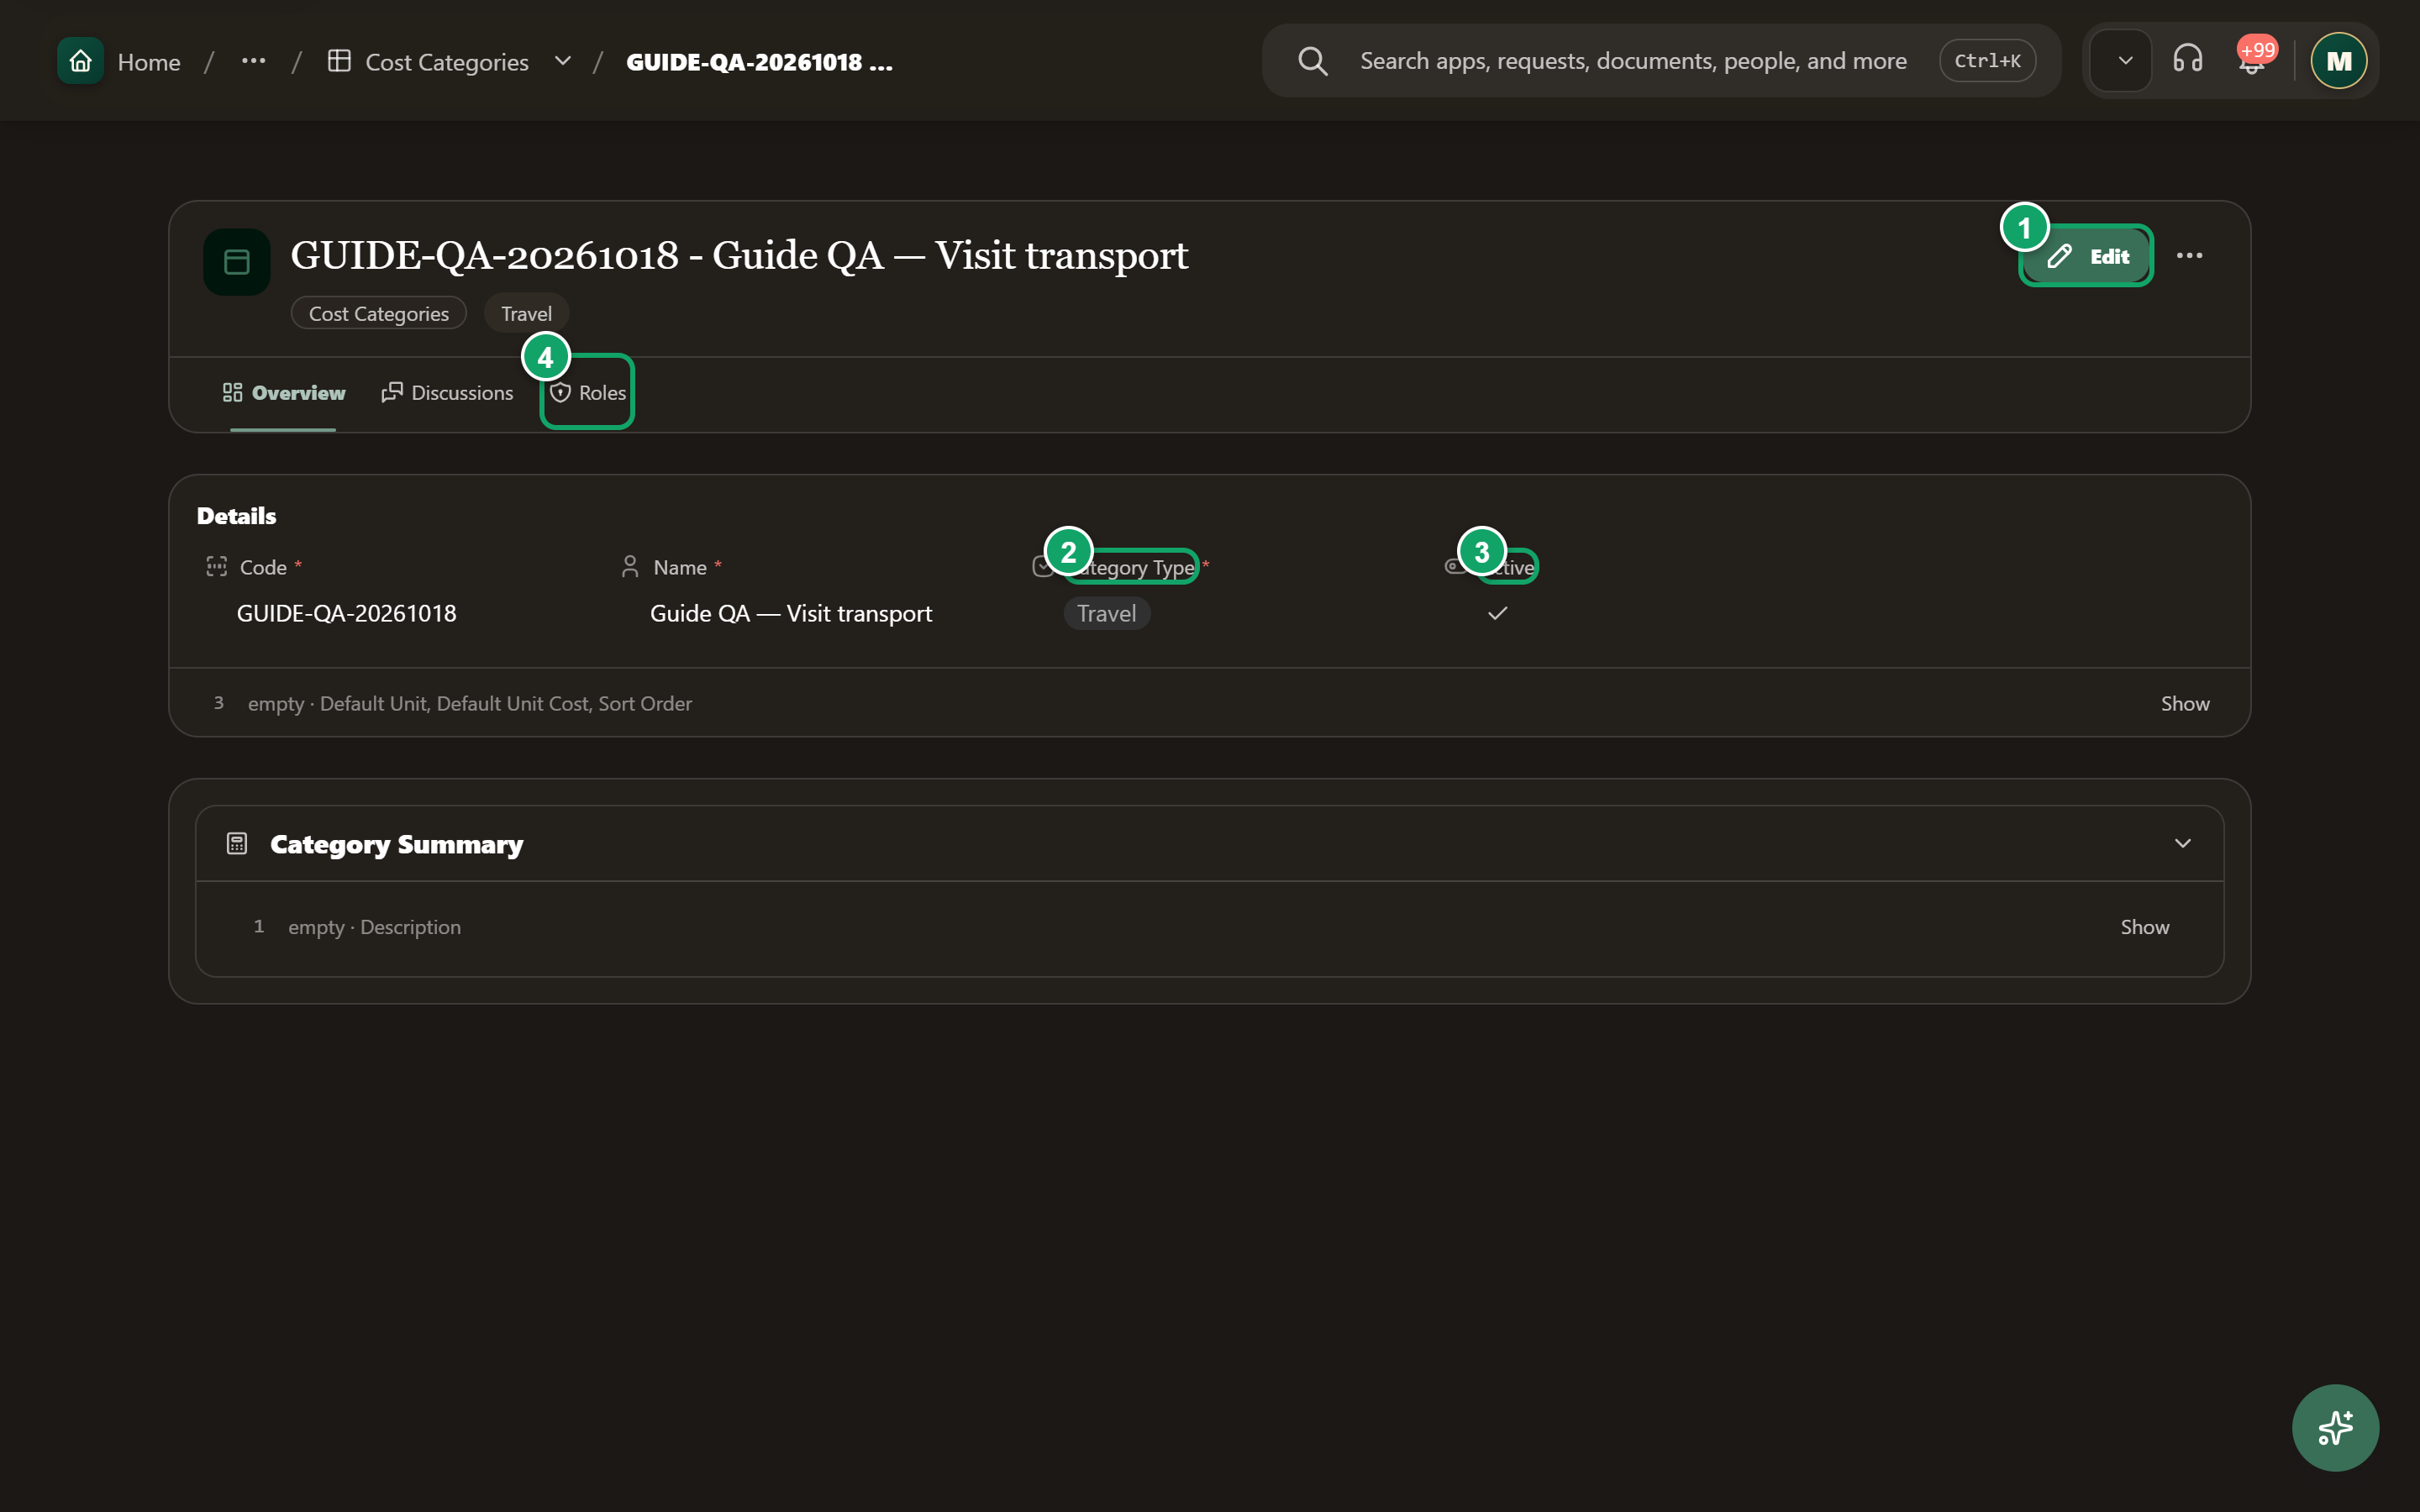
\includegraphics[width=0.95\linewidth,height=0.72\textheight,keepaspectratio]{figures/screens/ch05-cost-category-en.png}
\caption{A test cost category after saving}
\label{fig:projects-screen-cost-category}
\shotnote{The saved record shows its code, name, “Travel” type, and active state. Empty fields can be revealed, so missing unit or cost values do not mean saving failed; this QA record is separate from the fictional Horizon example. ① “Edit”. ② “Category Type”: classifies the cost, here Travel. ③ “Active”: shows the category is available for use. ④ The “Roles” tab for who can see or change the category.}
\end{figure}
\begin{table}[H]
\centering
\caption{What do you record?}
\label{tab:projects-cost-categories-fields}
\begin{tabularx}{\linewidth}{R{4.2cm} Y}
\rcHeaderRow
\thh{Information} & \thh{Fields}\\
Required information & “Code”, “Name”, “Category Type”.\\
Additional information & “Description”, “Active”, “Default Unit”, “Default Unit Cost”, “Sort Order”.\\
\end{tabularx}
\end{table}
\begin{table}[H]
\centering
\caption{Tabs and related records}
\label{tab:projects-cost-categories-tabs}
\begin{tabularx}{\linewidth}{R{4.2cm} Y}
\rcHeaderRow
\thh{Tab} & \thh{What it contains}\\
“Overview” & “Category Summary”\\
\end{tabularx}
\end{table}
\begin{figure}[H]
\centering
\begin{tikzpicture}[node distance=0.5cm]
\node[stepBox] (n0) {Choose work page};
\node[stepBox,below=of n0] (n1) {Cost Categories};
\node[stepBox,below=of n1] (n2) {Save and reopen};
\draw[flowsTo] (n0) -- (n1);
\draw[flowsTo] (n1) -- (n2);
\end{tikzpicture}
\rclegend
\caption{Work and verification path}
\label{fig:projects-cost-categories-flow}
\shotnote{Begin by opening “Cost Categories” and choosing the correct record before entering details. Reopening after saving checks persistence; it does not imply approval or completion of related work.}
\end{figure}

\subsection{Actions and verification}
\begin{enumerate}
\item Open “Cost Categories” and select “Add”. Enter “Code” and “Name”, then choose “Category Type”.
\item Review “Active” and enter a default unit and cost if appropriate. Select “Create” and wait for confirmation.
\item Reopen the category from its list. Check code, name, and type, then use it in the relevant budget line rather than creating another category with the same meaning.
\end{enumerate}

\textbf{Try the example:} In the fictional example, use “Travel and transport” for “Name”, then complete the other information to suit Horizon's work. Example values do not replace the actual records required by relation fields.

\textbf{Check and recover:} The record should be present when reopened, with its saved values. If it is missing, check search, filters, scope, and access before creating another. If saving fails, resolve required fields and validation messages; missing tabs or locked fields require checking record type, framework, and stage with the responsible person.

\clearpage
\section{Planning Themes}
\label{sec:projects-feature-planning-themes}

A strategic theme groups priorities under a clear direction. Use it to organize plan objectives before moving into execution details.

\begin{rcnote}[Example: Horizon]
At Horizon, Sarah reviews “Branch readiness” as part of preparing the Aleppo branch visit. She records the information relevant to that work and checks it appears in the correct record before moving on.
\end{rcnote}

\textbf{Where and who:} Open “Plans” (\ref{sec:projects-feature-plans}), then the relevant record and its “Framework” tab, and then “Planning Themes”. This is a related record within the workspace, not a separate app-menu page. The person responsible for this work uses it; employees edit only the information their permissions allow.

\begin{table}[H]
\centering
\caption{What do you record?}
\label{tab:projects-planning-themes-fields}
\begin{tabularx}{\linewidth}{R{4.2cm} Y}
\rcHeaderRow
\thh{Information} & \thh{Fields}\\
Required information & “Title”.\\
Required when applicable & “Planning Context”. Visibility depends on the record type and configuration.\\
Additional information & “Description”, “Owner”.\\
\end{tabularx}
\end{table}
\begin{figure}[H]
\centering
\begin{tikzpicture}[node distance=0.5cm]
\node[stepBox] (n0) {Planning Themes};
\node[stepBox,below=of n0] (n1) {Planning Context};
\draw[dependsOn] (n0) -- (n1);
\end{tikzpicture}
\rclegend
\caption{The record and its context}
\label{fig:projects-planning-themes-flow}
\shotnote{The “Planning Context” field links this record to an available work context. The field is required when the form applies, so prepare the referenced record before saving. The context can be a plan, project, program, or portfolio as available; you do not need to create all those types.}
\end{figure}

\subsection{Actions and verification}
\begin{enumerate}
\item Open the intended “Plans” record, then “Framework”. Check its name before opening “Planning Themes”.
\item Open the existing record to edit it, or use the list's add action to create a new one. Check the parent link populated by the screen and avoid changing it unintentionally.
\item Complete “Title”. Select links from existing records and review additional fields appearing with your choices.
\item When creating a record, select “Create” and wait for saving to complete. Reopen it from its list and check its values, links, and state.
\end{enumerate}

\textbf{Try the example:} In the fictional example, use “Branch readiness” for “Title”, then complete the other information to suit Horizon's work. Example values do not replace the actual records required by relation fields.

\textbf{Check and recover:} The record should be present when reopened, with its saved values linked to the intended “Plans” record. If it is missing, check search, filters, scope, and access before creating another. If saving fails, resolve required fields and validation messages; missing tabs or locked fields require checking record type, framework, and stage with the responsible person.

\clearpage
\section{Planning Objectives}
\label{sec:projects-feature-planning-objectives}

An objective describes the change a plan should achieve. Link it to the right context, then review its associated indicators rather than relying on a broad title.

\begin{rcnote}[Example: Horizon]
At Horizon, Sarah reviews “Improve visit readiness” as part of preparing the Aleppo branch visit. She records the information relevant to that work and checks it appears in the correct record before moving on.
\end{rcnote}

\textbf{Where and who:} Open “Plans” (\ref{sec:projects-feature-plans}), then the relevant record and its “Framework” tab, and then “Planning Objectives”. This is a related record within the workspace, not a separate app-menu page. The person responsible for this work uses it; employees edit only the information their permissions allow.

\begin{table}[H]
\centering
\caption{What do you record?}
\label{tab:projects-planning-objectives-fields}
\begin{tabularx}{\linewidth}{R{4.2cm} Y}
\rcHeaderRow
\thh{Information} & \thh{Fields}\\
Required information & “Name”, “Status”.\\
Required when applicable & “Planning Context”. Visibility depends on the record type and configuration.\\
Additional information & “Description”, “Objective Type”, “Priority”, “Owner”, “Target Date”.\\
Calculated results & “Progress \%”. Review the source values if a result differs from expectations.\\
\end{tabularx}
\end{table}
\begin{figure}[H]
\centering
\begin{tikzpicture}[node distance=0.5cm]
\node[stepBox] (n0) {Planning Objectives};
\node[stepBox,below=of n0] (n1) {Planning Context};
\draw[dependsOn] (n0) -- (n1);
\end{tikzpicture}
\rclegend
\caption{The record and its context}
\label{fig:projects-planning-objectives-flow}
\shotnote{The “Planning Context” field links this record to an available work context. The field is required when the form applies, so prepare the referenced record before saving. The context can be a plan, project, program, or portfolio as available; you do not need to create all those types.}
\end{figure}

\subsection{Actions and verification}
\begin{enumerate}
\item Open the intended “Plans” record, then “Framework”. Check its name before opening “Planning Objectives”.
\item Open the existing record to edit it, or use the list's add action to create a new one. Check the parent link populated by the screen and avoid changing it unintentionally.
\item Complete “Name”, “Status”. Select links from existing records and review additional fields appearing with your choices.
\item When creating a record, select “Create” and wait for saving to complete. Reopen it from its list and check its values, links, and state.
\end{enumerate}

\textbf{Try the example:} In the fictional example, use “Improve visit readiness” for “Name”, then complete the other information to suit Horizon's work. Example values do not replace the actual records required by relation fields.

\textbf{Check and recover:} The record should be present when reopened, with its saved values linked to the intended “Plans” record. If it is missing, check search, filters, scope, and access before creating another. If saving fails, resolve required fields and validation messages; missing tabs or locked fields require checking record type, framework, and stage with the responsible person.

\clearpage
\section{Planning Initiatives}
\label{sec:projects-feature-planning-initiatives}

An initiative records proposed work that supports strategic direction. Track its ownership and state within the plan; recording it does not automatically create a project.

\begin{rcnote}[Example: Horizon]
At Horizon, Sarah reviews “Standardize visit preparation” as part of preparing the Aleppo branch visit. She records the information relevant to that work and checks it appears in the correct record before moving on.
\end{rcnote}

\textbf{Where and who:} Open “Plans” (\ref{sec:projects-feature-plans}), then the relevant record and its “Initiatives” tab, and then “Planning Initiatives”. This is a related record within the workspace, not a separate app-menu page. The person responsible for this work uses it; employees edit only the information their permissions allow.

\begin{table}[H]
\centering
\caption{What do you record?}
\label{tab:projects-planning-initiatives-fields}
\begin{tabularx}{\linewidth}{R{4.2cm} Y}
\rcHeaderRow
\thh{Information} & \thh{Fields}\\
Required information & “Title”, “Status”.\\
Required when applicable & “Planning Context”. Visibility depends on the record type and configuration.\\
Additional information & “Theme”, “Objective”, “Description”, “Owner”, “Priority”, “Planned Start”, “Planned End”, “Benefit Hypothesis”, “Linked Target”.\\
\end{tabularx}
\end{table}
\begin{figure}[H]
\centering
\begin{tikzpicture}[node distance=0.5cm]
\node[stepBox] (n0) {Planning Initiatives};
\node[stepBox,below=of n0] (n1) {Planning Context};
\draw[dependsOn] (n0) -- (n1);
\end{tikzpicture}
\rclegend
\caption{The record and its context}
\label{fig:projects-planning-initiatives-flow}
\shotnote{The “Planning Context” field links this record to an available work context. The field is required when the form applies, so prepare the referenced record before saving. The context can be a plan, project, program, or portfolio as available; you do not need to create all those types.}
\end{figure}

\subsection{Actions and verification}
\begin{enumerate}
\item Open the intended “Plans” record, then “Initiatives”. Check its name before opening “Planning Initiatives”.
\item Open the existing record to edit it, or use the list's add action to create a new one. Check the parent link populated by the screen and avoid changing it unintentionally.
\item Complete “Title”, “Status”. Select links from existing records and review additional fields appearing with your choices.
\item When creating a record, select “Create” and wait for saving to complete. Reopen it from its list and check its values, links, and state.
\end{enumerate}

\textbf{Try the example:} In the fictional example, use “Standardize visit preparation” for “Title”, then complete the other information to suit Horizon's work. Example values do not replace the actual records required by relation fields.

\textbf{Check and recover:} The record should be present when reopened, with its saved values linked to the intended “Plans” record. If it is missing, check search, filters, scope, and access before creating another. If saving fails, resolve required fields and validation messages; missing tabs or locked fields require checking record type, framework, and stage with the responsible person.

\clearpage
\section{OKR Cycles}
\label{sec:projects-feature-planning-okrs}

An OKR cycle groups a period's objectives and the key results that measure them. Define the cycle first, then add key results and check-ins.

\begin{rcnote}[Example: Horizon]
At Horizon, Sarah reviews “Final-quarter branch readiness” as part of preparing the Aleppo branch visit. She records the information relevant to that work and checks it appears in the correct record before moving on.
\end{rcnote}

\textbf{Where and who:} Open “Plans” (\ref{sec:projects-feature-plans}), then the relevant record and its “Framework” tab, and then “OKR Cycles”. This is a related record within the workspace, not a separate app-menu page. The person responsible for this work uses it; employees edit only the information their permissions allow.

\begin{table}[H]
\centering
\caption{What do you record?}
\label{tab:projects-planning-okrs-fields}
\begin{tabularx}{\linewidth}{R{4.2cm} Y}
\rcHeaderRow
\thh{Information} & \thh{Fields}\\
Required information & “Cycle Name”.\\
Required when applicable & “Planning Context”. Visibility depends on the record type and configuration.\\
Additional information & “Objective”, “Cadence”, “Owner”.\\
\end{tabularx}
\end{table}
\begin{table}[H]
\centering
\caption{Related records}
\label{tab:projects-planning-okrs-children}
\begin{tabularx}{\linewidth}{R{4.2cm} Y}
\rcHeaderRow
\thh{Record} & \thh{Open the explanation}\\
Key Results & \ref{sec:projects-feature-planning-key-results}\\
\end{tabularx}
\end{table}
\begin{figure}[H]
\centering
\begin{tikzpicture}[node distance=0.5cm]
\node[stepBox] (n0) {OKR Cycles};
\node[stepBox,below=of n0] (n1) {Planning Context};
\draw[dependsOn] (n0) -- (n1);
\end{tikzpicture}
\rclegend
\caption{The record and its context}
\label{fig:projects-planning-okrs-flow}
\shotnote{The “Planning Context” field links this record to an available work context. The field is required when the form applies, so prepare the referenced record before saving. The context can be a plan, project, program, or portfolio as available; you do not need to create all those types.}
\end{figure}

\subsection{Actions and verification}
\begin{enumerate}
\item Open the intended “Plans” record, then “Framework”. Check its name before opening “OKR Cycles”.
\item Open the existing record to edit it, or use the list's add action to create a new one. Check the parent link populated by the screen and avoid changing it unintentionally.
\item Complete “Cycle Name”. Select links from existing records and review additional fields appearing with your choices.
\item When creating a record, select “Create” and wait for saving to complete. Reopen it from its list and check its values, links, and state.
\end{enumerate}

\textbf{Try the example:} In the fictional example, use “Final-quarter branch readiness” for “Cycle Name”, then complete the other information to suit Horizon's work. Example values do not replace the actual records required by relation fields.

\textbf{Check and recover:} The record should be present when reopened, with its saved values linked to the intended “Plans” record. If it is missing, check search, filters, scope, and access before creating another. If saving fails, resolve required fields and validation messages; missing tabs or locked fields require checking record type, framework, and stage with the responsible person.

\clearpage
\section{Key Results}
\label{sec:projects-feature-planning-key-results}

A key result turns an objective into something trackable. Choose the appropriate tracking mode and distinguish the target from the actual result.

\begin{rcnote}[Example: Horizon]
At Horizon, Sarah reviews “Visit preparation complete” as part of preparing the Aleppo branch visit. She records the information relevant to that work and checks it appears in the correct record before moving on.
\end{rcnote}

\textbf{Where and who:} Open “Plans” (\ref{sec:projects-feature-plans}), then the relevant record and its “Framework” tab, and then “Key Results”. This is a related record within the workspace, not a separate app-menu page. The person responsible for this work uses it; employees edit only the information their permissions allow.

\begin{table}[H]
\centering
\caption{What do you record?}
\label{tab:projects-planning-key-results-fields}
\begin{tabularx}{\linewidth}{R{4.2cm} Y}
\rcHeaderRow
\thh{Information} & \thh{Fields}\\
Required information & “OKR Cycle”, “Tracking Mode”, “Name”, “Commitment Type”.\\
Required when applicable & “Planning Context”. Visibility depends on the record type and configuration.\\
Additional information & “Indicator”, “Scoring Method”, “Target Value”, “Start Value”, “Target Value (Number)”, “Confidence”, “Cadence State”, “Status”.\\
Calculated results & “Current Value”, “Current Value (Number)”, “Score \%”, “Last Check-in”. Review the source values if a result differs from expectations.\\
\end{tabularx}
\end{table}
\begin{figure}[H]
\centering
\begin{tikzpicture}[node distance=0.5cm]
\node[stepBox] (n0) {Key Results};
\node[stepBox,below=of n0] (n1) {Planning Context};
\draw[dependsOn] (n0) -- (n1);
\end{tikzpicture}
\rclegend
\caption{The record and its context}
\label{fig:projects-planning-key-results-flow}
\shotnote{The “Planning Context” field links this record to an available work context. The field is required when the form applies, so prepare the referenced record before saving. The context can be a plan, project, program, or portfolio as available; you do not need to create all those types.}
\end{figure}

\subsection{Actions and verification}
\begin{enumerate}
\item Open the intended “Plans” record, then “Framework”. Check its name before opening “Key Results”.
\item Open the existing record to edit it, or use the list's add action to create a new one. Check the parent link populated by the screen and avoid changing it unintentionally.
\item Complete “OKR Cycle”, “Tracking Mode”, “Name”, “Commitment Type”. Select links from existing records and review additional fields appearing with your choices.
\item When creating a record, select “Create” and wait for saving to complete. Reopen it from its list and check its values, links, and state.
\end{enumerate}

\textbf{Try the example:} In the fictional example, use “Visit preparation complete” for “Name”, then complete the other information to suit Horizon's work. Example values do not replace the actual records required by relation fields.

\textbf{Check and recover:} The record should be present when reopened, with its saved values linked to the intended “Plans” record. If it is missing, check search, filters, scope, and access before creating another. If saving fails, resolve required fields and validation messages; missing tabs or locked fields require checking record type, framework, and stage with the responsible person.

\clearpage
\section{Key Result Check-ins}
\label{sec:projects-feature-planning-key-result-checkins}

A key-result check-in records its state on a particular date. Successive updates help explain progress and obstacles instead of relying on the latest number alone.

\begin{rcnote}[Example: Horizon]
At Horizon, Sarah reviews “Visit checklist readiness check” as part of preparing the Aleppo branch visit. She records the information relevant to that work and checks it appears in the correct record before moving on.
\end{rcnote}

\textbf{Where and who:} Open “Plans” (\ref{sec:projects-feature-plans}), then the relevant record and its “Framework” tab, and then “Key Result Check-ins”. This is a related record within the workspace, not a separate app-menu page. The person responsible for this work uses it; employees edit only the information their permissions allow.

\begin{table}[H]
\centering
\caption{What do you record?}
\label{tab:projects-planning-key-result-checkins-fields}
\begin{tabularx}{\linewidth}{R{4.2cm} Y}
\rcHeaderRow
\thh{Information} & \thh{Fields}\\
Required information & “Key Result”, “Check-in Date”, “Status”.\\
Required when applicable & “Planning Context”. Visibility depends on the record type and configuration.\\
Additional information & “Value (Number)”, “Value (Text)”, “Score \%”, “Confidence”, “Summary”.\\
\end{tabularx}
\end{table}
\begin{figure}[H]
\centering
\begin{tikzpicture}[node distance=0.5cm]
\node[stepBox] (n0) {Key Result Check-ins};
\node[stepBox,below=of n0] (n1) {Planning Context};
\draw[dependsOn] (n0) -- (n1);
\end{tikzpicture}
\rclegend
\caption{The record and its context}
\label{fig:projects-planning-key-result-checkins-flow}
\shotnote{The “Planning Context” field links this record to an available work context. The field is required when the form applies, so prepare the referenced record before saving. The context can be a plan, project, program, or portfolio as available; you do not need to create all those types.}
\end{figure}

\subsection{Actions and verification}
\begin{enumerate}
\item Open the intended “Plans” record, then “Framework”. Check its name before opening “Key Result Check-ins”.
\item Open the existing record to edit it, or use the list's add action to create a new one. Check the parent link populated by the screen and avoid changing it unintentionally.
\item Complete “Key Result”, “Check-in Date”, “Status”. Select links from existing records and review additional fields appearing with your choices.
\item When creating a record, select “Create” and wait for saving to complete. Reopen it from its list and check its values, links, and state.
\end{enumerate}

\textbf{Check and recover:} The record should be present when reopened, with its saved values linked to the intended “Plans” record. If it is missing, check search, filters, scope, and access before creating another. If saving fails, resolve required fields and validation messages; missing tabs or locked fields require checking record type, framework, and stage with the responsible person.

\clearpage
\section{Hoshin Items}
\label{sec:projects-feature-planning-hoshin-items}

Hoshin connects longer-term direction with annual objectives and the work needed. Identify each item's type so strategic results remain distinct from execution actions.

\begin{rcnote}[Example: Horizon]
At Horizon, Sarah reviews “Improve visit consistency” as part of preparing the Aleppo branch visit. She records the information relevant to that work and checks it appears in the correct record before moving on.
\end{rcnote}

\textbf{Where and who:} Open “Plans” (\ref{sec:projects-feature-plans}), then the relevant record and its “Framework” tab, and then “Hoshin Items”. This is a related record within the workspace, not a separate app-menu page. The person responsible for this work uses it; employees edit only the information their permissions allow.

\begin{table}[H]
\centering
\caption{What do you record?}
\label{tab:projects-planning-hoshin-items-fields}
\begin{tabularx}{\linewidth}{R{4.2cm} Y}
\rcHeaderRow
\thh{Information} & \thh{Fields}\\
Required information & “Item Name”, “Item Type”.\\
Required when applicable & “Planning Context”. Visibility depends on the record type and configuration.\\
Additional information & “Objective”, “Owner”, “X-Matrix Axis”, “Due Date”, “Status”.\\
\end{tabularx}
\end{table}
\begin{figure}[H]
\centering
\begin{tikzpicture}[node distance=0.5cm]
\node[stepBox] (n0) {Hoshin Items};
\node[stepBox,below=of n0] (n1) {Planning Context};
\draw[dependsOn] (n0) -- (n1);
\end{tikzpicture}
\rclegend
\caption{The record and its context}
\label{fig:projects-planning-hoshin-items-flow}
\shotnote{The “Planning Context” field links this record to an available work context. The field is required when the form applies, so prepare the referenced record before saving. The context can be a plan, project, program, or portfolio as available; you do not need to create all those types.}
\end{figure}

\subsection{Actions and verification}
\begin{enumerate}
\item Open the intended “Plans” record, then “Framework”. Check its name before opening “Hoshin Items”.
\item Open the existing record to edit it, or use the list's add action to create a new one. Check the parent link populated by the screen and avoid changing it unintentionally.
\item Complete “Item Name”, “Item Type”. Select links from existing records and review additional fields appearing with your choices.
\item When creating a record, select “Create” and wait for saving to complete. Reopen it from its list and check its values, links, and state.
\end{enumerate}

\textbf{Try the example:} In the fictional example, use “Improve visit consistency” for “Item Name”, then complete the other information to suit Horizon's work. Example values do not replace the actual records required by relation fields.

\textbf{Check and recover:} The record should be present when reopened, with its saved values linked to the intended “Plans” record. If it is missing, check search, filters, scope, and access before creating another. If saving fails, resolve required fields and validation messages; missing tabs or locked fields require checking record type, framework, and stage with the responsible person.

\clearpage
\section{Hoshin X-Matrix Links}
\label{sec:projects-feature-planning-hoshin-x-matrix-links}

Hoshin matrix links show how one item supports another. Choose the source, target, and link type, then check that the relationship conveys the intended meaning.

\begin{rcnote}[Example: Horizon]
At Horizon, Sarah reviews “Connect branch readiness to visits” as part of preparing the Aleppo branch visit. She records the information relevant to that work and checks it appears in the correct record before moving on.
\end{rcnote}

\textbf{Where and who:} Open “Plans” (\ref{sec:projects-feature-plans}), then the relevant record and its “Framework” tab, and then “Hoshin X-Matrix Links”. This is a related record within the workspace, not a separate app-menu page. The person responsible for this work uses it; employees edit only the information their permissions allow.

\begin{table}[H]
\centering
\caption{What do you record?}
\label{tab:projects-planning-hoshin-x-matrix-links-fields}
\begin{tabularx}{\linewidth}{R{4.2cm} Y}
\rcHeaderRow
\thh{Information} & \thh{Fields}\\
Required information & “Source Item”, “Target Item”, “Link Type”.\\
Required when applicable & “Planning Context”. Visibility depends on the record type and configuration.\\
Additional information & “Strength”, “Notes”.\\
\end{tabularx}
\end{table}
\begin{figure}[H]
\centering
\begin{tikzpicture}[node distance=0.5cm]
\node[stepBox] (n0) {Hoshin X-Matrix Links};
\node[stepBox,below=of n0] (n1) {Planning Context};
\draw[dependsOn] (n0) -- (n1);
\end{tikzpicture}
\rclegend
\caption{The record and its context}
\label{fig:projects-planning-hoshin-x-matrix-links-flow}
\shotnote{The “Planning Context” field links this record to an available work context. The field is required when the form applies, so prepare the referenced record before saving. The context can be a plan, project, program, or portfolio as available; you do not need to create all those types.}
\end{figure}

\subsection{Actions and verification}
\begin{enumerate}
\item Open the intended “Plans” record, then “Framework”. Check its name before opening “Hoshin X-Matrix Links”.
\item Open the existing record to edit it, or use the list's add action to create a new one. Check the parent link populated by the screen and avoid changing it unintentionally.
\item Complete “Source Item”, “Target Item”, “Link Type”. Select links from existing records and review additional fields appearing with your choices.
\item When creating a record, select “Create” and wait for saving to complete. Reopen it from its list and check its values, links, and state.
\end{enumerate}

\textbf{Check and recover:} The record should be present when reopened, with its saved values linked to the intended “Plans” record. If it is missing, check search, filters, scope, and access before creating another. If saving fails, resolve required fields and validation messages; missing tabs or locked fields require checking record type, framework, and stage with the responsible person.

\clearpage
\section{Hoshin Catchball Exchanges}
\label{sec:projects-feature-planning-hoshin-catchball-exchanges}

Catchball exchanges record proposals and responses about a Hoshin item. Keep the exchange date and response state so agreements remain distinct from open discussion.

\begin{rcnote}[Example: Horizon]
At Horizon, Sarah reviews “Review Aleppo branch capacity” as part of preparing the Aleppo branch visit. She records the information relevant to that work and checks it appears in the correct record before moving on.
\end{rcnote}

\textbf{Where and who:} Open “Plans” (\ref{sec:projects-feature-plans}), then the relevant record and its “Framework” tab, and then “Hoshin Catchball Exchanges”. This is a related record within the workspace, not a separate app-menu page. The person responsible for this work uses it; employees edit only the information their permissions allow.

\begin{table}[H]
\centering
\caption{What do you record?}
\label{tab:projects-planning-hoshin-catchball-exchanges-fields}
\begin{tabularx}{\linewidth}{R{4.2cm} Y}
\rcHeaderRow
\thh{Information} & \thh{Fields}\\
Required information & “Hoshin Item”, “Exchange Date”, “Response State”.\\
Required when applicable & “Planning Context”. Visibility depends on the record type and configuration.\\
Additional information & “Sender”, “Receiver”, “Summary”, “Decision”.\\
\end{tabularx}
\end{table}
\begin{figure}[H]
\centering
\begin{tikzpicture}[node distance=0.5cm]
\node[stepBox] (n0) {Hoshin Catchball\\Exchanges};
\node[stepBox,below=of n0] (n1) {Planning Context};
\draw[dependsOn] (n0) -- (n1);
\end{tikzpicture}
\rclegend
\caption{The record and its context}
\label{fig:projects-planning-hoshin-catchball-exchanges-flow}
\shotnote{The “Planning Context” field links this record to an available work context. The field is required when the form applies, so prepare the referenced record before saving. The context can be a plan, project, program, or portfolio as available; you do not need to create all those types.}
\end{figure}

\subsection{Actions and verification}
\begin{enumerate}
\item Open the intended “Plans” record, then “Framework”. Check its name before opening “Hoshin Catchball Exchanges”.
\item Open the existing record to edit it, or use the list's add action to create a new one. Check the parent link populated by the screen and avoid changing it unintentionally.
\item Complete “Hoshin Item”, “Exchange Date”, “Response State”. Select links from existing records and review additional fields appearing with your choices.
\item When creating a record, select “Create” and wait for saving to complete. Reopen it from its list and check its values, links, and state.
\end{enumerate}

\textbf{Check and recover:} The record should be present when reopened, with its saved values linked to the intended “Plans” record. If it is missing, check search, filters, scope, and access before creating another. If saving fails, resolve required fields and validation messages; missing tabs or locked fields require checking record type, framework, and stage with the responsible person.

\clearpage
\section{Hoshin Countermeasures}
\label{sec:projects-feature-planning-hoshin-countermeasures}

A countermeasure records a response to a struggling Hoshin item. Link it to the affected item, describe the action, and track its state.

\begin{rcnote}[Example: Horizon]
At Horizon, Sarah reviews “Complete missing visit checklist data” as part of preparing the Aleppo branch visit. She records the information relevant to that work and checks it appears in the correct record before moving on.
\end{rcnote}

\textbf{Where and who:} Open “Plans” (\ref{sec:projects-feature-plans}), then the relevant record and its “Framework” tab, and then “Hoshin Countermeasures”. This is a related record within the workspace, not a separate app-menu page. The person responsible for this work uses it; employees edit only the information their permissions allow.

\begin{table}[H]
\centering
\caption{What do you record?}
\label{tab:projects-planning-hoshin-countermeasures-fields}
\begin{tabularx}{\linewidth}{R{4.2cm} Y}
\rcHeaderRow
\thh{Information} & \thh{Fields}\\
Required information & “Hoshin Item”, “Title”, “Status”.\\
Required when applicable & “Planning Context”. Visibility depends on the record type and configuration.\\
Additional information & “Owner”, “Due Date”, “Progress \%”.\\
\end{tabularx}
\end{table}
\begin{figure}[H]
\centering
\begin{tikzpicture}[node distance=0.5cm]
\node[stepBox] (n0) {Hoshin Countermeasures};
\node[stepBox,below=of n0] (n1) {Planning Context};
\draw[dependsOn] (n0) -- (n1);
\end{tikzpicture}
\rclegend
\caption{The record and its context}
\label{fig:projects-planning-hoshin-countermeasures-flow}
\shotnote{The “Planning Context” field links this record to an available work context. The field is required when the form applies, so prepare the referenced record before saving. The context can be a plan, project, program, or portfolio as available; you do not need to create all those types.}
\end{figure}

\subsection{Actions and verification}
\begin{enumerate}
\item Open the intended “Plans” record, then “Framework”. Check its name before opening “Hoshin Countermeasures”.
\item Open the existing record to edit it, or use the list's add action to create a new one. Check the parent link populated by the screen and avoid changing it unintentionally.
\item Complete “Hoshin Item”, “Title”, “Status”. Select links from existing records and review additional fields appearing with your choices.
\item When creating a record, select “Create” and wait for saving to complete. Reopen it from its list and check its values, links, and state.
\end{enumerate}

\textbf{Try the example:} In the fictional example, use “Complete missing visit checklist data” for “Title”, then complete the other information to suit Horizon's work. Example values do not replace the actual records required by relation fields.

\textbf{Check and recover:} The record should be present when reopened, with its saved values linked to the intended “Plans” record. If it is missing, check search, filters, scope, and access before creating another. If saving fails, resolve required fields and validation messages; missing tabs or locked fields require checking record type, framework, and stage with the responsible person.

\clearpage
\section{Planning Assumptions}
\label{sec:projects-feature-planning-assumptions}

Assumptions record conditions the plan relies on but has not yet confirmed. Review their state as circumstances change; an invalid assumption may require replanning.

\begin{rcnote}[Example: Horizon]
At Horizon, Sarah reviews “Branch team available on visit day” as part of preparing the Aleppo branch visit. She records the information relevant to that work and checks it appears in the correct record before moving on.
\end{rcnote}

\textbf{Where and who:} Open “Plans” (\ref{sec:projects-feature-plans}), then the relevant record and its “Assumptions” tab, and then “Planning Assumptions”. This is a related record within the workspace, not a separate app-menu page. The person responsible for this work uses it; employees edit only the information their permissions allow.

\begin{table}[H]
\centering
\caption{What do you record?}
\label{tab:projects-planning-assumptions-fields}
\begin{tabularx}{\linewidth}{R{4.2cm} Y}
\rcHeaderRow
\thh{Information} & \thh{Fields}\\
Required information & “Assumption”, “Status”.\\
Required when applicable & “Planning Context”. Visibility depends on the record type and configuration.\\
Additional information & “Linked Component”, “Valid Until”.\\
\end{tabularx}
\end{table}
\begin{figure}[H]
\centering
\begin{tikzpicture}[node distance=0.5cm]
\node[stepBox] (n0) {Planning Assumptions};
\node[stepBox,below=of n0] (n1) {Planning Context};
\draw[dependsOn] (n0) -- (n1);
\end{tikzpicture}
\rclegend
\caption{The record and its context}
\label{fig:projects-planning-assumptions-flow}
\shotnote{The “Planning Context” field links this record to an available work context. The field is required when the form applies, so prepare the referenced record before saving. The context can be a plan, project, program, or portfolio as available; you do not need to create all those types.}
\end{figure}

\subsection{Actions and verification}
\begin{enumerate}
\item Open the intended “Plans” record, then “Assumptions”. Check its name before opening “Planning Assumptions”.
\item Open the existing record to edit it, or use the list's add action to create a new one. Check the parent link populated by the screen and avoid changing it unintentionally.
\item Complete “Assumption”, “Status”. Select links from existing records and review additional fields appearing with your choices.
\item When creating a record, select “Create” and wait for saving to complete. Reopen it from its list and check its values, links, and state.
\end{enumerate}

\textbf{Try the example:} In the fictional example, use “Branch team available on visit day” for “Assumption”, then complete the other information to suit Horizon's work. Example values do not replace the actual records required by relation fields.

\textbf{Check and recover:} The record should be present when reopened, with its saved values linked to the intended “Plans” record. If it is missing, check search, filters, scope, and access before creating another. If saving fails, resolve required fields and validation messages; missing tabs or locked fields require checking record type, framework, and stage with the responsible person.

\clearpage
\section{Planning Milestones}
\label{sec:projects-feature-planning-milestones}

A milestone marks a significant result that can be checked. Assign its owner and due date, then review its state when the date arrives.

\begin{rcnote}[Example: Horizon]
At Horizon, Sarah reviews “Visit checklist approved” as part of preparing the Aleppo branch visit. She records the information relevant to that work and checks it appears in the correct record before moving on.
\end{rcnote}

\textbf{Where and who:} Open “Plans” (\ref{sec:projects-feature-plans}), then the relevant record and its “Execution” tab, and then “Planning Milestones”. This is a related record within the workspace, not a separate app-menu page. The person responsible for this work uses it; employees edit only the information their permissions allow.

\begin{table}[H]
\centering
\caption{What do you record?}
\label{tab:projects-planning-milestones-fields}
\begin{tabularx}{\linewidth}{R{4.2cm} Y}
\rcHeaderRow
\thh{Information} & \thh{Fields}\\
Required information & “Name”, “Owner”, “Due Date”, “Status”.\\
Required when applicable & “Planning Context”. Visibility depends on the record type and configuration.\\
Additional information & “Linked Component”, “Description”, “Baseline Date”, “Forecast Date”, “Actual Date”, “Gate Type”, “Critical Milestone”, “Gate Decision”, “Variance Reason”.\\
\end{tabularx}
\end{table}
\begin{figure}[H]
\centering
\begin{tikzpicture}[node distance=0.5cm]
\node[stepBox] (n0) {Planning Milestones};
\node[stepBox,below=of n0] (n1) {Planning Context};
\draw[dependsOn] (n0) -- (n1);
\end{tikzpicture}
\rclegend
\caption{The record and its context}
\label{fig:projects-planning-milestones-flow}
\shotnote{The “Planning Context” field links this record to an available work context. The field is required when the form applies, so prepare the referenced record before saving. The context can be a plan, project, program, or portfolio as available; you do not need to create all those types.}
\end{figure}

\subsection{Actions and verification}
\begin{enumerate}
\item Open the intended “Plans” record, then “Execution”. Check its name before opening “Planning Milestones”.
\item Open the existing record to edit it, or use the list's add action to create a new one. Check the parent link populated by the screen and avoid changing it unintentionally.
\item Complete “Name”, “Owner”, “Due Date”, “Status”. Select links from existing records and review additional fields appearing with your choices.
\item When creating a record, select “Create” and wait for saving to complete. Reopen it from its list and check its values, links, and state.
\end{enumerate}

\textbf{Try the example:} In the fictional example, use “Visit checklist approved” for “Name”, then complete the other information to suit Horizon's work. Example values do not replace the actual records required by relation fields.

\textbf{Check and recover:} The record should be present when reopened, with its saved values linked to the intended “Plans” record. If it is missing, check search, filters, scope, and access before creating another. If saving fails, resolve required fields and validation messages; missing tabs or locked fields require checking record type, framework, and stage with the responsible person.

\clearpage
\section{Project Phases}
\label{sec:projects-feature-phases}

A phase divides the project into ordered periods whose completion can be reviewed. Set its order and dates, and review gate controls when the project uses stage gates.

\begin{rcnote}[Example: Horizon]
At Horizon, Sarah reviews “Visit preparation” as part of preparing the Aleppo branch visit. She records the information relevant to that work and checks it appears in the correct record before moving on.
\end{rcnote}

\textbf{Where and who:} Open “Projects” (\ref{sec:projects-feature-projects}), then the relevant record and its “Schedule” tab, and then “Project Phases”. This is a related record within the workspace, not a separate app-menu page. The person responsible for this work uses it; employees edit only the information their permissions allow.

\begin{table}[H]
\centering
\caption{What do you record?}
\label{tab:projects-phases-fields}
\begin{tabularx}{\linewidth}{R{4.2cm} Y}
\rcHeaderRow
\thh{Information} & \thh{Fields}\\
Required information & “Name”, “Order”, “Status”.\\
Required when applicable & “Project”. Visibility depends on the record type and configuration.\\
Additional information & “Description”, “Phase Type”, “Planned Start Date”, “Planned End Date”, “Actual Start Date”, “Actual End Date”, “Gate Review Required”, “Gate Review”, “Exit Criteria”, “Notes”.\\
\end{tabularx}
\end{table}
\begin{table}[H]
\centering
\caption{Tabs and related records}
\label{tab:projects-phases-tabs}
\begin{tabularx}{\linewidth}{R{4.2cm} Y}
\rcHeaderRow
\thh{Tab} & \thh{What it contains}\\
“Description” & “Phase Summary”; “Description”\\
“Schedule” & “Schedule Dates”\\
“Gate Controls” & “Gate Controls”\\
\end{tabularx}
\end{table}
\begin{figure}[H]
\centering
\begin{tikzpicture}[node distance=0.5cm]
\node[stepBox] (n0) {Project Phases};
\node[stepBox,below=of n0] (n1) {Projects};
\draw[dependsOn] (n0) -- (n1);
\end{tikzpicture}
\rclegend
\caption{The record and its context}
\label{fig:projects-phases-flow}
\shotnote{The “Project” field links this record to “Projects”. The field is required when the form applies, so prepare the referenced record before saving. Configuration may restrict which stages allow creation or editing.}
\end{figure}

\subsection{Actions and verification}
\begin{enumerate}
\item Open the intended “Projects” record, then “Schedule”. Check its name before opening “Project Phases”.
\item Open the existing record to edit it, or use the list's add action to create a new one. Check the parent link populated by the screen and avoid changing it unintentionally.
\item Complete “Name”, “Order”, “Status”. Select links from existing records and review additional fields appearing with your choices.
\item When creating a record, select “Create” and wait for saving to complete. Reopen it from its list and check its values, links, and state.
\end{enumerate}

\textbf{Try the example:} In the fictional example, use “Visit preparation” for “Name”, then complete the other information to suit Horizon's work. Example values do not replace the actual records required by relation fields.

\textbf{Check and recover:} The record should be present when reopened, with its saved values linked to the intended “Projects” record. If it is missing, check search, filters, scope, and access before creating another. If saving fails, resolve required fields and validation messages; missing tabs or locked fields require checking record type, framework, and stage with the responsible person.

\clearpage
\section{WBS / Work Packages}
\label{sec:projects-feature-wbs-items}

A work package breaks project scope into a portion that can be assigned and estimated. Organize packages in a clear structure and distinguish delivery packages from grouping and planning elements.

\begin{rcnote}[Example: Horizon]
At Horizon, Sarah reviews “Prepare the visit pack” as part of preparing the Aleppo branch visit. She records the information relevant to that work and checks it appears in the correct record before moving on.
\end{rcnote}

\textbf{Where and who:} Open “Projects” (\ref{sec:projects-feature-projects}), then the relevant record and its “Execution” tab, and then “WBS / Work Packages”. This is a related record within the workspace, not a separate app-menu page. The person responsible for this work uses it; employees edit only the information their permissions allow.

\begin{table}[H]
\centering
\caption{What do you record?}
\label{tab:projects-wbs-items-fields}
\begin{tabularx}{\linewidth}{R{4.2cm} Y}
\rcHeaderRow
\thh{Information} & \thh{Fields}\\
Required information & “WBS Code”, “Name”, “Type”, “Status”.\\
Additional information & “Planning Context”, “Description”, “Phase”, “Responsible”, “Planned Start”, “Planned Finish”, “Forecast Finish”, “Actual Start”, “Actual Finish”, “Due Date”, “Deliverables”, “Linked Planning Initiatives”, “Estimated Effort (hours)”, “Estimated Cost”, “Progress \%”, “Progress Method”, “Blocked”, “Blocker Count”, “Dependency Count”, “Sort Order”.\\
\end{tabularx}
\end{table}
\begin{table}[H]
\centering
\caption{Tabs and related records}
\label{tab:projects-wbs-items-tabs}
\begin{tabularx}{\linewidth}{R{4.2cm} Y}
\rcHeaderRow
\thh{Tab} & \thh{What it contains}\\
“Description” & “WBS Summary”; “Progress”\\
“Schedule” & “Schedule Control”\\
“Delivery Structure” & “Deliverables \& Activities”; “Execution Control”\\
“Effort \& Cost” & “Effort \& Cost”\\
\end{tabularx}
\end{table}
\begin{figure}[H]
\centering
\begin{tikzpicture}[node distance=0.5cm]
\node[stepBox] (n0) {WBS / Work Packages};
\node[stepBox,below=of n0] (n1) {Planning Context};
\draw[dependsOnOpt] (n0) -- (n1);
\end{tikzpicture}
\rclegend
\caption{The record and its context}
\label{fig:projects-wbs-items-flow}
\shotnote{The “Planning Context” field links this record to an available work context. The field is optional in its definition but determines where the record appears when added from this context. The context can be a plan, project, program, or portfolio as available; you do not need to create all those types.}
\end{figure}

\subsection{Actions and verification}
\begin{enumerate}
\item Open the intended “Projects” record, then “Execution”. Check its name before opening “WBS / Work Packages”.
\item Open the existing record to edit it, or use the list's add action to create a new one. Check the parent link populated by the screen and avoid changing it unintentionally.
\item Complete “WBS Code”, “Name”, “Type”, “Status”. Select links from existing records and review additional fields appearing with your choices.
\item When creating a record, select “Create” and wait for saving to complete. Reopen it from its list and check its values, links, and state.
\end{enumerate}

\textbf{Try the example:} In the fictional example, use “Prepare the visit pack” for “Name”, then complete the other information to suit Horizon's work. Example values do not replace the actual records required by relation fields.

\textbf{Check and recover:} The record should be present when reopened, with its saved values linked to the intended “Projects” record. If it is missing, check search, filters, scope, and access before creating another. If saving fails, resolve required fields and validation messages; missing tabs or locked fields require checking record type, framework, and stage with the responsible person.

\clearpage
\section{Deliverables / Products}
\label{sec:projects-feature-deliverables}

A deliverable is a result or product that can be checked at handover. Define what will be delivered, when, and its acceptance criteria, then review delivery and acceptance separately.

\begin{rcnote}[Example: Horizon]
At Horizon, Sarah reviews “Approved visit checklist” as part of preparing the Aleppo branch visit. She records the information relevant to that work and checks it appears in the correct record before moving on.
\end{rcnote}

\textbf{Where and who:} Open “Projects” (\ref{sec:projects-feature-projects}), then the relevant record and its “Execution” tab, and then “Deliverables / Products”. This is a related record within the workspace, not a separate app-menu page. The person responsible for this work uses it; employees edit only the information their permissions allow.

\begin{table}[H]
\centering
\caption{What do you record?}
\label{tab:projects-deliverables-fields}
\begin{tabularx}{\linewidth}{R{4.2cm} Y}
\rcHeaderRow
\thh{Information} & \thh{Fields}\\
Required information & “Name”, “Type”, “Status”.\\
Additional information & “Planning Context”, “Objective”, “Description”, “Phase”, “WBS Item”, “Acceptance Criteria”, “Due Date”, “Baseline Due Date”, “Forecast Due Date”, “Actual Delivery Date”, “Responsible”, “Acceptance Status”, “Accepted By”, “Accepted At”, “Reviewers”, “Quality Criteria Met”, “Attachments”.\\
\end{tabularx}
\end{table}
\begin{table}[H]
\centering
\caption{Tabs and related records}
\label{tab:projects-deliverables-tabs}
\begin{tabularx}{\linewidth}{R{4.2cm} Y}
\rcHeaderRow
\thh{Tab} & \thh{What it contains}\\
“Description” & “Deliverable Summary”\\
“Delivery” & “Delivery Plan”; “Execution Control”\\
“Acceptance” & “Acceptance Review”\\
\end{tabularx}
\end{table}
\begin{figure}[H]
\centering
\begin{tikzpicture}[node distance=0.5cm]
\node[stepBox] (n0) {Deliverables / Products};
\node[stepBox,below=of n0] (n1) {Planning Context};
\draw[dependsOnOpt] (n0) -- (n1);
\end{tikzpicture}
\rclegend
\caption{The record and its context}
\label{fig:projects-deliverables-flow}
\shotnote{The “Planning Context” field links this record to an available work context. The field is optional in its definition but determines where the record appears when added from this context. The context can be a plan, project, program, or portfolio as available; you do not need to create all those types.}
\end{figure}

\subsection{Actions and verification}
\begin{enumerate}
\item Open the intended “Projects” record, then “Execution”. Check its name before opening “Deliverables / Products”.
\item Open the existing record to edit it, or use the list's add action to create a new one. Check the parent link populated by the screen and avoid changing it unintentionally.
\item Complete “Name”, “Type”, “Status”. Select links from existing records and review additional fields appearing with your choices.
\item When creating a record, select “Create” and wait for saving to complete. Reopen it from its list and check its values, links, and state.
\end{enumerate}

\textbf{Try the example:} In the fictional example, use “Approved visit checklist” for “Name”, then complete the other information to suit Horizon's work. Example values do not replace the actual records required by relation fields.

\textbf{Check and recover:} The record should be present when reopened, with its saved values linked to the intended “Projects” record. If it is missing, check search, filters, scope, and access before creating another. If saving fails, resolve required fields and validation messages; missing tabs or locked fields require checking record type, framework, and stage with the responsible person.

\clearpage
\section{Requirements}
\label{sec:projects-feature-requirements}

A requirement states what the project must satisfy. Set its priority, then track implementation and verification rather than treating registration as completion.

\begin{rcnote}[Example: Horizon]
At Horizon, Sarah reviews “Include contacts in the visit pack” as part of preparing the Aleppo branch visit. She records the information relevant to that work and checks it appears in the correct record before moving on.
\end{rcnote}

\textbf{Where and who:} Open “Projects” (\ref{sec:projects-feature-projects}), then the relevant record and its “Execution” tab, and then “Requirements”. This is a related record within the workspace, not a separate app-menu page. The person responsible for this work uses it; employees edit only the information their permissions allow.

\begin{table}[H]
\centering
\caption{What do you record?}
\label{tab:projects-requirements-fields}
\begin{tabularx}{\linewidth}{R{4.2cm} Y}
\rcHeaderRow
\thh{Information} & \thh{Fields}\\
Required information & “Code”, “Title”, “Type”, “Priority (MoSCoW)”, “Status”.\\
Required when applicable & “Project”. Visibility depends on the record type and configuration.\\
Additional information & “Description”, “Source”, “Deliverable”, “WBS Item”, “Implementation Tasks”, “Owner”, “Verification Method”, “Notes”.\\
\end{tabularx}
\end{table}
\begin{table}[H]
\centering
\caption{Tabs and related records}
\label{tab:projects-requirements-tabs}
\begin{tabularx}{\linewidth}{R{4.2cm} Y}
\rcHeaderRow
\thh{Tab} & \thh{What it contains}\\
“Overview” & “Requirement Summary”\\
“Implementation” & “Traceability”\\
“Verification” & “Verification Plan”\\
\end{tabularx}
\end{table}
\begin{figure}[H]
\centering
\begin{tikzpicture}[node distance=0.5cm]
\node[stepBox] (n0) {Requirements};
\node[stepBox,below=of n0] (n1) {Projects};
\draw[dependsOn] (n0) -- (n1);
\end{tikzpicture}
\rclegend
\caption{The record and its context}
\label{fig:projects-requirements-flow}
\shotnote{The “Project” field links this record to “Projects”. The field is required when the form applies, so prepare the referenced record before saving. Configuration may restrict which stages allow creation or editing.}
\end{figure}

\subsection{Actions and verification}
\begin{enumerate}
\item Open the intended “Projects” record, then “Execution”. Check its name before opening “Requirements”.
\item Open the existing record to edit it, or use the list's add action to create a new one. Check the parent link populated by the screen and avoid changing it unintentionally.
\item Complete “Code”, “Title”, “Type”, “Priority (MoSCoW)”, “Status”. Select links from existing records and review additional fields appearing with your choices.
\item When creating a record, select “Create” and wait for saving to complete. Reopen it from its list and check its values, links, and state.
\end{enumerate}

\textbf{Try the example:} In the fictional example, use “Include contacts in the visit pack” for “Title”, then complete the other information to suit Horizon's work. Example values do not replace the actual records required by relation fields.

\textbf{Check and recover:} The record should be present when reopened, with its saved values linked to the intended “Projects” record. If it is missing, check search, filters, scope, and access before creating another. If saving fails, resolve required fields and validation messages; missing tabs or locked fields require checking record type, framework, and stage with the responsible person.

\clearpage
\section{Dependencies}
\label{sec:projects-feature-dependencies}

A dependency connects predecessor and successor work and specifies their timing relationship. Check direction and timing because reversing the records changes the schedule meaning.

\begin{rcnote}[Example: Horizon]
At Horizon, Sarah reviews “Prepare the pack before review” as part of preparing the Aleppo branch visit. She records the information relevant to that work and checks it appears in the correct record before moving on.
\end{rcnote}

\textbf{Where and who:} Open “Projects” (\ref{sec:projects-feature-projects}), then the relevant record and its “Schedule” tab, and then “Dependencies”. This is a related record within the workspace, not a separate app-menu page. The person responsible for this work uses it; employees edit only the information their permissions allow.

\begin{table}[H]
\centering
\caption{What do you record?}
\label{tab:projects-dependencies-fields}
\begin{tabularx}{\linewidth}{R{4.2cm} Y}
\rcHeaderRow
\thh{Information} & \thh{Fields}\\
Required information & “Predecessor”, “Successor”, “Dependency Type”.\\
Additional information & “Planning Context”, “Lag/Lead (days)”, “Critical Path”, “Dependency Status”, “External Dependency”, “Notes”.\\
\end{tabularx}
\end{table}
\begin{table}[H]
\centering
\caption{Tabs and related records}
\label{tab:projects-dependencies-tabs}
\begin{tabularx}{\linewidth}{R{4.2cm} Y}
\rcHeaderRow
\thh{Tab} & \thh{What it contains}\\
“Overview” & “Dependency Path”\\
“Timing” & “Timing Rules”\\
\end{tabularx}
\end{table}
\begin{figure}[H]
\centering
\begin{tikzpicture}[node distance=0.5cm]
\node[stepBox] (n0) {Dependencies};
\node[stepBox,below=of n0] (n1) {Planning Context};
\draw[dependsOnOpt] (n0) -- (n1);
\end{tikzpicture}
\rclegend
\caption{The record and its context}
\label{fig:projects-dependencies-flow}
\shotnote{The “Planning Context” field links this record to an available work context. The field is optional in its definition but determines where the record appears when added from this context. The context can be a plan, project, program, or portfolio as available; you do not need to create all those types.}
\end{figure}

\subsection{Actions and verification}
\begin{enumerate}
\item Open the intended “Projects” record, then “Schedule”. Check its name before opening “Dependencies”.
\item Open the existing record to edit it, or use the list's add action to create a new one. Check the parent link populated by the screen and avoid changing it unintentionally.
\item Complete “Predecessor”, “Successor”, “Dependency Type”. Select links from existing records and review additional fields appearing with your choices.
\item When creating a record, select “Create” and wait for saving to complete. Reopen it from its list and check its values, links, and state.
\end{enumerate}

\textbf{Check and recover:} The record should be present when reopened, with its saved values linked to the intended “Projects” record. If it is missing, check search, filters, scope, and access before creating another. If saving fails, resolve required fields and validation messages; missing tabs or locked fields require checking record type, framework, and stage with the responsible person.

\clearpage
\section{Planning Dependencies}
\label{sec:projects-feature-planning-dependencies}

A planning dependency records work that waits for another action or decision. Select both records and the relationship type, then track ownership and what will unblock it.

\begin{rcnote}[Example: Horizon]
At Horizon, Sarah reviews “Await visit date confirmation” as part of preparing the Aleppo branch visit. She records the information relevant to that work and checks it appears in the correct record before moving on.
\end{rcnote}

\textbf{Where and who:} Open “Plans” (\ref{sec:projects-feature-plans}), then the relevant record and its “Risks \& Dependencies” tab, and then “Planning Dependencies”. This is a related record within the workspace, not a separate app-menu page. The person responsible for this work uses it; employees edit only the information their permissions allow.

\begin{table}[H]
\centering
\caption{What do you record?}
\label{tab:projects-planning-dependencies-fields}
\begin{tabularx}{\linewidth}{R{4.2cm} Y}
\rcHeaderRow
\thh{Information} & \thh{Fields}\\
Required information & “Source Record”, “Target Record”, “Dependency Type”, “Status”.\\
Required when applicable & “Planning Context”. Visibility depends on the record type and configuration.\\
Additional information & “Lag / Lead Days”, “Criticality”, “Rationale”, “Owner”, “Needed By”, “Last Review Date”, “Review Cadence”, “Unblock Action”, “Escalation Required”, “Escalation Notes”, “Escalation Record”.\\
\end{tabularx}
\end{table}
\begin{table}[H]
\centering
\caption{Tabs and related records}
\label{tab:projects-planning-dependencies-tabs}
\begin{tabularx}{\linewidth}{R{4.2cm} Y}
\rcHeaderRow
\thh{Tab} & \thh{What it contains}\\
“Overview” & “Dependency Path”\\
“Management” & “Management”\\
\end{tabularx}
\end{table}
\begin{figure}[H]
\centering
\begin{tikzpicture}[node distance=0.5cm]
\node[stepBox] (n0) {Planning Dependencies};
\node[stepBox,below=of n0] (n1) {Planning Context};
\draw[dependsOn] (n0) -- (n1);
\end{tikzpicture}
\rclegend
\caption{The record and its context}
\label{fig:projects-planning-dependencies-flow}
\shotnote{The “Planning Context” field links this record to an available work context. The field is required when the form applies, so prepare the referenced record before saving. The context can be a plan, project, program, or portfolio as available; you do not need to create all those types.}
\end{figure}

\subsection{Actions and verification}
\begin{enumerate}
\item Open the intended “Plans” record, then “Risks \& Dependencies”. Check its name before opening “Planning Dependencies”.
\item Open the existing record to edit it, or use the list's add action to create a new one. Check the parent link populated by the screen and avoid changing it unintentionally.
\item Complete “Source Record”, “Target Record”, “Dependency Type”, “Status”. Select links from existing records and review additional fields appearing with your choices.
\item When creating a record, select “Create” and wait for saving to complete. Reopen it from its list and check its values, links, and state.
\end{enumerate}

\textbf{Check and recover:} The record should be present when reopened, with its saved values linked to the intended “Plans” record. If it is missing, check search, filters, scope, and access before creating another. If saving fails, resolve required fields and validation messages; missing tabs or locked fields require checking record type, framework, and stage with the responsible person.

\clearpage
\section{Baselines}
\label{sec:projects-feature-baselines}

A baseline preserves a reference for comparing an agreed plan with later results. Record its type, version, and capture date, then review its items before interpreting variance.

\begin{rcnote}[Example: Horizon]
At Horizon, Sarah reviews “Aleppo visit schedule baseline” as part of preparing the Aleppo branch visit. She records the information relevant to that work and checks it appears in the correct record before moving on.
\end{rcnote}

\textbf{Where and who:} Open “Projects” (\ref{sec:projects-feature-projects}), then the relevant record and its “Schedule” tab, and then “Baselines”. This is a related record within the workspace, not a separate app-menu page. The person responsible for this work uses it; employees edit only the information their permissions allow.

\begin{table}[H]
\centering
\caption{What do you record?}
\label{tab:projects-baselines-fields}
\begin{tabularx}{\linewidth}{R{4.2cm} Y}
\rcHeaderRow
\thh{Information} & \thh{Fields}\\
Required information & “Name”, “Baseline Type”, “Captured Date”, “Captured By”, “Status”, “Version”.\\
Required when applicable & “Project”. Visibility depends on the record type and configuration.\\
Additional information & “Notes”.\\
\end{tabularx}
\end{table}
\begin{table}[H]
\centering
\caption{Tabs and related records}
\label{tab:projects-baselines-tabs}
\begin{tabularx}{\linewidth}{R{4.2cm} Y}
\rcHeaderRow
\thh{Tab} & \thh{What it contains}\\
“Overview” & “Baseline Summary”; “Capture Details”\\
“Snapshot” & “Snapshot Items”; Baseline Items (\ref{sec:projects-feature-baseline-items})\\
\end{tabularx}
\end{table}
\begin{figure}[H]
\centering
\begin{tikzpicture}[node distance=0.5cm]
\node[stepBox] (n0) {Baselines};
\node[stepBox,below=of n0] (n1) {Projects};
\draw[dependsOn] (n0) -- (n1);
\end{tikzpicture}
\rclegend
\caption{The record and its context}
\label{fig:projects-baselines-flow}
\shotnote{The “Project” field links this record to “Projects”. The field is required when the form applies, so prepare the referenced record before saving. Configuration may restrict which stages allow creation or editing.}
\end{figure}

\subsection{Actions and verification}
\begin{enumerate}
\item Open the intended “Projects” record, then “Schedule”. Check its name before opening “Baselines”.
\item Open the existing record to edit it, or use the list's add action to create a new one. Check the parent link populated by the screen and avoid changing it unintentionally.
\item Complete “Name”, “Baseline Type”, “Captured Date”, “Captured By”, “Status”, “Version”. Select links from existing records and review additional fields appearing with your choices.
\item When creating a record, select “Create” and wait for saving to complete. Reopen it from its list and check its values, links, and state.
\end{enumerate}

\textbf{Try the example:} In the fictional example, use “Aleppo visit schedule baseline” for “Name”, then complete the other information to suit Horizon's work. Example values do not replace the actual records required by relation fields.

\textbf{Check and recover:} The record should be present when reopened, with its saved values linked to the intended “Projects” record. If it is missing, check search, filters, scope, and access before creating another. If saving fails, resolve required fields and validation messages; missing tabs or locked fields require checking record type, framework, and stage with the responsible person.

\clearpage
\section{Baseline Items}
\label{sec:projects-feature-baseline-items}

A baseline item represents a saved value in a particular version. Check the metric, value, and linked record so comparison with the current value is meaningful.

\begin{rcnote}[Example: Horizon]
At Horizon, Sarah reviews “Visit pack delivery date” as part of preparing the Aleppo branch visit. She records the information relevant to that work and checks it appears in the correct record before moving on.
\end{rcnote}

\textbf{Where and who:} Open “Baselines” (\ref{sec:projects-feature-baselines}), then the relevant record and its “Snapshot” tab, and then “Baseline Items”. This is a related record within the workspace, not a separate app-menu page. The person responsible for this work uses it; employees edit only the information their permissions allow.

\begin{table}[H]
\centering
\caption{What do you record?}
\label{tab:projects-baseline-items-fields}
\begin{tabularx}{\linewidth}{R{4.2cm} Y}
\rcHeaderRow
\thh{Information} & \thh{Fields}\\
Required information & “Baseline”, “Metric Name”.\\
Additional information & “Metric Code”, “Metric Group”, “Numeric Value”, “Text Value”, “Unit”, “Notes”, “Order”.\\
\end{tabularx}
\end{table}
\begin{figure}[H]
\centering
\begin{tikzpicture}[node distance=0.5cm]
\node[stepBox] (n0) {Baseline Items};
\node[stepBox,below=of n0] (n1) {Baselines};
\draw[dependsOn] (n0) -- (n1);
\end{tikzpicture}
\rclegend
\caption{The record and its context}
\label{fig:projects-baseline-items-flow}
\shotnote{The “Baseline” field links this record to “Baselines”. The field is required when the form applies, so prepare the referenced record before saving. Configuration may restrict which stages allow creation or editing.}
\end{figure}

\subsection{Actions and verification}
\begin{enumerate}
\item Open the intended “Baselines” record, then “Snapshot”. Check its name before opening “Baseline Items”.
\item Open the existing record to edit it, or use the list's add action to create a new one. Check the parent link populated by the screen and avoid changing it unintentionally.
\item Complete “Baseline”, “Metric Name”. Select links from existing records and review additional fields appearing with your choices.
\item When creating a record, select “Create” and wait for saving to complete. Reopen it from its list and check its values, links, and state.
\end{enumerate}

\textbf{Check and recover:} The record should be present when reopened, with its saved values linked to the intended “Baselines” record. If it is missing, check search, filters, scope, and access before creating another. If saving fails, resolve required fields and validation messages; missing tabs or locked fields require checking record type, framework, and stage with the responsible person.

\clearpage
\section{Planning Resources}
\label{sec:projects-feature-planning-resources}

Plan resources record effort, cost, quantity, and capacity needs. Choose the resource type and allocation meaning before entering numbers so planned and actual values are comparable.

\begin{rcnote}[Example: Horizon]
At Horizon, Sarah reviews “Visit checklist preparation time” as part of preparing the Aleppo branch visit. She records the information relevant to that work and checks it appears in the correct record before moving on.
\end{rcnote}

\textbf{Where and who:} Open “Plans” (\ref{sec:projects-feature-plans}), then the relevant record and its “Resources” tab, and then “Planning Resources”. This is a related record within the workspace, not a separate app-menu page. The person responsible for this work uses it; employees edit only the information their permissions allow.

\begin{table}[H]
\centering
\caption{What do you record?}
\label{tab:projects-planning-resources-fields}
\begin{tabularx}{\linewidth}{R{4.2cm} Y}
\rcHeaderRow
\thh{Information} & \thh{Fields}\\
Required information & “Entry Kind”, “Resource Type”, “Allocation Semantics”, “Resource Name”, “Status”.\\
Required when applicable & “Planning Context”. Visibility depends on the record type and configuration.\\
Additional information & “Execution Item”, “Linked Component”, “Linked Indicator”, “Operational Record”, “Owner”, “Assigned Member”, “Accountable Node”, “Period Start”, “Period End”, “Time Bucket”, “Capacity Hours”, “Capacity FTE”, “Effort Hours”, “Effort FTE”, “Quantity”, “Quantity Unit”, “Cost Amount”, “Cost Currency”, “Notes”.\\
Calculated results & “Utilization \%”. Review the source values if a result differs from expectations.\\
\end{tabularx}
\end{table}
\begin{table}[H]
\centering
\caption{Tabs and related records}
\label{tab:projects-planning-resources-tabs}
\begin{tabularx}{\linewidth}{R{4.2cm} Y}
\rcHeaderRow
\thh{Tab} & \thh{What it contains}\\
“Overview” & “Resource Summary”; “Assignment \& Accountability”\\
“Time Phasing” & “Time Phasing”\\
“Effort / Cost / Quantity” & “Quantification”\\
\end{tabularx}
\end{table}
\begin{figure}[H]
\centering
\begin{tikzpicture}[node distance=0.5cm]
\node[stepBox] (n0) {Planning Resources};
\node[stepBox,below=of n0] (n1) {Planning Context};
\draw[dependsOn] (n0) -- (n1);
\end{tikzpicture}
\rclegend
\caption{The record and its context}
\label{fig:projects-planning-resources-flow}
\shotnote{The “Planning Context” field links this record to an available work context. The field is required when the form applies, so prepare the referenced record before saving. The context can be a plan, project, program, or portfolio as available; you do not need to create all those types.}
\end{figure}

\subsection{Actions and verification}
\begin{enumerate}
\item Open the intended “Plans” record, then “Resources”. Check its name before opening “Planning Resources”.
\item Open the existing record to edit it, or use the list's add action to create a new one. Check the parent link populated by the screen and avoid changing it unintentionally.
\item Complete “Entry Kind”, “Resource Type”, “Allocation Semantics”, “Resource Name”, “Status”. Select links from existing records and review additional fields appearing with your choices.
\item When creating a record, select “Create” and wait for saving to complete. Reopen it from its list and check its values, links, and state.
\end{enumerate}

\textbf{Check and recover:} The record should be present when reopened, with its saved values linked to the intended “Plans” record. If it is missing, check search, filters, scope, and access before creating another. If saving fails, resolve required fields and validation messages; missing tabs or locked fields require checking record type, framework, and stage with the responsible person.

\clearpage
\section{Team Roles}
\label{sec:projects-feature-team-roles}

A team role records a member's project responsibility and allocation where used. It explains expected work but does not replace record access permissions.

\begin{rcnote}[Example: Horizon]
At Horizon, Sarah reviews “Coordinate the Aleppo visit” as part of preparing the Aleppo branch visit. She records the information relevant to that work and checks it appears in the correct record before moving on.
\end{rcnote}

\textbf{Where and who:} Open “Projects” (\ref{sec:projects-feature-projects}), then the relevant record and its “Resources” tab, and then “Team Roles”. This is a related record within the workspace, not a separate app-menu page. The person responsible for this work uses it; employees edit only the information their permissions allow.

\begin{table}[H]
\centering
\caption{What do you record?}
\label{tab:projects-team-roles-fields}
\begin{tabularx}{\linewidth}{R{4.2cm} Y}
\rcHeaderRow
\thh{Information} & \thh{Fields}\\
Required information & “Project”, “Member”, “Role Name”, “Role Type”, “Status”.\\
Additional information & “Start Date”, “End Date”, “Allocation \%”, “Hourly Rate”, “Currency”, “Notes”.\\
\end{tabularx}
\end{table}
\begin{table}[H]
\centering
\caption{Tabs and related records}
\label{tab:projects-team-roles-tabs}
\begin{tabularx}{\linewidth}{R{4.2cm} Y}
\rcHeaderRow
\thh{Tab} & \thh{What it contains}\\
“Overview” & “Role Summary”; “Assignment Window”\\
“Allocation” & “Capacity \& Cost”\\
\end{tabularx}
\end{table}
\begin{figure}[H]
\centering
\begin{tikzpicture}[node distance=0.5cm]
\node[stepBox] (n0) {Team Roles};
\node[stepBox,below=of n0] (n1) {Projects};
\draw[dependsOn] (n0) -- (n1);
\end{tikzpicture}
\rclegend
\caption{The record and its context}
\label{fig:projects-team-roles-flow}
\shotnote{The “Project” field links this record to “Projects”. The field is required when the form applies, so prepare the referenced record before saving. Configuration may restrict which stages allow creation or editing.}
\end{figure}

\subsection{Actions and verification}
\begin{enumerate}
\item Open the intended “Projects” record, then “Resources”. Check its name before opening “Team Roles”.
\item Open the existing record to edit it, or use the list's add action to create a new one. Check the parent link populated by the screen and avoid changing it unintentionally.
\item Complete “Project”, “Member”, “Role Name”, “Role Type”, “Status”. Select links from existing records and review additional fields appearing with your choices.
\item When creating a record, select “Create” and wait for saving to complete. Reopen it from its list and check its values, links, and state.
\end{enumerate}

\textbf{Check and recover:} The record should be present when reopened, with its saved values linked to the intended “Projects” record. If it is missing, check search, filters, scope, and access before creating another. If saving fails, resolve required fields and validation messages; missing tabs or locked fields require checking record type, framework, and stage with the responsible person.

\clearpage
\section{RACI Matrix}
\label{sec:projects-feature-raci-entries}

RACI identifies who performs an activity, who is accountable, who is consulted, and who is informed. Record each member's role for the activity so responsibility is explicit.

\begin{rcnote}[Example: Horizon]
At Horizon, Sarah reviews “Review the visit pack” as part of preparing the Aleppo branch visit. She records the information relevant to that work and checks it appears in the correct record before moving on.
\end{rcnote}

\textbf{Where and who:} Open “Projects” (\ref{sec:projects-feature-projects}), then the relevant record and its “Resources” tab, and then “RACI Matrix”. This is a related record within the workspace, not a separate app-menu page. The person responsible for this work uses it; employees edit only the information their permissions allow.

\begin{table}[H]
\centering
\caption{What do you record?}
\label{tab:projects-raci-entries-fields}
\begin{tabularx}{\linewidth}{R{4.2cm} Y}
\rcHeaderRow
\thh{Information} & \thh{Fields}\\
Required information & “Project”, “Activity”, “Member”, “RACI Role”.\\
Additional information & “Notes”.\\
\end{tabularx}
\end{table}
\begin{table}[H]
\centering
\caption{Tabs and related records}
\label{tab:projects-raci-entries-tabs}
\begin{tabularx}{\linewidth}{R{4.2cm} Y}
\rcHeaderRow
\thh{Tab} & \thh{What it contains}\\
“Overview” & “Assignment Summary”\\
“Notes” & “Assignment Notes”\\
\end{tabularx}
\end{table}
\begin{figure}[H]
\centering
\begin{tikzpicture}[node distance=0.5cm]
\node[stepBox] (n0) {RACI Matrix};
\node[stepBox,below=of n0] (n1) {Projects};
\draw[dependsOn] (n0) -- (n1);
\end{tikzpicture}
\rclegend
\caption{The record and its context}
\label{fig:projects-raci-entries-flow}
\shotnote{The “Project” field links this record to “Projects”. The field is required when the form applies, so prepare the referenced record before saving. Configuration may restrict which stages allow creation or editing.}
\end{figure}

\subsection{Actions and verification}
\begin{enumerate}
\item Open the intended “Projects” record, then “Resources”. Check its name before opening “RACI Matrix”.
\item Open the existing record to edit it, or use the list's add action to create a new one. Check the parent link populated by the screen and avoid changing it unintentionally.
\item Complete “Project”, “Activity”, “Member”, “RACI Role”. Select links from existing records and review additional fields appearing with your choices.
\item When creating a record, select “Create” and wait for saving to complete. Reopen it from its list and check its values, links, and state.
\end{enumerate}

\textbf{Check and recover:} The record should be present when reopened, with its saved values linked to the intended “Projects” record. If it is missing, check search, filters, scope, and access before creating another. If saving fails, resolve required fields and validation messages; missing tabs or locked fields require checking record type, framework, and stage with the responsible person.

\clearpage
\section{Resource Allocations}
\label{sec:projects-feature-resource-allocations}

A resource allocation records capacity reserved for work and its utilization. Check the period, resource, and values so allocation is not mistaken for completed work.

\begin{rcnote}[Example: Horizon]
At Horizon, Sarah reviews “Omar's visit preparation time” as part of preparing the Aleppo branch visit. She records the information relevant to that work and checks it appears in the correct record before moving on.
\end{rcnote}

\textbf{Where and who:} Open “Projects” (\ref{sec:projects-feature-projects}), then the relevant record and its “Resources” tab, and then “Resource Allocations”. This is a related record within the workspace, not a separate app-menu page. The person responsible for this work uses it; employees edit only the information their permissions allow.

\begin{table}[H]
\centering
\caption{What do you record?}
\label{tab:projects-resource-allocations-fields}
\begin{tabularx}{\linewidth}{R{4.2cm} Y}
\rcHeaderRow
\thh{Information} & \thh{Fields}\\
Required information & “Status”.\\
Additional information & “Planning Context”, “Linked Component”, “Resource Name”, “Member”, “Period Start”, “Period End”, “Allocated Hours”, “Actual Hours”, “Allocation \%”, “Quantity”, “Cost Amount”, “Cost Currency”, “Resource Type”, “Notes”.\\
\end{tabularx}
\end{table}
\begin{table}[H]
\centering
\caption{Tabs and related records}
\label{tab:projects-resource-allocations-tabs}
\begin{tabularx}{\linewidth}{R{4.2cm} Y}
\rcHeaderRow
\thh{Tab} & \thh{What it contains}\\
“Overview” & “Allocation Summary”; “Allocation Window”\\
“Utilization” & “Capacity Tracking”\\
\end{tabularx}
\end{table}
\begin{figure}[H]
\centering
\begin{tikzpicture}[node distance=0.5cm]
\node[stepBox] (n0) {Resource Allocations};
\node[stepBox,below=of n0] (n1) {Planning Context};
\draw[dependsOnOpt] (n0) -- (n1);
\end{tikzpicture}
\rclegend
\caption{The record and its context}
\label{fig:projects-resource-allocations-flow}
\shotnote{The “Planning Context” field links this record to an available work context. The field is optional in its definition but determines where the record appears when added from this context. The context can be a plan, project, program, or portfolio as available; you do not need to create all those types.}
\end{figure}

\subsection{Actions and verification}
\begin{enumerate}
\item Open the intended “Projects” record, then “Resources”. Check its name before opening “Resource Allocations”.
\item Open the existing record to edit it, or use the list's add action to create a new one. Check the parent link populated by the screen and avoid changing it unintentionally.
\item Complete “Status”. Select links from existing records and review additional fields appearing with your choices.
\item When creating a record, select “Create” and wait for saving to complete. Reopen it from its list and check its values, links, and state.
\end{enumerate}

\textbf{Check and recover:} The record should be present when reopened, with its saved values linked to the intended “Projects” record. If it is missing, check search, filters, scope, and access before creating another. If saving fails, resolve required fields and validation messages; missing tabs or locked fields require checking record type, framework, and stage with the responsible person.

\clearpage
\section{Stakeholders}
\label{sec:projects-feature-stakeholders}

The stakeholder register records parties involved in the project and their interest and influence. Use it to choose appropriate engagement and communication.

\begin{rcnote}[Example: Horizon]
At Horizon, Sarah reviews “Aleppo branch coordinator” as part of preparing the Aleppo branch visit. She records the information relevant to that work and checks it appears in the correct record before moving on.
\end{rcnote}

\textbf{Where and who:} Open “Projects” (\ref{sec:projects-feature-projects}), then the relevant record and its “Resources” tab, and then “Stakeholders”. This is a related record within the workspace, not a separate app-menu page. The person responsible for this work uses it; employees edit only the information their permissions allow.

\begin{table}[H]
\centering
\caption{What do you record?}
\label{tab:projects-stakeholders-fields}
\begin{tabularx}{\linewidth}{R{4.2cm} Y}
\rcHeaderRow
\thh{Information} & \thh{Fields}\\
Required information & “Project”, “Name”, “Type”, “Interest Level”, “Influence Level”, “Status”.\\
Additional information & “Internal Member”, “Organization”, “Role / Title”, “Engagement Strategy”, “Communication Preference”, “Communication Frequency”, “Expectations”, “Concerns”, “Email”, “Phone”, “Is Donor”, “Donor Requirements”.\\
\end{tabularx}
\end{table}
\begin{table}[H]
\centering
\caption{Tabs and related records}
\label{tab:projects-stakeholders-tabs}
\begin{tabularx}{\linewidth}{R{4.2cm} Y}
\rcHeaderRow
\thh{Tab} & \thh{What it contains}\\
“Overview” & “Stakeholder Summary”; “Influence Profile”\\
“Engagement” & “Engagement Plan”\\
“Contact” & “Contact Details”; “Donor Context”\\
\end{tabularx}
\end{table}
\begin{figure}[H]
\centering
\begin{tikzpicture}[node distance=0.5cm]
\node[stepBox] (n0) {Stakeholders};
\node[stepBox,below=of n0] (n1) {Projects};
\draw[dependsOn] (n0) -- (n1);
\end{tikzpicture}
\rclegend
\caption{The record and its context}
\label{fig:projects-stakeholders-flow}
\shotnote{The “Project” field links this record to “Projects”. The field is required when the form applies, so prepare the referenced record before saving. Configuration may restrict which stages allow creation or editing.}
\end{figure}

\subsection{Actions and verification}
\begin{enumerate}
\item Open the intended “Projects” record, then “Resources”. Check its name before opening “Stakeholders”.
\item Open the existing record to edit it, or use the list's add action to create a new one. Check the parent link populated by the screen and avoid changing it unintentionally.
\item Complete “Project”, “Name”, “Type”, “Interest Level”, “Influence Level”, “Status”. Select links from existing records and review additional fields appearing with your choices.
\item When creating a record, select “Create” and wait for saving to complete. Reopen it from its list and check its values, links, and state.
\end{enumerate}

\textbf{Try the example:} In the fictional example, use “Aleppo branch coordinator” for “Name”, then complete the other information to suit Horizon's work. Example values do not replace the actual records required by relation fields.

\textbf{Check and recover:} The record should be present when reopened, with its saved values linked to the intended “Projects” record. If it is missing, check search, filters, scope, and access before creating another. If saving fails, resolve required fields and validation messages; missing tabs or locked fields require checking record type, framework, and stage with the responsible person.

\clearpage
\section{Communication Plan}
\label{sec:projects-feature-communication-plan}

A communication plan defines what to share, with whom, and through which communication type. Recording the plan does not itself send a message; review audience and content before communicating.

\begin{rcnote}[Example: Horizon]
At Horizon, Sarah reviews “Visit preparation update” as part of preparing the Aleppo branch visit. She records the information relevant to that work and checks it appears in the correct record before moving on.
\end{rcnote}

\textbf{Where and who:} Open “Projects” (\ref{sec:projects-feature-projects}), then the relevant record and its “Communications” tab, and then “Communication Plan”. This is a related record within the workspace, not a separate app-menu page. The person responsible for this work uses it; employees edit only the information their permissions allow.

\begin{table}[H]
\centering
\caption{What do you record?}
\label{tab:projects-communication-plan-fields}
\begin{tabularx}{\linewidth}{R{4.2cm} Y}
\rcHeaderRow
\thh{Information} & \thh{Fields}\\
Required information & “Project”, “Name”, “Type”, “Status”.\\
Additional information & “Description”, “Frequency”, “Audience (Stakeholders)”, “Audience (Members)”, “Responsible”, “Channel”, “Content Template”.\\
\end{tabularx}
\end{table}
\begin{table}[H]
\centering
\caption{Tabs and related records}
\label{tab:projects-communication-plan-tabs}
\begin{tabularx}{\linewidth}{R{4.2cm} Y}
\rcHeaderRow
\thh{Tab} & \thh{What it contains}\\
“Overview” & “Communication Summary”; “Delivery Setup”\\
“Audience” & “Target Audience”\\
“Content” & “Content Definition”\\
\end{tabularx}
\end{table}
\begin{figure}[H]
\centering
\begin{tikzpicture}[node distance=0.5cm]
\node[stepBox] (n0) {Communication Plan};
\node[stepBox,below=of n0] (n1) {Projects};
\draw[dependsOn] (n0) -- (n1);
\end{tikzpicture}
\rclegend
\caption{The record and its context}
\label{fig:projects-communication-plan-flow}
\shotnote{The “Project” field links this record to “Projects”. The field is required when the form applies, so prepare the referenced record before saving. Configuration may restrict which stages allow creation or editing.}
\end{figure}

\subsection{Actions and verification}
\begin{enumerate}
\item Open the intended “Projects” record, then “Communications”. Check its name before opening “Communication Plan”.
\item Open the existing record to edit it, or use the list's add action to create a new one. Check the parent link populated by the screen and avoid changing it unintentionally.
\item Complete “Project”, “Name”, “Type”, “Status”. Select links from existing records and review additional fields appearing with your choices.
\item When creating a record, select “Create” and wait for saving to complete. Reopen it from its list and check its values, links, and state.
\end{enumerate}

\textbf{Try the example:} In the fictional example, use “Visit preparation update” for “Name”, then complete the other information to suit Horizon's work. Example values do not replace the actual records required by relation fields.

\textbf{Check and recover:} The record should be present when reopened, with its saved values linked to the intended “Projects” record. If it is missing, check search, filters, scope, and access before creating another. If saving fails, resolve required fields and validation messages; missing tabs or locked fields require checking record type, framework, and stage with the responsible person.

\clearpage
\section{Planning Reviews}
\label{sec:projects-feature-planning-reviews}

A review documents what was assessed over a defined period and the review's state. Use it to organize associated observations and decisions rather than leaving them in separate conversations.

\begin{rcnote}[Example: Horizon]
At Horizon, Sarah reviews “Visit preparation review” as part of preparing the Aleppo branch visit. She records the information relevant to that work and checks it appears in the correct record before moving on.
\end{rcnote}

\textbf{Where and who:} Open “Plans” (\ref{sec:projects-feature-plans}), then the relevant record and its “Governance” tab, and then “Planning Reviews”. This is a related record within the workspace, not a separate app-menu page. The person responsible for this work uses it; employees edit only the information their permissions allow.

\begin{table}[H]
\centering
\caption{What do you record?}
\label{tab:projects-planning-reviews-fields}
\begin{tabularx}{\linewidth}{R{4.2cm} Y}
\rcHeaderRow
\thh{Information} & \thh{Fields}\\
Required information & “Review Type”, “Review Period Start”, “Review Period End”, “Review State”.\\
Required when applicable & “Planning Context”. Visibility depends on the record type and configuration.\\
Additional information & “Reviewer”, “Chair”, “Attendees”, “Review Outcome”, “Snapshot Health”, “Decision Count”, “Follow-up Date”, “Summary”.\\
\end{tabularx}
\end{table}
\begin{figure}[H]
\centering
\begin{tikzpicture}[node distance=0.5cm]
\node[stepBox] (n0) {Planning Reviews};
\node[stepBox,below=of n0] (n1) {Planning Context};
\draw[dependsOn] (n0) -- (n1);
\end{tikzpicture}
\rclegend
\caption{The record and its context}
\label{fig:projects-planning-reviews-flow}
\shotnote{The “Planning Context” field links this record to an available work context. The field is required when the form applies, so prepare the referenced record before saving. The context can be a plan, project, program, or portfolio as available; you do not need to create all those types.}
\end{figure}

\subsection{Actions and verification}
\begin{enumerate}
\item Open the intended “Plans” record, then “Governance”. Check its name before opening “Planning Reviews”.
\item Open the existing record to edit it, or use the list's add action to create a new one. Check the parent link populated by the screen and avoid changing it unintentionally.
\item Complete “Review Type”, “Review Period Start”, “Review Period End”, “Review State”. Select links from existing records and review additional fields appearing with your choices.
\item When creating a record, select “Create” and wait for saving to complete. Reopen it from its list and check its values, links, and state.
\end{enumerate}

\textbf{Check and recover:} The record should be present when reopened, with its saved values linked to the intended “Plans” record. If it is missing, check search, filters, scope, and access before creating another. If saving fails, resolve required fields and validation messages; missing tabs or locked fields require checking record type, framework, and stage with the responsible person.

\clearpage
\section{Planning Approvals}
\label{sec:projects-feature-planning-approvals}

An approval record captures a plan stage and its decision. Review it to understand decisions at each stage; entering a record alone does not imply an automatic plan-state transition.

\begin{rcnote}[Example: Horizon]
At Horizon, Sarah reviews “Visit plan review decision” as part of preparing the Aleppo branch visit. She records the information relevant to that work and checks it appears in the correct record before moving on.
\end{rcnote}

\textbf{Where and who:} Open “Plans” (\ref{sec:projects-feature-plans}), then the relevant record and its “Governance” tab, and then “Planning Approvals”. This is a related record within the workspace, not a separate app-menu page. The person responsible for this work uses it; employees edit only the information their permissions allow.

\begin{table}[H]
\centering
\caption{What do you record?}
\label{tab:projects-planning-approvals-fields}
\begin{tabularx}{\linewidth}{R{4.2cm} Y}
\rcHeaderRow
\thh{Information} & \thh{Fields}\\
Required information & “Stage”, “Decision”.\\
Required when applicable & “Planning Context”. Visibility depends on the record type and configuration.\\
Additional information & “Approver”, “Decision Summary”, “Decided At”.\\
\end{tabularx}
\end{table}
\begin{figure}[H]
\centering
\begin{tikzpicture}[node distance=0.5cm]
\node[stepBox] (n0) {Planning Approvals};
\node[stepBox,below=of n0] (n1) {Planning Context};
\draw[dependsOn] (n0) -- (n1);
\end{tikzpicture}
\rclegend
\caption{The record and its context}
\label{fig:projects-planning-approvals-flow}
\shotnote{The “Planning Context” field links this record to an available work context. The field is required when the form applies, so prepare the referenced record before saving. The context can be a plan, project, program, or portfolio as available; you do not need to create all those types.}
\end{figure}

\subsection{Actions and verification}
\begin{enumerate}
\item Open the intended “Plans” record, then “Governance”. Check its name before opening “Planning Approvals”.
\item Open the existing record to edit it, or use the list's add action to create a new one. Check the parent link populated by the screen and avoid changing it unintentionally.
\item Complete “Stage”, “Decision”. Select links from existing records and review additional fields appearing with your choices.
\item When creating a record, select “Create” and wait for saving to complete. Reopen it from its list and check its values, links, and state.
\end{enumerate}

\textbf{Check and recover:} The record should be present when reopened, with its saved values linked to the intended “Plans” record. If it is missing, check search, filters, scope, and access before creating another. If saving fails, resolve required fields and validation messages; missing tabs or locked fields require checking record type, framework, and stage with the responsible person.

\clearpage
\section{Planning Decisions}
\label{sec:projects-feature-planning-decisions}

A decision log preserves what was decided and what needs follow-up in the plan. Link it to the relevant review or issue where appropriate, then review its state.

\begin{rcnote}[Example: Horizon]
At Horizon, Sarah reviews “Confirm visit scope” as part of preparing the Aleppo branch visit. She records the information relevant to that work and checks it appears in the correct record before moving on.
\end{rcnote}

\textbf{Where and who:} Open “Plans” (\ref{sec:projects-feature-plans}), then the relevant record and its “Governance” tab, and then “Planning Decisions”. This is a related record within the workspace, not a separate app-menu page. The person responsible for this work uses it; employees edit only the information their permissions allow.

\begin{table}[H]
\centering
\caption{What do you record?}
\label{tab:projects-planning-decisions-fields}
\begin{tabularx}{\linewidth}{R{4.2cm} Y}
\rcHeaderRow
\thh{Information} & \thh{Fields}\\
Required information & “Decision Type”, “Decision Summary”, “Status”.\\
Required when applicable & “Planning Context”. Visibility depends on the record type and configuration.\\
Additional information & “Source”, “Owner”, “Due Date”.\\
\end{tabularx}
\end{table}
\begin{figure}[H]
\centering
\begin{tikzpicture}[node distance=0.5cm]
\node[stepBox] (n0) {Planning Decisions};
\node[stepBox,below=of n0] (n1) {Planning Context};
\draw[dependsOn] (n0) -- (n1);
\end{tikzpicture}
\rclegend
\caption{The record and its context}
\label{fig:projects-planning-decisions-flow}
\shotnote{The “Planning Context” field links this record to an available work context. The field is required when the form applies, so prepare the referenced record before saving. The context can be a plan, project, program, or portfolio as available; you do not need to create all those types.}
\end{figure}

\subsection{Actions and verification}
\begin{enumerate}
\item Open the intended “Plans” record, then “Governance”. Check its name before opening “Planning Decisions”.
\item Open the existing record to edit it, or use the list's add action to create a new one. Check the parent link populated by the screen and avoid changing it unintentionally.
\item Complete “Decision Type”, “Decision Summary”, “Status”. Select links from existing records and review additional fields appearing with your choices.
\item When creating a record, select “Create” and wait for saving to complete. Reopen it from its list and check its values, links, and state.
\end{enumerate}

\textbf{Check and recover:} The record should be present when reopened, with its saved values linked to the intended “Plans” record. If it is missing, check search, filters, scope, and access before creating another. If saving fails, resolve required fields and validation messages; missing tabs or locked fields require checking record type, framework, and stage with the responsible person.

\clearpage
\section{Risk Register}
\label{sec:projects-feature-planning-risks}

A risk records a possible event that could affect the plan. Assess probability and impact, then record the response and later review to understand remaining exposure.

\begin{rcnote}[Example: Horizon]
At Horizon, Sarah reviews “Branch data preparation delay” as part of preparing the Aleppo branch visit. She records the information relevant to that work and checks it appears in the correct record before moving on.
\end{rcnote}

\textbf{Where and who:} Open “Plans” (\ref{sec:projects-feature-plans}), then the relevant record and its “Risks \& Dependencies” tab, and then “Risk Register”. This is a related record within the workspace, not a separate app-menu page. The person responsible for this work uses it; employees edit only the information their permissions allow.

\begin{table}[H]
\centering
\caption{What do you record?}
\label{tab:projects-planning-risks-fields}
\begin{tabularx}{\linewidth}{R{4.2cm} Y}
\rcHeaderRow
\thh{Information} & \thh{Fields}\\
Required information & “Title”, “Risk Type”, “Risk Category”, “Probability”, “Impact”, “Status”.\\
Required when applicable & “Planning Context”. Visibility depends on the record type and configuration.\\
Additional information & “Linked Component”, “Affected Execution Items”, “Description”, “Risk Owner”, “Response Strategy”, “Response Plan”, “Contingency Plan”, “Mitigation Actions”, “Mitigation Status”, “Trigger Conditions”, “Mitigation Due Date”, “Residual Probability”, “Residual Impact”, “Identified Date”, “Last Review Date”, “Review Cadence”, “Next Review Date”, “Escalation Status”, “Closure Date”.\\
Calculated results & “Exposure Score”, “Severity”, “Residual Exposure Score”, “Residual Severity”. Review the source values if a result differs from expectations.\\
\end{tabularx}
\end{table}
\begin{table}[H]
\centering
\caption{Tabs and related records}
\label{tab:projects-planning-risks-tabs}
\begin{tabularx}{\linewidth}{R{4.2cm} Y}
\rcHeaderRow
\thh{Tab} & \thh{What it contains}\\
“Assessment” & “Risk Summary”; “Exposure”\\
“Response Plan” & “Response Actions”\\
“Residual \& Review” & “Residual Assessment”\\
\end{tabularx}
\end{table}
\begin{figure}[H]
\centering
\begin{tikzpicture}[node distance=0.5cm]
\node[stepBox] (n0) {Risk Register};
\node[stepBox,below=of n0] (n1) {Planning Context};
\draw[dependsOn] (n0) -- (n1);
\end{tikzpicture}
\rclegend
\caption{The record and its context}
\label{fig:projects-planning-risks-flow}
\shotnote{The “Planning Context” field links this record to an available work context. The field is required when the form applies, so prepare the referenced record before saving. The context can be a plan, project, program, or portfolio as available; you do not need to create all those types.}
\end{figure}

\subsection{Actions and verification}
\begin{enumerate}
\item Open the intended “Plans” record, then “Risks \& Dependencies”. Check its name before opening “Risk Register”.
\item Open the existing record to edit it, or use the list's add action to create a new one. Check the parent link populated by the screen and avoid changing it unintentionally.
\item Complete “Title”, “Risk Type”, “Risk Category”, “Probability”, “Impact”, “Status”. Select links from existing records and review additional fields appearing with your choices.
\item When creating a record, select “Create” and wait for saving to complete. Reopen it from its list and check its values, links, and state.
\end{enumerate}

\textbf{Try the example:} In the fictional example, use “Branch data preparation delay” for “Title”, then complete the other information to suit Horizon's work. Example values do not replace the actual records required by relation fields.

\textbf{Check and recover:} The record should be present when reopened, with its saved values linked to the intended “Plans” record. If it is missing, check search, filters, scope, and access before creating another. If saving fails, resolve required fields and validation messages; missing tabs or locked fields require checking record type, framework, and stage with the responsible person.

\clearpage
\section{PM Risk Register}
\label{sec:projects-feature-project-risks}

A project risk records a possibility affecting delivery, its impact, and the response plan. Review residual risk after treatment and the next review date.

\begin{rcnote}[Example: Horizon]
At Horizon, Sarah reviews “Visit pack delivery delay” as part of preparing the Aleppo branch visit. She records the information relevant to that work and checks it appears in the correct record before moving on.
\end{rcnote}

\textbf{Where and who:} Open “Projects” (\ref{sec:projects-feature-projects}), then the relevant record and its “Risks \& Issues” tab, and then “PM Risk Register”. This is a related record within the workspace, not a separate app-menu page. The person responsible for this work uses it; employees edit only the information their permissions allow.

\begin{table}[H]
\centering
\caption{What do you record?}
\label{tab:projects-project-risks-fields}
\begin{tabularx}{\linewidth}{R{4.2cm} Y}
\rcHeaderRow
\thh{Information} & \thh{Fields}\\
Required information & “Name”, “Description”, “Category”, “Risk Type”, “Probability”, “Impact”, “Status”.\\
Additional information & “PM Context”, “Linked Component”, “Response Strategy”, “Response Plan”, “Contingency Plan”, “Trigger Conditions”, “Risk Owner”, “Identified Date”, “Last Review Date”, “Closure Date”, “Residual Probability”, “Residual Impact”, “Cost Impact”, “Related Deliverables”.\\
Calculated results & “Severity”. Review the source values if a result differs from expectations.\\
\end{tabularx}
\end{table}
\begin{table}[H]
\centering
\caption{Tabs and related records}
\label{tab:projects-project-risks-tabs}
\begin{tabularx}{\linewidth}{R{4.2cm} Y}
\rcHeaderRow
\thh{Tab} & \thh{What it contains}\\
“Assessment” & “Risk Summary”; “Exposure”\\
“Response Plan” & “Response Actions”\\
“Residual \& Review” & “Residual Assessment”\\
\end{tabularx}
\end{table}
\begin{figure}[H]
\centering
\begin{tikzpicture}[node distance=0.5cm]
\node[stepBox] (n0) {PM Risk Register};
\node[stepBox,below=of n0] (n1) {PM Context};
\draw[dependsOnOpt] (n0) -- (n1);
\end{tikzpicture}
\rclegend
\caption{The record and its context}
\label{fig:projects-project-risks-flow}
\shotnote{The “PM Context” field links this record to an available work context. The field is optional in its definition but determines where the record appears when added from this context. The context can be a plan, project, program, or portfolio as available; you do not need to create all those types.}
\end{figure}

\subsection{Actions and verification}
\begin{enumerate}
\item Open the intended “Projects” record, then “Risks \& Issues”. Check its name before opening “PM Risk Register”.
\item Open the existing record to edit it, or use the list's add action to create a new one. Check the parent link populated by the screen and avoid changing it unintentionally.
\item Complete “Name”, “Description”, “Category”, “Risk Type”, “Probability”, “Impact” and the remaining required information in the table. Select links from existing records and review additional fields appearing with your choices.
\item When creating a record, select “Create” and wait for saving to complete. Reopen it from its list and check its values, links, and state.
\end{enumerate}

\textbf{Try the example:} In the fictional example, use “Visit pack delivery delay” for “Name”, then complete the other information to suit Horizon's work. Example values do not replace the actual records required by relation fields.

\textbf{Check and recover:} The record should be present when reopened, with its saved values linked to the intended “Projects” record. If it is missing, check search, filters, scope, and access before creating another. If saving fails, resolve required fields and validation messages; missing tabs or locked fields require checking record type, framework, and stage with the responsible person.

\clearpage
\section{Issues}
\label{sec:projects-feature-issues}

An issue is an existing problem needing resolution, unlike a risk that may occur later. Set priority and ownership, then document resolution and links before closing it.

\begin{rcnote}[Example: Horizon]
At Horizon, Sarah reviews “Missing contact information” as part of preparing the Aleppo branch visit. She records the information relevant to that work and checks it appears in the correct record before moving on.
\end{rcnote}

\textbf{Where and who:} Open “Projects” (\ref{sec:projects-feature-projects}), then the relevant record and its “Risks \& Issues” tab, and then “Issues”. This is a related record within the workspace, not a separate app-menu page. The person responsible for this work uses it; employees edit only the information their permissions allow.

\begin{table}[H]
\centering
\caption{What do you record?}
\label{tab:projects-issues-fields}
\begin{tabularx}{\linewidth}{R{4.2cm} Y}
\rcHeaderRow
\thh{Information} & \thh{Fields}\\
Required information & “Project”, “Title”, “Description”, “Issue Type”, “Priority”, “Raised By”, “Raised Date”, “Status”.\\
Additional information & “Impact”, “Owner”, “Resolution”, “Resolution Date”, “Related Risk”, “Related Tasks”, “Escalated To”.\\
\end{tabularx}
\end{table}
\begin{table}[H]
\centering
\caption{Tabs and related records}
\label{tab:projects-issues-tabs}
\begin{tabularx}{\linewidth}{R{4.2cm} Y}
\rcHeaderRow
\thh{Tab} & \thh{What it contains}\\
“Overview” & “Issue Summary”; “Ownership”\\
“Resolution” & “Resolution Plan”\\
“Links” & “Linked Items”\\
\end{tabularx}
\end{table}
\begin{figure}[H]
\centering
\begin{tikzpicture}[node distance=0.5cm]
\node[stepBox] (n0) {Issues};
\node[stepBox,below=of n0] (n1) {Projects};
\draw[dependsOn] (n0) -- (n1);
\end{tikzpicture}
\rclegend
\caption{The record and its context}
\label{fig:projects-issues-flow}
\shotnote{The “Project” field links this record to “Projects”. The field is required when the form applies, so prepare the referenced record before saving. Configuration may restrict which stages allow creation or editing.}
\end{figure}

\subsection{Actions and verification}
\begin{enumerate}
\item Open the intended “Projects” record, then “Risks \& Issues”. Check its name before opening “Issues”.
\item Open the existing record to edit it, or use the list's add action to create a new one. Check the parent link populated by the screen and avoid changing it unintentionally.
\item Complete “Project”, “Title”, “Description”, “Issue Type”, “Priority”, “Raised By” and the remaining required information in the table. Select links from existing records and review additional fields appearing with your choices.
\item When creating a record, select “Create” and wait for saving to complete. Reopen it from its list and check its values, links, and state.
\end{enumerate}

\textbf{Try the example:} In the fictional example, use “Missing contact information” for “Title”, then complete the other information to suit Horizon's work. Example values do not replace the actual records required by relation fields.

\textbf{Check and recover:} The record should be present when reopened, with its saved values linked to the intended “Projects” record. If it is missing, check search, filters, scope, and access before creating another. If saving fails, resolve required fields and validation messages; missing tabs or locked fields require checking record type, framework, and stage with the responsible person.

\clearpage
\section{Quality Criteria}
\label{sec:projects-feature-quality-criteria}

A quality criterion defines how a result will be checked. Write a testable criterion and document validation rather than using a vague description such as good quality.

\begin{rcnote}[Example: Horizon]
At Horizon, Sarah reviews “Required contacts complete” as part of preparing the Aleppo branch visit. She records the information relevant to that work and checks it appears in the correct record before moving on.
\end{rcnote}

\textbf{Where and who:} Open “Projects” (\ref{sec:projects-feature-projects}), then the relevant record and its “Quality” tab, and then “Quality Criteria”. This is a related record within the workspace, not a separate app-menu page. The person responsible for this work uses it; employees edit only the information their permissions allow.

\begin{table}[H]
\centering
\caption{What do you record?}
\label{tab:projects-quality-criteria-fields}
\begin{tabularx}{\linewidth}{R{4.2cm} Y}
\rcHeaderRow
\thh{Information} & \thh{Fields}\\
Required information & “Project”, “Name”, “Quality Type”, “Status”.\\
Additional information & “Description”, “Standard Reference”, “Acceptance Criteria”, “Measurement Method”, “Target Value”, “Actual Value”, “Linked To”, “Tested By”, “Tested Date”, “Notes”.\\
\end{tabularx}
\end{table}
\begin{table}[H]
\centering
\caption{Tabs and related records}
\label{tab:projects-quality-criteria-tabs}
\begin{tabularx}{\linewidth}{R{4.2cm} Y}
\rcHeaderRow
\thh{Tab} & \thh{What it contains}\\
“Overview” & “Criteria Summary”; “Measurement Setup”\\
“Validation” & “Validation Result”\\
\end{tabularx}
\end{table}
\begin{figure}[H]
\centering
\begin{tikzpicture}[node distance=0.5cm]
\node[stepBox] (n0) {Quality Criteria};
\node[stepBox,below=of n0] (n1) {Projects};
\draw[dependsOn] (n0) -- (n1);
\end{tikzpicture}
\rclegend
\caption{The record and its context}
\label{fig:projects-quality-criteria-flow}
\shotnote{The “Project” field links this record to “Projects”. The field is required when the form applies, so prepare the referenced record before saving. Configuration may restrict which stages allow creation or editing.}
\end{figure}

\subsection{Actions and verification}
\begin{enumerate}
\item Open the intended “Projects” record, then “Quality”. Check its name before opening “Quality Criteria”.
\item Open the existing record to edit it, or use the list's add action to create a new one. Check the parent link populated by the screen and avoid changing it unintentionally.
\item Complete “Project”, “Name”, “Quality Type”, “Status”. Select links from existing records and review additional fields appearing with your choices.
\item When creating a record, select “Create” and wait for saving to complete. Reopen it from its list and check its values, links, and state.
\end{enumerate}

\textbf{Try the example:} In the fictional example, use “Required contacts complete” for “Name”, then complete the other information to suit Horizon's work. Example values do not replace the actual records required by relation fields.

\textbf{Check and recover:} The record should be present when reopened, with its saved values linked to the intended “Projects” record. If it is missing, check search, filters, scope, and access before creating another. If saving fails, resolve required fields and validation messages; missing tabs or locked fields require checking record type, framework, and stage with the responsible person.

\clearpage
\section{Gate Reviews}
\label{sec:projects-feature-gate-reviews}

A gate review records a transition decision at a significant project point. Identify reviewers and examine evidence and checks before recording the decision.

\begin{rcnote}[Example: Horizon]
At Horizon, Sarah reviews “Visit readiness gate review” as part of preparing the Aleppo branch visit. She records the information relevant to that work and checks it appears in the correct record before moving on.
\end{rcnote}

\textbf{Where and who:} Open “Projects” (\ref{sec:projects-feature-projects}), then the relevant record and its “Governance” tab, and then “Gate Reviews”. This is a related record within the workspace, not a separate app-menu page. The person responsible for this work uses it; employees edit only the information their permissions allow.

\begin{table}[H]
\centering
\caption{What do you record?}
\label{tab:projects-gate-reviews-fields}
\begin{tabularx}{\linewidth}{R{4.2cm} Y}
\rcHeaderRow
\thh{Information} & \thh{Fields}\\
Required information & “Name”, “Gate Type”, “Status”, “Reviewers”.\\
Required when applicable & “Project”. Visibility depends on the record type and configuration.\\
Additional information & “Phase”, “Description”, “Scheduled Date”, “Actual Date”, “Decision”, “Decision Notes”, “Conditions”, “Exception Raised (PRINCE2)”, “Attachments”.\\
\end{tabularx}
\end{table}
\begin{table}[H]
\centering
\caption{Tabs and related records}
\label{tab:projects-gate-reviews-tabs}
\begin{tabularx}{\linewidth}{R{4.2cm} Y}
\rcHeaderRow
\thh{Tab} & \thh{What it contains}\\
“Overview” & “Gate Summary”; “Schedule Window”\\
“Decision” & “Decision Outcome”\\
“Evidence” & “Review Artifacts”; Gate Review Checks (\ref{sec:projects-feature-gate-review-checks})\\
\end{tabularx}
\end{table}
\begin{figure}[H]
\centering
\begin{tikzpicture}[node distance=0.5cm]
\node[stepBox] (n0) {Gate Reviews};
\node[stepBox,below=of n0] (n1) {Projects};
\draw[dependsOn] (n0) -- (n1);
\end{tikzpicture}
\rclegend
\caption{The record and its context}
\label{fig:projects-gate-reviews-flow}
\shotnote{The “Project” field links this record to “Projects”. The field is required when the form applies, so prepare the referenced record before saving. Configuration may restrict which stages allow creation or editing.}
\end{figure}

\subsection{Actions and verification}
\begin{enumerate}
\item Open the intended “Projects” record, then “Governance”. Check its name before opening “Gate Reviews”.
\item Open the existing record to edit it, or use the list's add action to create a new one. Check the parent link populated by the screen and avoid changing it unintentionally.
\item Complete “Name”, “Gate Type”, “Status”, “Reviewers”. Select links from existing records and review additional fields appearing with your choices.
\item When creating a record, select “Create” and wait for saving to complete. Reopen it from its list and check its values, links, and state.
\end{enumerate}

\textbf{Try the example:} In the fictional example, use “Visit readiness gate review” for “Name”, then complete the other information to suit Horizon's work. Example values do not replace the actual records required by relation fields.

\textbf{Check and recover:} The record should be present when reopened, with its saved values linked to the intended “Projects” record. If it is missing, check search, filters, scope, and access before creating another. If saving fails, resolve required fields and validation messages; missing tabs or locked fields require checking record type, framework, and stage with the responsible person.

\clearpage
\section{Gate Review Checks}
\label{sec:projects-feature-gate-review-checks}

A gate check records the result for one review criterion. Link it to the review and record the evidence-based result so the decision has a clear basis.

\begin{rcnote}[Example: Horizon]
At Horizon, Sarah reviews “Contacts confirmed” as part of preparing the Aleppo branch visit. She records the information relevant to that work and checks it appears in the correct record before moving on.
\end{rcnote}

\textbf{Where and who:} Open “Gate Reviews” (\ref{sec:projects-feature-gate-reviews}), then the relevant record and its “Evidence” tab, and then “Gate Review Checks”. This is a related record within the workspace, not a separate app-menu page. The person responsible for this work uses it; employees edit only the information their permissions allow.

\begin{table}[H]
\centering
\caption{What do you record?}
\label{tab:projects-gate-review-checks-fields}
\begin{tabularx}{\linewidth}{R{4.2cm} Y}
\rcHeaderRow
\thh{Information} & \thh{Fields}\\
Required information & “Gate Review”, “Criterion”, “Result”.\\
Additional information & “Required”, “Reviewed By”, “Reviewed At”, “Evidence Notes”, “Order”.\\
\end{tabularx}
\end{table}
\begin{figure}[H]
\centering
\begin{tikzpicture}[node distance=0.5cm]
\node[stepBox] (n0) {Gate Review Checks};
\node[stepBox,below=of n0] (n1) {Gate Reviews};
\draw[dependsOn] (n0) -- (n1);
\end{tikzpicture}
\rclegend
\caption{The record and its context}
\label{fig:projects-gate-review-checks-flow}
\shotnote{The “Gate Review” field links this record to “Gate Reviews”. The field is required when the form applies, so prepare the referenced record before saving. Configuration may restrict which stages allow creation or editing.}
\end{figure}

\subsection{Actions and verification}
\begin{enumerate}
\item Open the intended “Gate Reviews” record, then “Evidence”. Check its name before opening “Gate Review Checks”.
\item Open the existing record to edit it, or use the list's add action to create a new one. Check the parent link populated by the screen and avoid changing it unintentionally.
\item Complete “Gate Review”, “Criterion”, “Result”. Select links from existing records and review additional fields appearing with your choices.
\item When creating a record, select “Create” and wait for saving to complete. Reopen it from its list and check its values, links, and state.
\end{enumerate}

\textbf{Try the example:} In the fictional example, use “Contacts confirmed” for “Criterion”, then complete the other information to suit Horizon's work. Example values do not replace the actual records required by relation fields.

\textbf{Check and recover:} The record should be present when reopened, with its saved values linked to the intended “Gate Reviews” record. If it is missing, check search, filters, scope, and access before creating another. If saving fails, resolve required fields and validation messages; missing tabs or locked fields require checking record type, framework, and stage with the responsible person.

\clearpage
\section{Change Requests}
\label{sec:projects-feature-change-requests}

A change request records a proposed modification, its project impact, and its review workflow. Register it before treating the change as approved, and assess scope, time, and cost impacts.

\begin{rcnote}[Example: Horizon]
At Horizon, Sarah reviews “Change the branch visit date” as part of preparing the Aleppo branch visit. She records the information relevant to that work and checks it appears in the correct record before moving on.
\end{rcnote}

\textbf{Where and who:} Open “Projects” (\ref{sec:projects-feature-projects}), then the relevant record and its “Governance” tab, and then “Change Requests”. This is a related record within the workspace, not a separate app-menu page. The person responsible for this work uses it; employees edit only the information their permissions allow.

\begin{table}[H]
\centering
\caption{What do you record?}
\label{tab:projects-change-requests-fields}
\begin{tabularx}{\linewidth}{R{4.2cm} Y}
\rcHeaderRow
\thh{Information} & \thh{Fields}\\
Required information & “Code”, “Title”, “Description”, “Change Type”, “Priority”, “Requested By”, “Requested Date”, “Status”.\\
Required when applicable & “Project”. Visibility depends on the record type and configuration.\\
Additional information & “Impact Analysis”, “Cost Impact”, “Schedule Impact (days)”, “Reviewed By”, “Review Date”, “Approved By”, “Approval Date”, “Implementation Notes”, “Related Deliverables”, “Related Tasks”.\\
\end{tabularx}
\end{table}
\begin{table}[H]
\centering
\caption{Tabs and related records}
\label{tab:projects-change-requests-tabs}
\begin{tabularx}{\linewidth}{R{4.2cm} Y}
\rcHeaderRow
\thh{Tab} & \thh{What it contains}\\
“Overview” & “Request Summary”\\
“Impact” & “Impact Assessment”\\
“Workflow” & “Approval Flow”; “Implementation Follow-up”\\
\end{tabularx}
\end{table}
\begin{figure}[H]
\centering
\begin{tikzpicture}[node distance=0.5cm]
\node[stepBox] (n0) {Change Requests};
\node[stepBox,below=of n0] (n1) {Projects};
\draw[dependsOn] (n0) -- (n1);
\end{tikzpicture}
\rclegend
\caption{The record and its context}
\label{fig:projects-change-requests-flow}
\shotnote{The “Project” field links this record to “Projects”. The field is required when the form applies, so prepare the referenced record before saving. Configuration may restrict which stages allow creation or editing.}
\end{figure}

\subsection{Actions and verification}
\begin{enumerate}
\item Open the intended “Projects” record, then “Governance”. Check its name before opening “Change Requests”.
\item Open the existing record to edit it, or use the list's add action to create a new one. Check the parent link populated by the screen and avoid changing it unintentionally.
\item Complete “Code”, “Title”, “Description”, “Change Type”, “Priority”, “Requested By” and the remaining required information in the table. Select links from existing records and review additional fields appearing with your choices.
\item When creating a record, select “Create” and wait for saving to complete. Reopen it from its list and check its values, links, and state.
\end{enumerate}

\textbf{Try the example:} In the fictional example, use “Change the branch visit date” for “Title”, then complete the other information to suit Horizon's work. Example values do not replace the actual records required by relation fields.

\textbf{Check and recover:} The record should be present when reopened, with its saved values linked to the intended “Projects” record. If it is missing, check search, filters, scope, and access before creating another. If saving fails, resolve required fields and validation messages; missing tabs or locked fields require checking record type, framework, and stage with the responsible person.

\clearpage
\section{Meeting Decisions}
\label{sec:projects-feature-meeting-decisions}

A meeting decision records an agreement and its follow-up. Set the decision date and state, then review the related action's execution.

\begin{rcnote}[Example: Horizon]
At Horizon, Sarah reviews “Agree the pack review date” as part of preparing the Aleppo branch visit. She records the information relevant to that work and checks it appears in the correct record before moving on.
\end{rcnote}

\textbf{Where and who:} Open “Projects” (\ref{sec:projects-feature-projects}), then the relevant record and its “Governance” tab, and then “Meeting Decisions”. This is a related record within the workspace, not a separate app-menu page. The person responsible for this work uses it; employees edit only the information their permissions allow.

\begin{table}[H]
\centering
\caption{What do you record?}
\label{tab:projects-meeting-decisions-fields}
\begin{tabularx}{\linewidth}{R{4.2cm} Y}
\rcHeaderRow
\thh{Information} & \thh{Fields}\\
Required information & “Project”, “Title”, “Decision Type”, “Decision Date”, “Status”.\\
Additional information & “Meeting”, “Description”, “Decided By”, “Follow-up Tasks”, “Impact”, “Rationale”.\\
\end{tabularx}
\end{table}
\begin{table}[H]
\centering
\caption{Tabs and related records}
\label{tab:projects-meeting-decisions-tabs}
\begin{tabularx}{\linewidth}{R{4.2cm} Y}
\rcHeaderRow
\thh{Tab} & \thh{What it contains}\\
“Overview” & “Decision Summary”; “Context \& Rationale”\\
“Follow-up” & “Execution \& Follow-up”\\
\end{tabularx}
\end{table}
\begin{figure}[H]
\centering
\begin{tikzpicture}[node distance=0.5cm]
\node[stepBox] (n0) {Meeting Decisions};
\node[stepBox,below=of n0] (n1) {Projects};
\draw[dependsOn] (n0) -- (n1);
\end{tikzpicture}
\rclegend
\caption{The record and its context}
\label{fig:projects-meeting-decisions-flow}
\shotnote{The “Project” field links this record to “Projects”. The field is required when the form applies, so prepare the referenced record before saving. Configuration may restrict which stages allow creation or editing.}
\end{figure}

\subsection{Actions and verification}
\begin{enumerate}
\item Open the intended “Projects” record, then “Governance”. Check its name before opening “Meeting Decisions”.
\item Open the existing record to edit it, or use the list's add action to create a new one. Check the parent link populated by the screen and avoid changing it unintentionally.
\item Complete “Project”, “Title”, “Decision Type”, “Decision Date”, “Status”. Select links from existing records and review additional fields appearing with your choices.
\item When creating a record, select “Create” and wait for saving to complete. Reopen it from its list and check its values, links, and state.
\end{enumerate}

\textbf{Try the example:} In the fictional example, use “Agree the pack review date” for “Title”, then complete the other information to suit Horizon's work. Example values do not replace the actual records required by relation fields.

\textbf{Check and recover:} The record should be present when reopened, with its saved values linked to the intended “Projects” record. If it is missing, check search, filters, scope, and access before creating another. If saving fails, resolve required fields and validation messages; missing tabs or locked fields require checking record type, framework, and stage with the responsible person.

\clearpage
\section{Lessons Learned}
\label{sec:projects-feature-lessons-learned}

A lesson learned preserves experience useful for later work. Explain what happened, the insight, and how to reuse it without turning one case into an unsupported general rule.

\begin{rcnote}[Example: Horizon]
At Horizon, Sarah reviews “Collect contact details early” as part of preparing the Aleppo branch visit. She records the information relevant to that work and checks it appears in the correct record before moving on.
\end{rcnote}

\textbf{Where and who:} Open “Projects” (\ref{sec:projects-feature-projects}), then the relevant record and its “Governance” tab, and then “Lessons Learned”. This is a related record within the workspace, not a separate app-menu page. The person responsible for this work uses it; employees edit only the information their permissions allow.

\begin{table}[H]
\centering
\caption{What do you record?}
\label{tab:projects-lessons-learned-fields}
\begin{tabularx}{\linewidth}{R{4.2cm} Y}
\rcHeaderRow
\thh{Information} & \thh{Fields}\\
Required information & “Project”, “Title”, “Description”, “Category”, “Lesson Type”, “Identified By”, “Identified Date”.\\
Additional information & “Impact Level”, “Phase”, “Recommendation”, “Applicable to Future Projects”, “Tags”.\\
\end{tabularx}
\end{table}
\begin{table}[H]
\centering
\caption{Tabs and related records}
\label{tab:projects-lessons-learned-tabs}
\begin{tabularx}{\linewidth}{R{4.2cm} Y}
\rcHeaderRow
\thh{Tab} & \thh{What it contains}\\
“Overview” & “Lesson Summary”; “Context”\\
“Insight” & “Lesson Detail”\\
“Reuse” & “Future Reuse”\\
\end{tabularx}
\end{table}
\begin{figure}[H]
\centering
\begin{tikzpicture}[node distance=0.5cm]
\node[stepBox] (n0) {Lessons Learned};
\node[stepBox,below=of n0] (n1) {Projects};
\draw[dependsOn] (n0) -- (n1);
\end{tikzpicture}
\rclegend
\caption{The record and its context}
\label{fig:projects-lessons-learned-flow}
\shotnote{The “Project” field links this record to “Projects”. The field is required when the form applies, so prepare the referenced record before saving. Configuration may restrict which stages allow creation or editing.}
\end{figure}

\subsection{Actions and verification}
\begin{enumerate}
\item Open the intended “Projects” record, then “Governance”. Check its name before opening “Lessons Learned”.
\item Open the existing record to edit it, or use the list's add action to create a new one. Check the parent link populated by the screen and avoid changing it unintentionally.
\item Complete “Project”, “Title”, “Description”, “Category”, “Lesson Type”, “Identified By” and the remaining required information in the table. Select links from existing records and review additional fields appearing with your choices.
\item When creating a record, select “Create” and wait for saving to complete. Reopen it from its list and check its values, links, and state.
\end{enumerate}

\textbf{Try the example:} In the fictional example, use “Collect contact details early” for “Title”, then complete the other information to suit Horizon's work. Example values do not replace the actual records required by relation fields.

\textbf{Check and recover:} The record should be present when reopened, with its saved values linked to the intended “Projects” record. If it is missing, check search, filters, scope, and access before creating another. If saving fails, resolve required fields and validation messages; missing tabs or locked fields require checking record type, framework, and stage with the responsible person.

\clearpage
\section{Status Reports}
\label{sec:projects-feature-status-reports}

A status report brings together progress, risks, and notes for a defined period. Review performance signals and evidence before recording overall status and sharing through the organization's agreed process.

\begin{rcnote}[Example: Horizon]
At Horizon, Sarah reviews “Aleppo visit preparation report” as part of preparing the Aleppo branch visit. She records the information relevant to that work and checks it appears in the correct record before moving on.
\end{rcnote}

\textbf{Where and who:} Open “Projects” (\ref{sec:projects-feature-projects}), then the relevant record and its “Performance” tab, and then “Status Reports”. This is a related record within the workspace, not a separate app-menu page. The person responsible for this work uses it; employees edit only the information their permissions allow.

\begin{table}[H]
\centering
\caption{What do you record?}
\label{tab:projects-status-reports-fields}
\begin{tabularx}{\linewidth}{R{4.2cm} Y}
\rcHeaderRow
\thh{Information} & \thh{Fields}\\
Required information & “Title”, “Report Type”, “Period Start”, “Period End”, “Overall Status”, “Prepared By”, “Prepared Date”, “Status”.\\
Required when applicable & “Project”. Visibility depends on the record type and configuration.\\
Additional information & “Scope Status”, “Schedule Status”, “Cost Status”, “Quality Status”, “Accomplishments”, “Planned Activities”, “Issues \& Risks”, “Decisions Needed”, “Budget Summary”, “Approved By”, “Attachments”, “AI Summary”.\\
\end{tabularx}
\end{table}
\begin{table}[H]
\centering
\caption{Tabs and related records}
\label{tab:projects-status-reports-tabs}
\begin{tabularx}{\linewidth}{R{4.2cm} Y}
\rcHeaderRow
\thh{Tab} & \thh{What it contains}\\
“Health Signals” & “Report Summary”; “Health Signals”\\
“Progress Notes” & “Narrative Updates”\\
“Approvals \& Attachments” & “Report Governance”\\
\end{tabularx}
\end{table}
\begin{figure}[H]
\centering
\begin{tikzpicture}[node distance=0.5cm]
\node[stepBox] (n0) {Status Reports};
\node[stepBox,below=of n0] (n1) {Projects};
\draw[dependsOn] (n0) -- (n1);
\end{tikzpicture}
\rclegend
\caption{The record and its context}
\label{fig:projects-status-reports-flow}
\shotnote{The “Project” field links this record to “Projects”. The field is required when the form applies, so prepare the referenced record before saving. Configuration may restrict which stages allow creation or editing.}
\end{figure}

\subsection{Actions and verification}
\begin{enumerate}
\item Open the intended “Projects” record, then “Performance”. Check its name before opening “Status Reports”.
\item Open the existing record to edit it, or use the list's add action to create a new one. Check the parent link populated by the screen and avoid changing it unintentionally.
\item Complete “Title”, “Report Type”, “Period Start”, “Period End”, “Overall Status”, “Prepared By” and the remaining required information in the table. Select links from existing records and review additional fields appearing with your choices.
\item When creating a record, select “Create” and wait for saving to complete. Reopen it from its list and check its values, links, and state.
\end{enumerate}

\textbf{Try the example:} In the fictional example, use “Aleppo visit preparation report” for “Title”, then complete the other information to suit Horizon's work. Example values do not replace the actual records required by relation fields.

\textbf{Check and recover:} The record should be present when reopened, with its saved values linked to the intended “Projects” record. If it is missing, check search, filters, scope, and access before creating another. If saving fails, resolve required fields and validation messages; missing tabs or locked fields require checking record type, framework, and stage with the responsible person.

\clearpage
\section{Sprints}
\label{sec:projects-feature-sprints}

A sprint divides agile work into a timebox with a goal and review. Define its start and end, then review remaining work, results, and lessons at the end.

\begin{rcnote}[Example: Horizon]
At Horizon, Sarah reviews “Visit pack preparation sprint” as part of preparing the Aleppo branch visit. She records the information relevant to that work and checks it appears in the correct record before moving on.
\end{rcnote}

\textbf{Where and who:} Open “Projects” (\ref{sec:projects-feature-projects}), then the relevant record and its “Agile” tab, and then “Sprints”. This is a related record within the workspace, not a separate app-menu page. The person responsible for this work uses it; employees edit only the information their permissions allow.

\begin{table}[H]
\centering
\caption{What do you record?}
\label{tab:projects-sprints-fields}
\begin{tabularx}{\linewidth}{R{4.2cm} Y}
\rcHeaderRow
\thh{Information} & \thh{Fields}\\
Required information & “Name”, “Sprint Number”, “Start Date”, “End Date”, “Status”.\\
Required when applicable & “Project”. Visibility depends on the record type and configuration.\\
Additional information & “Sprint Goal”, “Planned Capacity”, “Committed Points”, “Completed Points”, “Velocity”, “What Went Well”, “What To Improve”, “Action Items”, “Review Notes”, “Review Date”.\\
\end{tabularx}
\end{table}
\begin{table}[H]
\centering
\caption{Tabs and related records}
\label{tab:projects-sprints-tabs}
\begin{tabularx}{\linewidth}{R{4.2cm} Y}
\rcHeaderRow
\thh{Tab} & \thh{What it contains}\\
“Overview” & “Sprint Summary”; “Timing”; “Metrics”\\
“Review” & “Review Notes”\\
“Burndown” & “Burndown Series”; Sprint Burndown Entries (\ref{sec:projects-feature-sprint-burndown-entries})\\
“Retrospective” & “Retrospective Notes”\\
\end{tabularx}
\end{table}
\begin{figure}[H]
\centering
\begin{tikzpicture}[node distance=0.5cm]
\node[stepBox] (n0) {Sprints};
\node[stepBox,below=of n0] (n1) {Projects};
\draw[dependsOn] (n0) -- (n1);
\end{tikzpicture}
\rclegend
\caption{The record and its context}
\label{fig:projects-sprints-flow}
\shotnote{The “Project” field links this record to “Projects”. The field is required when the form applies, so prepare the referenced record before saving. Configuration may restrict which stages allow creation or editing.}
\end{figure}

\subsection{Actions and verification}
\begin{enumerate}
\item Open the intended “Projects” record, then “Agile”. Check its name before opening “Sprints”.
\item Open the existing record to edit it, or use the list's add action to create a new one. Check the parent link populated by the screen and avoid changing it unintentionally.
\item Complete “Name”, “Sprint Number”, “Start Date”, “End Date”, “Status”. Select links from existing records and review additional fields appearing with your choices.
\item When creating a record, select “Create” and wait for saving to complete. Reopen it from its list and check its values, links, and state.
\end{enumerate}

\textbf{Try the example:} In the fictional example, use “Visit pack preparation sprint” for “Name”, then complete the other information to suit Horizon's work. Example values do not replace the actual records required by relation fields.

\textbf{Check and recover:} The record should be present when reopened, with its saved values linked to the intended “Projects” record. If it is missing, check search, filters, scope, and access before creating another. If saving fails, resolve required fields and validation messages; missing tabs or locked fields require checking record type, framework, and stage with the responsible person.

\clearpage
\section{Sprint Burndown Entries}
\label{sec:projects-feature-sprint-burndown-entries}

A burndown entry records remaining points on a sprint day. Use consistent successive measurements so the chart reflects actual change.

\begin{rcnote}[Example: Horizon]
At Horizon, Sarah reviews “Remaining points on review day” as part of preparing the Aleppo branch visit. She records the information relevant to that work and checks it appears in the correct record before moving on.
\end{rcnote}

\textbf{Where and who:} Open “Sprints” (\ref{sec:projects-feature-sprints}), then the relevant record and its “Burndown” tab, and then “Sprint Burndown Entries”. This is a related record within the workspace, not a separate app-menu page. The person responsible for this work uses it; employees edit only the information their permissions allow.

\begin{table}[H]
\centering
\caption{What do you record?}
\label{tab:projects-sprint-burndown-entries-fields}
\begin{tabularx}{\linewidth}{R{4.2cm} Y}
\rcHeaderRow
\thh{Information} & \thh{Fields}\\
Required information & “Sprint”, “Entry Date”, “Remaining Points”.\\
Additional information & “Ideal Remaining Points”, “Completed Points”, “Scope Change Points”, “Notes”.\\
\end{tabularx}
\end{table}
\begin{figure}[H]
\centering
\begin{tikzpicture}[node distance=0.5cm]
\node[stepBox] (n0) {Sprint Burndown Entries};
\node[stepBox,below=of n0] (n1) {Sprints};
\draw[dependsOn] (n0) -- (n1);
\end{tikzpicture}
\rclegend
\caption{The record and its context}
\label{fig:projects-sprint-burndown-entries-flow}
\shotnote{The “Sprint” field links this record to “Sprints”. The field is required when the form applies, so prepare the referenced record before saving. Configuration may restrict which stages allow creation or editing.}
\end{figure}

\subsection{Actions and verification}
\begin{enumerate}
\item Open the intended “Sprints” record, then “Burndown”. Check its name before opening “Sprint Burndown Entries”.
\item Open the existing record to edit it, or use the list's add action to create a new one. Check the parent link populated by the screen and avoid changing it unintentionally.
\item Complete “Sprint”, “Entry Date”, “Remaining Points”. Select links from existing records and review additional fields appearing with your choices.
\item When creating a record, select “Create” and wait for saving to complete. Reopen it from its list and check its values, links, and state.
\end{enumerate}

\textbf{Check and recover:} The record should be present when reopened, with its saved values linked to the intended “Sprints” record. If it is missing, check search, filters, scope, and access before creating another. If saving fails, resolve required fields and validation messages; missing tabs or locked fields require checking record type, framework, and stage with the responsible person.

\clearpage
\section{Definition of Done}
\label{sec:projects-feature-definition-of-done}

The definition of done states what must be satisfied before work counts as finished. Agree where each criterion applies, then use it during review.

\begin{rcnote}[Example: Horizon]
At Horizon, Sarah reviews “Pack reviewed and data confirmed” as part of preparing the Aleppo branch visit. She records the information relevant to that work and checks it appears in the correct record before moving on.
\end{rcnote}

\textbf{Where and who:} Open “Projects” (\ref{sec:projects-feature-projects}), then the relevant record and its “Agile” tab, and then “Definition of Done”. This is a related record within the workspace, not a separate app-menu page. The person responsible for this work uses it; employees edit only the information their permissions allow.

\begin{table}[H]
\centering
\caption{What do you record?}
\label{tab:projects-definition-of-done-fields}
\begin{tabularx}{\linewidth}{R{4.2cm} Y}
\rcHeaderRow
\thh{Information} & \thh{Fields}\\
Required information & “Criterion”, “Applies To”.\\
Required when applicable & “Project”. Visibility depends on the record type and configuration.\\
Additional information & “Description”, “Order”, “Status”.\\
\end{tabularx}
\end{table}
\begin{table}[H]
\centering
\caption{Tabs and related records}
\label{tab:projects-definition-of-done-tabs}
\begin{tabularx}{\linewidth}{R{4.2cm} Y}
\rcHeaderRow
\thh{Tab} & \thh{What it contains}\\
“Overview” & “Definition Summary”\\
“Guidance” & “Guidance Notes”\\
\end{tabularx}
\end{table}
\begin{figure}[H]
\centering
\begin{tikzpicture}[node distance=0.5cm]
\node[stepBox] (n0) {Definition of Done};
\node[stepBox,below=of n0] (n1) {Projects};
\draw[dependsOn] (n0) -- (n1);
\end{tikzpicture}
\rclegend
\caption{The record and its context}
\label{fig:projects-definition-of-done-flow}
\shotnote{The “Project” field links this record to “Projects”. The field is required when the form applies, so prepare the referenced record before saving. Configuration may restrict which stages allow creation or editing.}
\end{figure}

\subsection{Actions and verification}
\begin{enumerate}
\item Open the intended “Projects” record, then “Agile”. Check its name before opening “Definition of Done”.
\item Open the existing record to edit it, or use the list's add action to create a new one. Check the parent link populated by the screen and avoid changing it unintentionally.
\item Complete “Criterion”, “Applies To”. Select links from existing records and review additional fields appearing with your choices.
\item When creating a record, select “Create” and wait for saving to complete. Reopen it from its list and check its values, links, and state.
\end{enumerate}

\textbf{Try the example:} In the fictional example, use “Pack reviewed and data confirmed” for “Criterion”, then complete the other information to suit Horizon's work. Example values do not replace the actual records required by relation fields.

\textbf{Check and recover:} The record should be present when reopened, with its saved values linked to the intended “Projects” record. If it is missing, check search, filters, scope, and access before creating another. If saving fails, resolve required fields and validation messages; missing tabs or locked fields require checking record type, framework, and stage with the responsible person.

\clearpage
\section{Procurements}
\label{sec:projects-feature-procurements}

A procurement record brings together a purchasing need, contract details, and financial tracking. Review type, state, and actual values before treating it as a completed purchase or payment.

\begin{rcnote}[Example: Horizon]
At Horizon, Sarah reviews “Prepare visit materials” as part of preparing the Aleppo branch visit. She records the information relevant to that work and checks it appears in the correct record before moving on.
\end{rcnote}

\textbf{Where and who:} Open “Projects” (\ref{sec:projects-feature-projects}), then the relevant record and its “Procurement” tab, and then “Procurements”. This is a related record within the workspace, not a separate app-menu page. The person responsible for this work uses it; employees edit only the information their permissions allow.

\begin{table}[H]
\centering
\caption{What do you record?}
\label{tab:projects-procurements-fields}
\begin{tabularx}{\linewidth}{R{4.2cm} Y}
\rcHeaderRow
\thh{Information} & \thh{Fields}\\
Required information & “Title”, “Type”, “Status”.\\
Additional information & “Planning Context”, “Description”, “Contract Number”, “Method”, “Vendor”, “Vendor Contact”, “Contract Value”, “Currency”, “Start Date”, “End Date”, “Payment Terms”, “Deliverables”, “Responsible”, “Budget Line”, “Committed Amount”, “Paid Amount”, “Attachments”.\\
Calculated results & “Remaining Amount”. Review the source values if a result differs from expectations.\\
\end{tabularx}
\end{table}
\begin{table}[H]
\centering
\caption{Tabs and related records}
\label{tab:projects-procurements-tabs}
\begin{tabularx}{\linewidth}{R{4.2cm} Y}
\rcHeaderRow
\thh{Tab} & \thh{What it contains}\\
“Overview” & “Procurement Summary”; “Scope Definition”\\
“Contract” & “Vendor \& Contract”\\
“Financial Tracking” & “Amount Tracking”\\
\end{tabularx}
\end{table}
\begin{figure}[H]
\centering
\begin{tikzpicture}[node distance=0.5cm]
\node[stepBox] (n0) {Procurements};
\node[stepBox,below=of n0] (n1) {Planning Context};
\draw[dependsOnOpt] (n0) -- (n1);
\end{tikzpicture}
\rclegend
\caption{The record and its context}
\label{fig:projects-procurements-flow}
\shotnote{The “Planning Context” field links this record to an available work context. The field is optional in its definition but determines where the record appears when added from this context. The context can be a plan, project, program, or portfolio as available; you do not need to create all those types.}
\end{figure}

\subsection{Actions and verification}
\begin{enumerate}
\item Open the intended “Projects” record, then “Procurement”. Check its name before opening “Procurements”.
\item Open the existing record to edit it, or use the list's add action to create a new one. Check the parent link populated by the screen and avoid changing it unintentionally.
\item Complete “Title”, “Type”, “Status”. Select links from existing records and review additional fields appearing with your choices.
\item When creating a record, select “Create” and wait for saving to complete. Reopen it from its list and check its values, links, and state.
\end{enumerate}

\textbf{Try the example:} In the fictional example, use “Prepare visit materials” for “Title”, then complete the other information to suit Horizon's work. Example values do not replace the actual records required by relation fields.

\textbf{Check and recover:} The record should be present when reopened, with its saved values linked to the intended “Projects” record. If it is missing, check search, filters, scope, and access before creating another. If saving fails, resolve required fields and validation messages; missing tabs or locked fields require checking record type, framework, and stage with the responsible person.

\clearpage
\section{Budget Lines}
\label{sec:projects-feature-budget-lines}

A budget line details a specific cost within a budget. Set its type, costing method, and links, then review the resulting amount within the budget total.

\begin{rcnote}[Example: Horizon]
At Horizon, Sarah reviews “Travel cost to Aleppo branch” as part of preparing the Aleppo branch visit. She records the information relevant to that work and checks it appears in the correct record before moving on.
\end{rcnote}

\textbf{Where and who:} Open “Projects” (\ref{sec:projects-feature-projects}), then the relevant record, and then “Budget Lines”. This is a related record within the workspace, not a separate app-menu page. The person responsible for this work uses it; employees edit only the information their permissions allow.

\begin{table}[H]
\centering
\caption{What do you record?}
\label{tab:projects-budget-lines-fields}
\begin{tabularx}{\linewidth}{R{4.2cm} Y}
\rcHeaderRow
\thh{Information} & \thh{Fields}\\
Required information & “Budget”, “Code”, “Name”, “Line Type”.\\
Additional information & “Planning Context”, “Cost Category”, “Description”, “Quantity”, “Unit”, “Unit Cost”, “Frequency”, “Planned Amount”, “Committed Amount”, “Variance”, “Variance \%”, “Linked To”, “Phase”, “Funding Source”, “Notes”, “Sort Order”.\\
Calculated results & “Actual Amount”. Review the source values if a result differs from expectations.\\
\end{tabularx}
\end{table}
\begin{table}[H]
\centering
\caption{Tabs and related records}
\label{tab:projects-budget-lines-tabs}
\begin{tabularx}{\linewidth}{R{4.2cm} Y}
\rcHeaderRow
\thh{Tab} & \thh{What it contains}\\
“Overview” & “Line Summary”\\
“Costing” & “Amount Tracking”; “Quantity Model”\\
“Links” & “Line Links”; Budget Line Periods (\ref{sec:projects-feature-budget-line-periods})\\
\end{tabularx}
\end{table}
\begin{figure}[H]
\centering
\begin{tikzpicture}[node distance=0.5cm]
\node[stepBox] (n0) {Budget Lines};
\node[stepBox,below=of n0] (n1) {Planning Context};
\draw[dependsOnOpt] (n0) -- (n1);
\end{tikzpicture}
\rclegend
\caption{The record and its context}
\label{fig:projects-budget-lines-flow}
\shotnote{The “Planning Context” field links this record to an available work context. The field is optional in its definition but determines where the record appears when added from this context. The context can be a plan, project, program, or portfolio as available; you do not need to create all those types.}
\end{figure}

\subsection{Actions and verification}
\begin{enumerate}
\item Open the intended “Projects” record. Check its name before opening “Budget Lines”.
\item Open the existing record to edit it, or use the list's add action to create a new one. Check the parent link populated by the screen and avoid changing it unintentionally.
\item Complete “Budget”, “Code”, “Name”, “Line Type”. Select links from existing records and review additional fields appearing with your choices.
\item When creating a record, select “Create” and wait for saving to complete. Reopen it from its list and check its values, links, and state.
\end{enumerate}

\textbf{Try the example:} In the fictional example, use “Travel cost to Aleppo branch” for “Name”, then complete the other information to suit Horizon's work. Example values do not replace the actual records required by relation fields.

\textbf{Check and recover:} The record should be present when reopened, with its saved values linked to the intended “Projects” record. If it is missing, check search, filters, scope, and access before creating another. If saving fails, resolve required fields and validation messages; missing tabs or locked fields require checking record type, framework, and stage with the responsible person.

\clearpage
\section{Budget Line Periods}
\label{sec:projects-feature-budget-line-periods}

Budget line periods distribute amounts over time. Check period boundaries and planned and actual values so costs from different periods remain distinct.

\begin{rcnote}[Example: Horizon]
At Horizon, Sarah reviews “Visit week cost” as part of preparing the Aleppo branch visit. She records the information relevant to that work and checks it appears in the correct record before moving on.
\end{rcnote}

\textbf{Where and who:} Open “Projects” (\ref{sec:projects-feature-projects}), then the relevant record, and then “Budget Line Periods”. This is a related record within the workspace, not a separate app-menu page. The person responsible for this work uses it; employees edit only the information their permissions allow.

\begin{table}[H]
\centering
\caption{What do you record?}
\label{tab:projects-budget-line-periods-fields}
\begin{tabularx}{\linewidth}{R{4.2cm} Y}
\rcHeaderRow
\thh{Information} & \thh{Fields}\\
Required information & “Budget Line”, “Period Name”.\\
Additional information & “Planning Context”, “Period Type”, “Start Date”, “End Date”, “Planned Amount”, “Actual Amount”, “Committed Amount”, “Allocation \%”, “Notes”, “Order”.\\
\end{tabularx}
\end{table}
\begin{figure}[H]
\centering
\begin{tikzpicture}[node distance=0.5cm]
\node[stepBox] (n0) {Budget Line Periods};
\node[stepBox,below=of n0] (n1) {Planning Context};
\draw[dependsOnOpt] (n0) -- (n1);
\end{tikzpicture}
\rclegend
\caption{The record and its context}
\label{fig:projects-budget-line-periods-flow}
\shotnote{The “Planning Context” field links this record to an available work context. The field is optional in its definition but determines where the record appears when added from this context. The context can be a plan, project, program, or portfolio as available; you do not need to create all those types.}
\end{figure}

\subsection{Actions and verification}
\begin{enumerate}
\item Open the intended “Projects” record. Check its name before opening “Budget Line Periods”.
\item Open the existing record to edit it, or use the list's add action to create a new one. Check the parent link populated by the screen and avoid changing it unintentionally.
\item Complete “Budget Line”, “Period Name”. Select links from existing records and review additional fields appearing with your choices.
\item When creating a record, select “Create” and wait for saving to complete. Reopen it from its list and check its values, links, and state.
\end{enumerate}

\textbf{Try the example:} In the fictional example, use “Visit week cost” for “Period Name”, then complete the other information to suit Horizon's work. Example values do not replace the actual records required by relation fields.

\textbf{Check and recover:} The record should be present when reopened, with its saved values linked to the intended “Projects” record. If it is missing, check search, filters, scope, and access before creating another. If saving fails, resolve required fields and validation messages; missing tabs or locked fields require checking record type, framework, and stage with the responsible person.

\clearpage
\section{Funding Sources}
\label{sec:projects-feature-funding-sources}

A funding source records the source, pledged amount, and terms. Distinguish a pledge from funds actually received when reviewing disbursements.

\begin{rcnote}[Example: Horizon]
At Horizon, Sarah reviews “Visit preparation funding” as part of preparing the Aleppo branch visit. She records the information relevant to that work and checks it appears in the correct record before moving on.
\end{rcnote}

\textbf{Where and who:} Open “Projects” (\ref{sec:projects-feature-projects}), then the relevant record, and then “Funding Sources”. This is a related record within the workspace, not a separate app-menu page. The person responsible for this work uses it; employees edit only the information their permissions allow.

\begin{table}[H]
\centering
\caption{What do you record?}
\label{tab:projects-funding-sources-fields}
\begin{tabularx}{\linewidth}{R{4.2cm} Y}
\rcHeaderRow
\thh{Information} & \thh{Fields}\\
Required information & “Name”, “Source Type”, “Amount Pledged”, “Status”.\\
Additional information & “Budget”, “Planning Context”, “Donor”, “Amount Received”, “Amount Remaining”, “Currency”, “Exchange Rate”, “Conditions”, “Restricted Funds”, “Restriction Details”, “Start Date”, “End Date”, “Reference Number”, “Notes”.\\
\end{tabularx}
\end{table}
\begin{table}[H]
\centering
\caption{Tabs and related records}
\label{tab:projects-funding-sources-tabs}
\begin{tabularx}{\linewidth}{R{4.2cm} Y}
\rcHeaderRow
\thh{Tab} & \thh{What it contains}\\
“Overview” & “Source Summary”\\
“Amounts” & “Amount Tracking”\\
“Terms” & “Funding Terms”; Funding Disbursements (\ref{sec:projects-feature-funding-disbursements})\\
\end{tabularx}
\end{table}
\begin{figure}[H]
\centering
\begin{tikzpicture}[node distance=0.5cm]
\node[stepBox] (n0) {Funding Sources};
\node[stepBox,below=of n0] (n1) {Planning Context};
\draw[dependsOnOpt] (n0) -- (n1);
\end{tikzpicture}
\rclegend
\caption{The record and its context}
\label{fig:projects-funding-sources-flow}
\shotnote{The “Planning Context” field links this record to an available work context. The field is optional in its definition but determines where the record appears when added from this context. The context can be a plan, project, program, or portfolio as available; you do not need to create all those types.}
\end{figure}

\subsection{Actions and verification}
\begin{enumerate}
\item Open the intended “Projects” record. Check its name before opening “Funding Sources”.
\item Open the existing record to edit it, or use the list's add action to create a new one. Check the parent link populated by the screen and avoid changing it unintentionally.
\item Complete “Name”, “Source Type”, “Amount Pledged”, “Status”. Select links from existing records and review additional fields appearing with your choices.
\item When creating a record, select “Create” and wait for saving to complete. Reopen it from its list and check its values, links, and state.
\end{enumerate}

\textbf{Try the example:} In the fictional example, use “Visit preparation funding” for “Name”, then complete the other information to suit Horizon's work. Example values do not replace the actual records required by relation fields.

\textbf{Check and recover:} The record should be present when reopened, with its saved values linked to the intended “Projects” record. If it is missing, check search, filters, scope, and access before creating another. If saving fails, resolve required fields and validation messages; missing tabs or locked fields require checking record type, framework, and stage with the responsible person.

\clearpage
\section{Funding Disbursements}
\label{sec:projects-feature-funding-disbursements}

A funding disbursement records planned and received funding from a source. Review state, dates, and amounts before treating it as available funding.

\begin{rcnote}[Example: Horizon]
At Horizon, Sarah reviews “Visit funding tranche” as part of preparing the Aleppo branch visit. She records the information relevant to that work and checks it appears in the correct record before moving on.
\end{rcnote}

\textbf{Where and who:} Open “Funding Sources” (\ref{sec:projects-feature-funding-sources}), then the relevant record and its “Terms” tab, and then “Funding Disbursements”. This is a related record within the workspace, not a separate app-menu page. The person responsible for this work uses it; employees edit only the information their permissions allow.

\begin{table}[H]
\centering
\caption{What do you record?}
\label{tab:projects-funding-disbursements-fields}
\begin{tabularx}{\linewidth}{R{4.2cm} Y}
\rcHeaderRow
\thh{Information} & \thh{Fields}\\
Required information & “Funding Source”, “Disbursement Name”, “Status”.\\
Additional information & “Sequence”, “Planned Date”, “Actual Date”, “Planned Amount”, “Received Amount”, “Reference Number”, “Notes”.\\
\end{tabularx}
\end{table}
\begin{figure}[H]
\centering
\begin{tikzpicture}[node distance=0.5cm]
\node[stepBox] (n0) {Funding Disbursements};
\node[stepBox,below=of n0] (n1) {Funding Sources};
\draw[dependsOn] (n0) -- (n1);
\end{tikzpicture}
\rclegend
\caption{The record and its context}
\label{fig:projects-funding-disbursements-flow}
\shotnote{The “Funding Source” field links this record to “Funding Sources”. The field is required when the form applies, so prepare the referenced record before saving. Configuration may restrict which stages allow creation or editing.}
\end{figure}

\subsection{Actions and verification}
\begin{enumerate}
\item Open the intended “Funding Sources” record, then “Terms”. Check its name before opening “Funding Disbursements”.
\item Open the existing record to edit it, or use the list's add action to create a new one. Check the parent link populated by the screen and avoid changing it unintentionally.
\item Complete “Funding Source”, “Disbursement Name”, “Status”. Select links from existing records and review additional fields appearing with your choices.
\item When creating a record, select “Create” and wait for saving to complete. Reopen it from its list and check its values, links, and state.
\end{enumerate}

\textbf{Try the example:} In the fictional example, use “Visit funding tranche” for “Disbursement Name”, then complete the other information to suit Horizon's work. Example values do not replace the actual records required by relation fields.

\textbf{Check and recover:} The record should be present when reopened, with its saved values linked to the intended “Funding Sources” record. If it is missing, check search, filters, scope, and access before creating another. If saving fails, resolve required fields and validation messages; missing tabs or locked fields require checking record type, framework, and stage with the responsible person.

\clearpage
\section{Expenditures}
\label{sec:projects-feature-expenditures}

An expenditure records an actual cost against a project and budget. Review currency conversion, payment, and supporting reference; a recorded cost is not necessarily a paid amount.

\begin{rcnote}[Example: Horizon]
At Horizon, Sarah reviews “Visit team travel expenditure” as part of preparing the Aleppo branch visit. She records the information relevant to that work and checks it appears in the correct record before moving on.
\end{rcnote}

\textbf{Where and who:} Open “Projects” (\ref{sec:projects-feature-projects}), then the relevant record and its “Financials” tab, and then “Expenditures”. This is a related record within the workspace, not a separate app-menu page. The person responsible for this work uses it; employees edit only the information their permissions allow.

\begin{table}[H]
\centering
\caption{What do you record?}
\label{tab:projects-expenditures-fields}
\begin{tabularx}{\linewidth}{R{4.2cm} Y}
\rcHeaderRow
\thh{Information} & \thh{Fields}\\
Required information & “Budget”, “Project”, “Description”, “Amount”, “Date”, “Type”.\\
Additional information & “Budget Line”, “Currency”, “Exchange Rate”, “Amount (Budget Currency)”, “Cost Category”, “Vendor”, “Procurement”, “Invoice Number”, “Payment Status”, “Approved By”, “Approval Date”, “Receipt”, “Funding Source”, “Notes”.\\
\end{tabularx}
\end{table}
\begin{table}[H]
\centering
\caption{Tabs and related records}
\label{tab:projects-expenditures-tabs}
\begin{tabularx}{\linewidth}{R{4.2cm} Y}
\rcHeaderRow
\thh{Tab} & \thh{What it contains}\\
“Currency \& Conversion” & “Expense Summary”; “Currency Details”\\
“Payment \& Approval” & “Payment \& Approval”\\
“Source \& Traceability” & “Source Traceability”\\
\end{tabularx}
\end{table}
\begin{figure}[H]
\centering
\begin{tikzpicture}[node distance=0.5cm]
\node[stepBox] (n0) {Expenditures};
\node[stepBox,below=of n0] (n1) {Projects};
\draw[dependsOn] (n0) -- (n1);
\end{tikzpicture}
\rclegend
\caption{The record and its context}
\label{fig:projects-expenditures-flow}
\shotnote{The “Project” field links this record to “Projects”. The field is required when the form applies, so prepare the referenced record before saving. Configuration may restrict which stages allow creation or editing.}
\end{figure}

\subsection{Actions and verification}
\begin{enumerate}
\item Open the intended “Projects” record, then “Financials”. Check its name before opening “Expenditures”.
\item Open the existing record to edit it, or use the list's add action to create a new one. Check the parent link populated by the screen and avoid changing it unintentionally.
\item Complete “Budget”, “Project”, “Description”, “Amount”, “Date”, “Type”. Select links from existing records and review additional fields appearing with your choices.
\item When creating a record, select “Create” and wait for saving to complete. Reopen it from its list and check its values, links, and state.
\end{enumerate}

\textbf{Check and recover:} The record should be present when reopened, with its saved values linked to the intended “Projects” record. If it is missing, check search, filters, scope, and access before creating another. If saving fails, resolve required fields and validation messages; missing tabs or locked fields require checking record type, framework, and stage with the responsible person.

\clearpage
\section{Performance Indicators}
\label{sec:projects-feature-performance-indicators}

An indicator measures an aspect of performance using a unit, direction, and reporting frequency. Separate targets from actual measurements and specify whether higher or lower values mean improvement.

\begin{rcnote}[Example: Horizon]
At Horizon, Sarah reviews “Visit checklist completion rate” as part of preparing the Aleppo branch visit. She records the information relevant to that work and checks it appears in the correct record before moving on.
\end{rcnote}

\textbf{Where and who:} Open “Projects” (\ref{sec:projects-feature-projects}), then the relevant record and its “Performance” tab, and then “Performance Indicators”. This is a related record within the workspace, not a separate app-menu page. The person responsible for this work uses it; employees edit only the information their permissions allow.

\begin{table}[H]
\centering
\caption{What do you record?}
\label{tab:projects-performance-indicators-fields}
\begin{tabularx}{\linewidth}{R{4.2cm} Y}
\rcHeaderRow
\thh{Information} & \thh{Fields}\\
Required information & “Name”, “Unit”, “Direction”, “Frequency”.\\
Required when applicable & “Performance Context”. Visibility depends on the record type and configuration.\\
Additional information & “Linked Component”, “Execution Items”, “Description”, “Indicator Type”, “Performance Dimension”, “Baseline”, “Baseline (Text)”, “Target Value”, “Target Value (Text)”, “Aggregation Method”, “Disaggregation Required”, “Reporting Level”, “Review Cadence”, “Owner”, “Linked Resources”, “Linked Risks”, “Data Sources”, “Validation Owner”, “Means of Verification”, “Warning Threshold \%”, “Critical Threshold \%”.\\
Calculated results & “Current Value”, “Current Value (Text)”, “Achievement \%”. Review the source values if a result differs from expectations.\\
\end{tabularx}
\end{table}
\begin{figure}[H]
\centering
\begin{tikzpicture}[node distance=0.5cm]
\node[stepBox] (n0) {Performance Indicators};
\node[stepBox,below=of n0] (n1) {Performance Context};
\draw[dependsOn] (n0) -- (n1);
\end{tikzpicture}
\rclegend
\caption{The record and its context}
\label{fig:projects-performance-indicators-flow}
\shotnote{The “Performance Context” field links this record to an available work context. The field is required when the form applies, so prepare the referenced record before saving. The context can be a plan, project, program, or portfolio as available; you do not need to create all those types.}
\end{figure}

\subsection{Actions and verification}
\begin{enumerate}
\item Open the intended “Projects” record, then “Performance”. Check its name before opening “Performance Indicators”.
\item Open the existing record to edit it, or use the list's add action to create a new one. Check the parent link populated by the screen and avoid changing it unintentionally.
\item Complete “Name”, “Unit”, “Direction”, “Frequency”. Select links from existing records and review additional fields appearing with your choices.
\item When creating a record, select “Create” and wait for saving to complete. Reopen it from its list and check its values, links, and state.
\end{enumerate}

\textbf{Try the example:} In the fictional example, use “Visit checklist completion rate” for “Name”, then complete the other information to suit Horizon's work. Example values do not replace the actual records required by relation fields.

\textbf{Check and recover:} The record should be present when reopened, with its saved values linked to the intended “Projects” record. If it is missing, check search, filters, scope, and access before creating another. If saving fails, resolve required fields and validation messages; missing tabs or locked fields require checking record type, framework, and stage with the responsible person.

\clearpage
\section{Time-Phased Targets}
\label{sec:projects-feature-planning-time-targets}

Time-phased targets distribute an intended result across periods. Link each period to the correct component and check its dates and value before using it in reporting.

\begin{rcnote}[Example: Horizon]
At Horizon, Sarah reviews “Readiness during preparation week” as part of preparing the Aleppo branch visit. She records the information relevant to that work and checks it appears in the correct record before moving on.
\end{rcnote}

\textbf{Where and who:} Open “Plans” (\ref{sec:projects-feature-plans}), then the relevant record and its “Performance” tab, and then “Time-Phased Targets”. This is a related record within the workspace, not a separate app-menu page. The person responsible for this work uses it; employees edit only the information their permissions allow.

\begin{table}[H]
\centering
\caption{What do you record?}
\label{tab:projects-planning-time-targets-fields}
\begin{tabularx}{\linewidth}{R{4.2cm} Y}
\rcHeaderRow
\thh{Information} & \thh{Fields}\\
Required information & “Linked Component”, “Period Type”, “Period Start”, “Period End”.\\
Required when applicable & “Planning Context”. Visibility depends on the record type and configuration.\\
Additional information & “Baseline”, “Target”, “Current Value”, “Threshold State”.\\
\end{tabularx}
\end{table}
\begin{figure}[H]
\centering
\begin{tikzpicture}[node distance=0.5cm]
\node[stepBox] (n0) {Time-Phased Targets};
\node[stepBox,below=of n0] (n1) {Planning Context};
\draw[dependsOn] (n0) -- (n1);
\end{tikzpicture}
\rclegend
\caption{The record and its context}
\label{fig:projects-planning-time-targets-flow}
\shotnote{The “Planning Context” field links this record to an available work context. The field is required when the form applies, so prepare the referenced record before saving. The context can be a plan, project, program, or portfolio as available; you do not need to create all those types.}
\end{figure}

\subsection{Actions and verification}
\begin{enumerate}
\item Open the intended “Plans” record, then “Performance”. Check its name before opening “Time-Phased Targets”.
\item Open the existing record to edit it, or use the list's add action to create a new one. Check the parent link populated by the screen and avoid changing it unintentionally.
\item Complete “Linked Component”, “Period Type”, “Period Start”, “Period End”. Select links from existing records and review additional fields appearing with your choices.
\item When creating a record, select “Create” and wait for saving to complete. Reopen it from its list and check its values, links, and state.
\end{enumerate}

\textbf{Check and recover:} The record should be present when reopened, with its saved values linked to the intended “Plans” record. If it is missing, check search, filters, scope, and access before creating another. If saving fails, resolve required fields and validation messages; missing tabs or locked fields require checking record type, framework, and stage with the responsible person.

\clearpage
\section{Reporting Periods}
\label{sec:projects-feature-planning-reporting-periods}

A reporting period sets the time boundaries for measurements and reviews. Use clear dates so results covering different periods are not compared unintentionally.

\begin{rcnote}[Example: Horizon]
At Horizon, Sarah reviews “Visit preparation week” as part of preparing the Aleppo branch visit. She records the information relevant to that work and checks it appears in the correct record before moving on.
\end{rcnote}

\textbf{Where and who:} Open “Plans” (\ref{sec:projects-feature-plans}), then the relevant record and its “Data” tab, and then “Reporting Periods”. This is a related record within the workspace, not a separate app-menu page. The person responsible for this work uses it; employees edit only the information their permissions allow.

\begin{table}[H]
\centering
\caption{What do you record?}
\label{tab:projects-planning-reporting-periods-fields}
\begin{tabularx}{\linewidth}{R{4.2cm} Y}
\rcHeaderRow
\thh{Information} & \thh{Fields}\\
Required information & “Period Name”, “Period Type”, “Period Start”, “Period End”, “State”.\\
Required when applicable & “Planning Context”. Visibility depends on the record type and configuration.\\
Additional information & “Reporting Due Date”, “Approved By”, “Approved At”.\\
\end{tabularx}
\end{table}
\begin{figure}[H]
\centering
\begin{tikzpicture}[node distance=0.5cm]
\node[stepBox] (n0) {Reporting Periods};
\node[stepBox,below=of n0] (n1) {Planning Context};
\draw[dependsOn] (n0) -- (n1);
\end{tikzpicture}
\rclegend
\caption{The record and its context}
\label{fig:projects-planning-reporting-periods-flow}
\shotnote{The “Planning Context” field links this record to an available work context. The field is required when the form applies, so prepare the referenced record before saving. The context can be a plan, project, program, or portfolio as available; you do not need to create all those types.}
\end{figure}

\subsection{Actions and verification}
\begin{enumerate}
\item Open the intended “Plans” record, then “Data”. Check its name before opening “Reporting Periods”.
\item Open the existing record to edit it, or use the list's add action to create a new one. Check the parent link populated by the screen and avoid changing it unintentionally.
\item Complete “Period Name”, “Period Type”, “Period Start”, “Period End”, “State”. Select links from existing records and review additional fields appearing with your choices.
\item When creating a record, select “Create” and wait for saving to complete. Reopen it from its list and check its values, links, and state.
\end{enumerate}

\textbf{Try the example:} In the fictional example, use “Visit preparation week” for “Period Name”, then complete the other information to suit Horizon's work. Example values do not replace the actual records required by relation fields.

\textbf{Check and recover:} The record should be present when reopened, with its saved values linked to the intended “Plans” record. If it is missing, check search, filters, scope, and access before creating another. If saving fails, resolve required fields and validation messages; missing tabs or locked fields require checking record type, framework, and stage with the responsible person.

\clearpage
\section{Planning Data Sources}
\label{sec:projects-feature-planning-data-sources}

A data source identifies where monitoring and evaluation information comes from. Record its type and state so reviewers know the basis of reported figures.

\begin{rcnote}[Example: Horizon]
At Horizon, Sarah reviews “Visit preparation checklist” as part of preparing the Aleppo branch visit. She records the information relevant to that work and checks it appears in the correct record before moving on.
\end{rcnote}

\textbf{Where and who:} Open “Plans” (\ref{sec:projects-feature-plans}), then the relevant record and its “Data” tab, and then “Planning Data Sources”. This is a related record within the workspace, not a separate app-menu page. The person responsible for this work uses it; employees edit only the information their permissions allow.

\begin{table}[H]
\centering
\caption{What do you record?}
\label{tab:projects-planning-data-sources-fields}
\begin{tabularx}{\linewidth}{R{4.2cm} Y}
\rcHeaderRow
\thh{Information} & \thh{Fields}\\
Required information & “Source Name”, “Source Type”, “Status”.\\
Required when applicable & “Planning Context”. Visibility depends on the record type and configuration.\\
Additional information & “Owner”, “Collection Method”, “Refresh Frequency”, “Quality Controls”, “Access Notes”.\\
\end{tabularx}
\end{table}
\begin{figure}[H]
\centering
\begin{tikzpicture}[node distance=0.5cm]
\node[stepBox] (n0) {Planning Data Sources};
\node[stepBox,below=of n0] (n1) {Planning Context};
\draw[dependsOn] (n0) -- (n1);
\end{tikzpicture}
\rclegend
\caption{The record and its context}
\label{fig:projects-planning-data-sources-flow}
\shotnote{The “Planning Context” field links this record to an available work context. The field is required when the form applies, so prepare the referenced record before saving. The context can be a plan, project, program, or portfolio as available; you do not need to create all those types.}
\end{figure}

\subsection{Actions and verification}
\begin{enumerate}
\item Open the intended “Plans” record, then “Data”. Check its name before opening “Planning Data Sources”.
\item Open the existing record to edit it, or use the list's add action to create a new one. Check the parent link populated by the screen and avoid changing it unintentionally.
\item Complete “Source Name”, “Source Type”, “Status”. Select links from existing records and review additional fields appearing with your choices.
\item When creating a record, select “Create” and wait for saving to complete. Reopen it from its list and check its values, links, and state.
\end{enumerate}

\textbf{Try the example:} In the fictional example, use “Visit preparation checklist” for “Source Name”, then complete the other information to suit Horizon's work. Example values do not replace the actual records required by relation fields.

\textbf{Check and recover:} The record should be present when reopened, with its saved values linked to the intended “Plans” record. If it is missing, check search, filters, scope, and access before creating another. If saving fails, resolve required fields and validation messages; missing tabs or locked fields require checking record type, framework, and stage with the responsible person.

\clearpage
\section{Evidence Items}
\label{sec:projects-feature-planning-evidence-items}

An evidence item preserves a reference supporting a result or finding. Choose its type, link it to the correct context, and check that it can be retrieved.

\begin{rcnote}[Example: Horizon]
At Horizon, Sarah reviews “Visit checklist review record” as part of preparing the Aleppo branch visit. She records the information relevant to that work and checks it appears in the correct record before moving on.
\end{rcnote}

\textbf{Where and who:} Open “Plans” (\ref{sec:projects-feature-plans}), then the relevant record and its “Data” tab, and then “Evidence Items”. This is a related record within the workspace, not a separate app-menu page. The person responsible for this work uses it; employees edit only the information their permissions allow.

\begin{table}[H]
\centering
\caption{What do you record?}
\label{tab:projects-planning-evidence-items-fields}
\begin{tabularx}{\linewidth}{R{4.2cm} Y}
\rcHeaderRow
\thh{Information} & \thh{Fields}\\
Required information & “Evidence Title”, “Evidence Type”.\\
Required when applicable & “Planning Context”. Visibility depends on the record type and configuration.\\
Additional information & “Source Component”, “Collected By”, “Collected Date”, “Reliability Rating”, “Summary”, “Reference”, “Details”.\\
\end{tabularx}
\end{table}
\begin{figure}[H]
\centering
\begin{tikzpicture}[node distance=0.5cm]
\node[stepBox] (n0) {Evidence Items};
\node[stepBox,below=of n0] (n1) {Planning Context};
\draw[dependsOn] (n0) -- (n1);
\end{tikzpicture}
\rclegend
\caption{The record and its context}
\label{fig:projects-planning-evidence-items-flow}
\shotnote{The “Planning Context” field links this record to an available work context. The field is required when the form applies, so prepare the referenced record before saving. The context can be a plan, project, program, or portfolio as available; you do not need to create all those types.}
\end{figure}

\subsection{Actions and verification}
\begin{enumerate}
\item Open the intended “Plans” record, then “Data”. Check its name before opening “Evidence Items”.
\item Open the existing record to edit it, or use the list's add action to create a new one. Check the parent link populated by the screen and avoid changing it unintentionally.
\item Complete “Evidence Title”, “Evidence Type”. Select links from existing records and review additional fields appearing with your choices.
\item When creating a record, select “Create” and wait for saving to complete. Reopen it from its list and check its values, links, and state.
\end{enumerate}

\textbf{Try the example:} In the fictional example, use “Visit checklist review record” for “Evidence Title”, then complete the other information to suit Horizon's work. Example values do not replace the actual records required by relation fields.

\textbf{Check and recover:} The record should be present when reopened, with its saved values linked to the intended “Plans” record. If it is missing, check search, filters, scope, and access before creating another. If saving fails, resolve required fields and validation messages; missing tabs or locked fields require checking record type, framework, and stage with the responsible person.

\clearpage
\section{Evaluation Questions}
\label{sec:projects-feature-planning-evaluation-questions}

An evaluation question defines what you need to learn and the criterion for judging it. Write it before collecting evidence so the review answers a clear question.

\begin{rcnote}[Example: Horizon]
At Horizon, Sarah reviews “Did the checklist improve visit readiness?” as part of preparing the Aleppo branch visit. She records the information relevant to that work and checks it appears in the correct record before moving on.
\end{rcnote}

\textbf{Where and who:} Open “Plans” (\ref{sec:projects-feature-plans}), then the relevant record and its “Evaluation” tab, and then “Evaluation Questions”. This is a related record within the workspace, not a separate app-menu page. The person responsible for this work uses it; employees edit only the information their permissions allow.

\begin{table}[H]
\centering
\caption{What do you record?}
\label{tab:projects-planning-evaluation-questions-fields}
\begin{tabularx}{\linewidth}{R{4.2cm} Y}
\rcHeaderRow
\thh{Information} & \thh{Fields}\\
Required information & “Question”, “Criterion”, “Status”.\\
Required when applicable & “Planning Context”. Visibility depends on the record type and configuration.\\
Additional information & “Scope / Result Component”, “Method”, “Data Sources”, “Priority”, “Owner”.\\
\end{tabularx}
\end{table}
\begin{figure}[H]
\centering
\begin{tikzpicture}[node distance=0.5cm]
\node[stepBox] (n0) {Evaluation Questions};
\node[stepBox,below=of n0] (n1) {Planning Context};
\draw[dependsOn] (n0) -- (n1);
\end{tikzpicture}
\rclegend
\caption{The record and its context}
\label{fig:projects-planning-evaluation-questions-flow}
\shotnote{The “Planning Context” field links this record to an available work context. The field is required when the form applies, so prepare the referenced record before saving. The context can be a plan, project, program, or portfolio as available; you do not need to create all those types.}
\end{figure}

\subsection{Actions and verification}
\begin{enumerate}
\item Open the intended “Plans” record, then “Evaluation”. Check its name before opening “Evaluation Questions”.
\item Open the existing record to edit it, or use the list's add action to create a new one. Check the parent link populated by the screen and avoid changing it unintentionally.
\item Complete “Question”, “Criterion”, “Status”. Select links from existing records and review additional fields appearing with your choices.
\item When creating a record, select “Create” and wait for saving to complete. Reopen it from its list and check its values, links, and state.
\end{enumerate}

\textbf{Check and recover:} The record should be present when reopened, with its saved values linked to the intended “Plans” record. If it is missing, check search, filters, scope, and access before creating another. If saving fails, resolve required fields and validation messages; missing tabs or locked fields require checking record type, framework, and stage with the responsible person.

\clearpage
\section{Evaluation Findings}
\label{sec:projects-feature-planning-evaluation-findings}

An evaluation finding records the review's conclusion and its implications. Distinguish evidence-backed conclusions from views needing further verification.

\begin{rcnote}[Example: Horizon]
At Horizon, Sarah reviews “Missing contact details in the checklist” as part of preparing the Aleppo branch visit. She records the information relevant to that work and checks it appears in the correct record before moving on.
\end{rcnote}

\textbf{Where and who:} Open “Plans” (\ref{sec:projects-feature-plans}), then the relevant record and its “Evaluation” tab, and then “Evaluation Findings”. This is a related record within the workspace, not a separate app-menu page. The person responsible for this work uses it; employees edit only the information their permissions allow.

\begin{table}[H]
\centering
\caption{What do you record?}
\label{tab:projects-planning-evaluation-findings-fields}
\begin{tabularx}{\linewidth}{R{4.2cm} Y}
\rcHeaderRow
\thh{Information} & \thh{Fields}\\
Required information & “Finding”, “Finding Type”, “Status”.\\
Required when applicable & “Planning Context”. Visibility depends on the record type and configuration.\\
Additional information & “Evaluation Question”, “Evidence Items”, “Confidence”, “Implication”, “Recommendation”, “Severity”.\\
\end{tabularx}
\end{table}
\begin{figure}[H]
\centering
\begin{tikzpicture}[node distance=0.5cm]
\node[stepBox] (n0) {Evaluation Findings};
\node[stepBox,below=of n0] (n1) {Planning Context};
\draw[dependsOn] (n0) -- (n1);
\end{tikzpicture}
\rclegend
\caption{The record and its context}
\label{fig:projects-planning-evaluation-findings-flow}
\shotnote{The “Planning Context” field links this record to an available work context. The field is required when the form applies, so prepare the referenced record before saving. The context can be a plan, project, program, or portfolio as available; you do not need to create all those types.}
\end{figure}

\subsection{Actions and verification}
\begin{enumerate}
\item Open the intended “Plans” record, then “Evaluation”. Check its name before opening “Evaluation Findings”.
\item Open the existing record to edit it, or use the list's add action to create a new one. Check the parent link populated by the screen and avoid changing it unintentionally.
\item Complete “Finding”, “Finding Type”, “Status”. Select links from existing records and review additional fields appearing with your choices.
\item When creating a record, select “Create” and wait for saving to complete. Reopen it from its list and check its values, links, and state.
\end{enumerate}

\textbf{Check and recover:} The record should be present when reopened, with its saved values linked to the intended “Plans” record. If it is missing, check search, filters, scope, and access before creating another. If saving fails, resolve required fields and validation messages; missing tabs or locked fields require checking record type, framework, and stage with the responsible person.

\clearpage
\section{Management Responses}
\label{sec:projects-feature-planning-management-responses}

A management response records what will be done about an evaluation finding or learning insight. Track its state so evaluation continues beyond writing the report.

\begin{rcnote}[Example: Horizon]
At Horizon, Sarah reviews “Complete contact details before the visit” as part of preparing the Aleppo branch visit. She records the information relevant to that work and checks it appears in the correct record before moving on.
\end{rcnote}

\textbf{Where and who:} Open “Plans” (\ref{sec:projects-feature-plans}), then the relevant record and its “Evaluation” tab, and then “Management Responses”. This is a related record within the workspace, not a separate app-menu page. The person responsible for this work uses it; employees edit only the information their permissions allow.

\begin{table}[H]
\centering
\caption{What do you record?}
\label{tab:projects-planning-management-responses-fields}
\begin{tabularx}{\linewidth}{R{4.2cm} Y}
\rcHeaderRow
\thh{Information} & \thh{Fields}\\
Required information & “Response”, “Status”.\\
Required when applicable & “Planning Context”. Visibility depends on the record type and configuration.\\
Additional information & “Source”, “Owner”, “Due Date”, “Follow-up Actions”, “Completion Evidence”.\\
\end{tabularx}
\end{table}
\begin{figure}[H]
\centering
\begin{tikzpicture}[node distance=0.5cm]
\node[stepBox] (n0) {Management Responses};
\node[stepBox,below=of n0] (n1) {Planning Context};
\draw[dependsOn] (n0) -- (n1);
\end{tikzpicture}
\rclegend
\caption{The record and its context}
\label{fig:projects-planning-management-responses-flow}
\shotnote{The “Planning Context” field links this record to an available work context. The field is required when the form applies, so prepare the referenced record before saving. The context can be a plan, project, program, or portfolio as available; you do not need to create all those types.}
\end{figure}

\subsection{Actions and verification}
\begin{enumerate}
\item Open the intended “Plans” record, then “Evaluation”. Check its name before opening “Management Responses”.
\item Open the existing record to edit it, or use the list's add action to create a new one. Check the parent link populated by the screen and avoid changing it unintentionally.
\item Complete “Response”, “Status”. Select links from existing records and review additional fields appearing with your choices.
\item When creating a record, select “Create” and wait for saving to complete. Reopen it from its list and check its values, links, and state.
\end{enumerate}

\textbf{Check and recover:} The record should be present when reopened, with its saved values linked to the intended “Plans” record. If it is missing, check search, filters, scope, and access before creating another. If saving fails, resolve required fields and validation messages; missing tabs or locked fields require checking record type, framework, and stage with the responsible person.

\clearpage
\section{Learning Agenda Items}
\label{sec:projects-feature-planning-learning-agenda-items}

A learning agenda organizes questions the team needs to understand and the evidence needed. Define the question and ownership before the review.

\begin{rcnote}[Example: Horizon]
At Horizon, Sarah reviews “Causes of visit preparation delays” as part of preparing the Aleppo branch visit. She records the information relevant to that work and checks it appears in the correct record before moving on.
\end{rcnote}

\textbf{Where and who:} Open “Plans” (\ref{sec:projects-feature-plans}), then the relevant record and its “Learning” tab, and then “Learning Agenda Items”. This is a related record within the workspace, not a separate app-menu page. The person responsible for this work uses it; employees edit only the information their permissions allow.

\begin{table}[H]
\centering
\caption{What do you record?}
\label{tab:projects-planning-learning-agenda-items-fields}
\begin{tabularx}{\linewidth}{R{4.2cm} Y}
\rcHeaderRow
\thh{Information} & \thh{Fields}\\
Required information & “Learning Question”, “Status”.\\
Required when applicable & “Planning Context”. Visibility depends on the record type and configuration.\\
Additional information & “Theme”, “Audience”, “Evidence Need”, “Review Cadence”, “Owner”.\\
\end{tabularx}
\end{table}
\begin{figure}[H]
\centering
\begin{tikzpicture}[node distance=0.5cm]
\node[stepBox] (n0) {Learning Agenda Items};
\node[stepBox,below=of n0] (n1) {Planning Context};
\draw[dependsOn] (n0) -- (n1);
\end{tikzpicture}
\rclegend
\caption{The record and its context}
\label{fig:projects-planning-learning-agenda-items-flow}
\shotnote{The “Planning Context” field links this record to an available work context. The field is required when the form applies, so prepare the referenced record before saving. The context can be a plan, project, program, or portfolio as available; you do not need to create all those types.}
\end{figure}

\subsection{Actions and verification}
\begin{enumerate}
\item Open the intended “Plans” record, then “Learning”. Check its name before opening “Learning Agenda Items”.
\item Open the existing record to edit it, or use the list's add action to create a new one. Check the parent link populated by the screen and avoid changing it unintentionally.
\item Complete “Learning Question”, “Status”. Select links from existing records and review additional fields appearing with your choices.
\item When creating a record, select “Create” and wait for saving to complete. Reopen it from its list and check its values, links, and state.
\end{enumerate}

\textbf{Check and recover:} The record should be present when reopened, with its saved values linked to the intended “Plans” record. If it is missing, check search, filters, scope, and access before creating another. If saving fails, resolve required fields and validation messages; missing tabs or locked fields require checking record type, framework, and stage with the responsible person.

\clearpage
\section{Learning Insights}
\label{sec:projects-feature-planning-learning-insights}

A learning insight records what the team learned and how it can be used. Track uptake in practice; documenting a lesson does not mean it has been applied.

\begin{rcnote}[Example: Horizon]
At Horizon, Sarah reviews “Confirm the date before gathering data” as part of preparing the Aleppo branch visit. She records the information relevant to that work and checks it appears in the correct record before moving on.
\end{rcnote}

\textbf{Where and who:} Open “Plans” (\ref{sec:projects-feature-plans}), then the relevant record and its “Learning” tab, and then “Learning Insights”. This is a related record within the workspace, not a separate app-menu page. The person responsible for this work uses it; employees edit only the information their permissions allow.

\begin{table}[H]
\centering
\caption{What do you record?}
\label{tab:projects-planning-learning-insights-fields}
\begin{tabularx}{\linewidth}{R{4.2cm} Y}
\rcHeaderRow
\thh{Information} & \thh{Fields}\\
Required information & “Insight”, “Uptake Status”.\\
Required when applicable & “Planning Context”. Visibility depends on the record type and configuration.\\
Additional information & “Learning Agenda Item”, “Source Component”, “Implication”, “Confidence”, “Linked Decision”, “Uptake Actions”.\\
\end{tabularx}
\end{table}
\begin{figure}[H]
\centering
\begin{tikzpicture}[node distance=0.5cm]
\node[stepBox] (n0) {Learning Insights};
\node[stepBox,below=of n0] (n1) {Planning Context};
\draw[dependsOn] (n0) -- (n1);
\end{tikzpicture}
\rclegend
\caption{The record and its context}
\label{fig:projects-planning-learning-insights-flow}
\shotnote{The “Planning Context” field links this record to an available work context. The field is required when the form applies, so prepare the referenced record before saving. The context can be a plan, project, program, or portfolio as available; you do not need to create all those types.}
\end{figure}

\subsection{Actions and verification}
\begin{enumerate}
\item Open the intended “Plans” record, then “Learning”. Check its name before opening “Learning Insights”.
\item Open the existing record to edit it, or use the list's add action to create a new one. Check the parent link populated by the screen and avoid changing it unintentionally.
\item Complete “Insight”, “Uptake Status”. Select links from existing records and review additional fields appearing with your choices.
\item When creating a record, select “Create” and wait for saving to complete. Reopen it from its list and check its values, links, and state.
\end{enumerate}

\textbf{Check and recover:} The record should be present when reopened, with its saved values linked to the intended “Plans” record. If it is missing, check search, filters, scope, and access before creating another. If saving fails, resolve required fields and validation messages; missing tabs or locked fields require checking record type, framework, and stage with the responsible person.

\clearpage
\section{Improvement Opportunities}
\label{sec:projects-feature-planning-improvement-opportunities}

An improvement opportunity starts with a clear problem that can be addressed. Record its priority, intended action, and how improvement will be checked, then track its state.

\begin{rcnote}[Example: Horizon]
At Horizon, Sarah reviews “Reduce omissions in the visit checklist” as part of preparing the Aleppo branch visit. She records the information relevant to that work and checks it appears in the correct record before moving on.
\end{rcnote}

\textbf{Where and who:} Open “Plans” (\ref{sec:projects-feature-plans}), then the relevant record and its “Improvement” tab, and then “Improvement Opportunities”. This is a related record within the workspace, not a separate app-menu page. The person responsible for this work uses it; employees edit only the information their permissions allow.

\begin{table}[H]
\centering
\caption{What do you record?}
\label{tab:projects-planning-improvement-opportunities-fields}
\begin{tabularx}{\linewidth}{R{4.2cm} Y}
\rcHeaderRow
\thh{Information} & \thh{Fields}\\
Required information & “Problem Statement”, “Priority”, “Status”.\\
Required when applicable & “Planning Context”. Visibility depends on the record type and configuration.\\
Additional information & “Source”, “Root Cause”, “Improvement Method”, “Expected Benefit Indicator”, “Baseline Benefit Value”, “Target Benefit Value”, “Owner”, “Improvement Actions”, “Verification Status”.\\
\end{tabularx}
\end{table}
\begin{figure}[H]
\centering
\begin{tikzpicture}[node distance=0.5cm]
\node[stepBox] (n0) {Improvement\\Opportunities};
\node[stepBox,below=of n0] (n1) {Planning Context};
\draw[dependsOn] (n0) -- (n1);
\end{tikzpicture}
\rclegend
\caption{The record and its context}
\label{fig:projects-planning-improvement-opportunities-flow}
\shotnote{The “Planning Context” field links this record to an available work context. The field is required when the form applies, so prepare the referenced record before saving. The context can be a plan, project, program, or portfolio as available; you do not need to create all those types.}
\end{figure}

\subsection{Actions and verification}
\begin{enumerate}
\item Open the intended “Plans” record, then “Improvement”. Check its name before opening “Improvement Opportunities”.
\item Open the existing record to edit it, or use the list's add action to create a new one. Check the parent link populated by the screen and avoid changing it unintentionally.
\item Complete “Problem Statement”, “Priority”, “Status”. Select links from existing records and review additional fields appearing with your choices.
\item When creating a record, select “Create” and wait for saving to complete. Reopen it from its list and check its values, links, and state.
\end{enumerate}

\textbf{Check and recover:} The record should be present when reopened, with its saved values linked to the intended “Plans” record. If it is missing, check search, filters, scope, and access before creating another. If saving fails, resolve required fields and validation messages; missing tabs or locked fields require checking record type, framework, and stage with the responsible person.

\clearpage
\section{Theory of Change}
\label{sec:projects-feature-theory-of-change}

A theory of change connects work with expected outcomes and underlying assumptions. Use it to explain why a result is expected, then review evidence supporting the relationship.

\begin{rcnote}[Example: Horizon]
At Horizon, Sarah reviews “Improve visit readiness through a shared checklist” as part of preparing the Aleppo branch visit. She records the information relevant to that work and checks it appears in the correct record before moving on.
\end{rcnote}

\textbf{Where and who:} Open “Projects” (\ref{sec:projects-feature-projects}), then the relevant record and its “Framework” tab, and then “Theory of Change”. This is a related record within the workspace, not a separate app-menu page. The person responsible for this work uses it; employees edit only the information their permissions allow.

\begin{table}[H]
\centering
\caption{What do you record?}
\label{tab:projects-theory-of-change-fields}
\begin{tabularx}{\linewidth}{R{4.2cm} Y}
\rcHeaderRow
\thh{Information} & \thh{Fields}\\
Required information & “Element Type”, “Statement”.\\
Additional information & “Planning Context”, “Description”, “Linked From”, “Linked To”, “Evidence Base”, “Indicators”, “Order”, “Status”.\\
\end{tabularx}
\end{table}
\begin{table}[H]
\centering
\caption{Tabs and related records}
\label{tab:projects-theory-of-change-tabs}
\begin{tabularx}{\linewidth}{R{4.2cm} Y}
\rcHeaderRow
\thh{Tab} & \thh{What it contains}\\
“Overview” & “Element Summary”; “Element Detail”\\
“Links” & “Pathway Links”\\
“Evidence” & “Evidence Tracking”\\
\end{tabularx}
\end{table}
\begin{figure}[H]
\centering
\begin{tikzpicture}[node distance=0.5cm]
\node[stepBox] (n0) {Theory of Change};
\node[stepBox,below=of n0] (n1) {Planning Context};
\draw[dependsOnOpt] (n0) -- (n1);
\end{tikzpicture}
\rclegend
\caption{The record and its context}
\label{fig:projects-theory-of-change-flow}
\shotnote{The “Planning Context” field links this record to an available work context. The field is optional in its definition but determines where the record appears when added from this context. The context can be a plan, project, program, or portfolio as available; you do not need to create all those types.}
\end{figure}

\subsection{Actions and verification}
\begin{enumerate}
\item Open the intended “Projects” record, then “Framework”. Check its name before opening “Theory of Change”.
\item Open the existing record to edit it, or use the list's add action to create a new one. Check the parent link populated by the screen and avoid changing it unintentionally.
\item Complete “Element Type”, “Statement”. Select links from existing records and review additional fields appearing with your choices.
\item When creating a record, select “Create” and wait for saving to complete. Reopen it from its list and check its values, links, and state.
\end{enumerate}

\textbf{Check and recover:} The record should be present when reopened, with its saved values linked to the intended “Projects” record. If it is missing, check search, filters, scope, and access before creating another. If saving fails, resolve required fields and validation messages; missing tabs or locked fields require checking record type, framework, and stage with the responsible person.

\clearpage
\section{Results Frameworks}
\label{sec:projects-feature-logframes}

A results framework organizes goals, outcomes, outputs, and activities. Choose each element's level carefully so a result remains distinct from the activity supporting it.

\begin{rcnote}[Example: Horizon]
At Horizon, Sarah reviews “Branch visit improvement results” as part of preparing the Aleppo branch visit. She records the information relevant to that work and checks it appears in the correct record before moving on.
\end{rcnote}

\textbf{Where and who:} Open “Projects” (\ref{sec:projects-feature-projects}), then the relevant record and its “Framework” tab, and then “Results Frameworks”. This is a related record within the workspace, not a separate app-menu page. The person responsible for this work uses it; employees edit only the information their permissions allow.

\begin{table}[H]
\centering
\caption{What do you record?}
\label{tab:projects-logframes-fields}
\begin{tabularx}{\linewidth}{R{4.2cm} Y}
\rcHeaderRow
\thh{Information} & \thh{Fields}\\
Required information & “Name”, “Status”.\\
Additional information & “Planning Context”, “Version”, “Approved By”, “Approved Date”, “Overall Goal”.\\
\end{tabularx}
\end{table}
\begin{table}[H]
\centering
\caption{Tabs and related records}
\label{tab:projects-logframes-tabs}
\begin{tabularx}{\linewidth}{R{4.2cm} Y}
\rcHeaderRow
\thh{Tab} & \thh{What it contains}\\
“Overview” & “Logframe Summary”; “Goal Definition”\\
“Approval” & “Approval Details”\\
\end{tabularx}
\end{table}
\begin{figure}[H]
\centering
\begin{tikzpicture}[node distance=0.5cm]
\node[stepBox] (n0) {Results Frameworks};
\node[stepBox,below=of n0] (n1) {Planning Context};
\draw[dependsOnOpt] (n0) -- (n1);
\end{tikzpicture}
\rclegend
\caption{The record and its context}
\label{fig:projects-logframes-flow}
\shotnote{The “Planning Context” field links this record to an available work context. The field is optional in its definition but determines where the record appears when added from this context. The context can be a plan, project, program, or portfolio as available; you do not need to create all those types.}
\end{figure}

\subsection{Actions and verification}
\begin{enumerate}
\item Open the intended “Projects” record, then “Framework”. Check its name before opening “Results Frameworks”.
\item Open the existing record to edit it, or use the list's add action to create a new one. Check the parent link populated by the screen and avoid changing it unintentionally.
\item Complete “Name”, “Status”. Select links from existing records and review additional fields appearing with your choices.
\item When creating a record, select “Create” and wait for saving to complete. Reopen it from its list and check its values, links, and state.
\end{enumerate}

\textbf{Try the example:} In the fictional example, use “Branch visit improvement results” for “Name”, then complete the other information to suit Horizon's work. Example values do not replace the actual records required by relation fields.

\textbf{Check and recover:} The record should be present when reopened, with its saved values linked to the intended “Projects” record. If it is missing, check search, filters, scope, and access before creating another. If saving fails, resolve required fields and validation messages; missing tabs or locked fields require checking record type, framework, and stage with the responsible person.

\clearpage
\section{Logframe Goals}
\label{sec:projects-feature-logframe-goals}

A top-level goal describes the broader impact served by a results framework. Link it to the framework and write a clear statement that lower-level outcomes can support.

\begin{rcnote}[Example: Horizon]
At Horizon, Sarah reviews “Improve branch service quality” as part of preparing the Aleppo branch visit. She records the information relevant to that work and checks it appears in the correct record before moving on.
\end{rcnote}

\textbf{Where and who:} Open “Projects” (\ref{sec:projects-feature-projects}), then the relevant record and its “Framework” tab, and then “Logframe Goals”. This is a related record within the workspace, not a separate app-menu page. The person responsible for this work uses it; employees edit only the information their permissions allow.

\begin{table}[H]
\centering
\caption{What do you record?}
\label{tab:projects-logframe-goals-fields}
\begin{tabularx}{\linewidth}{R{4.2cm} Y}
\rcHeaderRow
\thh{Information} & \thh{Fields}\\
Required information & “Logframe”, “Code”, “Goal Statement”.\\
Additional information & “Planning Context”, “Success Definition”, “Indicators”, “Means of Verification”, “Assumptions”, “Target State”, “Actual State”, “Status”, “Order”.\\
\end{tabularx}
\end{table}
\begin{figure}[H]
\centering
\begin{tikzpicture}[node distance=0.5cm]
\node[stepBox] (n0) {Logframe Goals};
\node[stepBox,below=of n0] (n1) {Planning Context};
\draw[dependsOnOpt] (n0) -- (n1);
\end{tikzpicture}
\rclegend
\caption{The record and its context}
\label{fig:projects-logframe-goals-flow}
\shotnote{The “Planning Context” field links this record to an available work context. The field is optional in its definition but determines where the record appears when added from this context. The context can be a plan, project, program, or portfolio as available; you do not need to create all those types.}
\end{figure}

\subsection{Actions and verification}
\begin{enumerate}
\item Open the intended “Projects” record, then “Framework”. Check its name before opening “Logframe Goals”.
\item Open the existing record to edit it, or use the list's add action to create a new one. Check the parent link populated by the screen and avoid changing it unintentionally.
\item Complete “Logframe”, “Code”, “Goal Statement”. Select links from existing records and review additional fields appearing with your choices.
\item When creating a record, select “Create” and wait for saving to complete. Reopen it from its list and check its values, links, and state.
\end{enumerate}

\textbf{Check and recover:} The record should be present when reopened, with its saved values linked to the intended “Projects” record. If it is missing, check search, filters, scope, and access before creating another. If saving fails, resolve required fields and validation messages; missing tabs or locked fields require checking record type, framework, and stage with the responsible person.

\clearpage
\section{Logframe Outcomes}
\label{sec:projects-feature-logframe-outcomes}

An outcome describes the expected change for those benefiting from the work. Link it to the goal and distinguish it from the output delivered to support that change.

\begin{rcnote}[Example: Horizon]
At Horizon, Sarah reviews “Visit teams better prepared” as part of preparing the Aleppo branch visit. She records the information relevant to that work and checks it appears in the correct record before moving on.
\end{rcnote}

\textbf{Where and who:} Open “Projects” (\ref{sec:projects-feature-projects}), then the relevant record and its “Framework” tab, and then “Logframe Outcomes”. This is a related record within the workspace, not a separate app-menu page. The person responsible for this work uses it; employees edit only the information their permissions allow.

\begin{table}[H]
\centering
\caption{What do you record?}
\label{tab:projects-logframe-outcomes-fields}
\begin{tabularx}{\linewidth}{R{4.2cm} Y}
\rcHeaderRow
\thh{Information} & \thh{Fields}\\
Required information & “Logframe”, “Goal”, “Code”, “Outcome Statement”.\\
Additional information & “Planning Context”, “Beneficiary Change”, “Indicators”, “Means of Verification”, “Assumptions”, “Progress Narrative”, “Status”, “Order”.\\
\end{tabularx}
\end{table}
\begin{figure}[H]
\centering
\begin{tikzpicture}[node distance=0.5cm]
\node[stepBox] (n0) {Logframe Outcomes};
\node[stepBox,below=of n0] (n1) {Planning Context};
\draw[dependsOnOpt] (n0) -- (n1);
\end{tikzpicture}
\rclegend
\caption{The record and its context}
\label{fig:projects-logframe-outcomes-flow}
\shotnote{The “Planning Context” field links this record to an available work context. The field is optional in its definition but determines where the record appears when added from this context. The context can be a plan, project, program, or portfolio as available; you do not need to create all those types.}
\end{figure}

\subsection{Actions and verification}
\begin{enumerate}
\item Open the intended “Projects” record, then “Framework”. Check its name before opening “Logframe Outcomes”.
\item Open the existing record to edit it, or use the list's add action to create a new one. Check the parent link populated by the screen and avoid changing it unintentionally.
\item Complete “Logframe”, “Goal”, “Code”, “Outcome Statement”. Select links from existing records and review additional fields appearing with your choices.
\item When creating a record, select “Create” and wait for saving to complete. Reopen it from its list and check its values, links, and state.
\end{enumerate}

\textbf{Check and recover:} The record should be present when reopened, with its saved values linked to the intended “Projects” record. If it is missing, check search, filters, scope, and access before creating another. If saving fails, resolve required fields and validation messages; missing tabs or locked fields require checking record type, framework, and stage with the responsible person.

\clearpage
\section{Logframe Outputs}
\label{sec:projects-feature-logframe-outputs}

An output is a direct result that can be delivered within the framework. Link it to the outcome it supports and choose how delivery is tracked.

\begin{rcnote}[Example: Horizon]
At Horizon, Sarah reviews “Shared branch visit checklist” as part of preparing the Aleppo branch visit. She records the information relevant to that work and checks it appears in the correct record before moving on.
\end{rcnote}

\textbf{Where and who:} Open “Projects” (\ref{sec:projects-feature-projects}), then the relevant record and its “Framework” tab, and then “Logframe Outputs”. This is a related record within the workspace, not a separate app-menu page. The person responsible for this work uses it; employees edit only the information their permissions allow.

\begin{table}[H]
\centering
\caption{What do you record?}
\label{tab:projects-logframe-outputs-fields}
\begin{tabularx}{\linewidth}{R{4.2cm} Y}
\rcHeaderRow
\thh{Information} & \thh{Fields}\\
Required information & “Logframe”, “Outcome”, “Code”, “Output Name”, “Delivery Tracking Mode”.\\
Additional information & “Planning Context”, “Deliverable Definition”, “Indicators”, “Delivery Quantity Target”, “Delivery Quantity Actual”, “Quality Criteria”, “Due Date”, “Status”, “Order”.\\
\end{tabularx}
\end{table}
\begin{figure}[H]
\centering
\begin{tikzpicture}[node distance=0.5cm]
\node[stepBox] (n0) {Logframe Outputs};
\node[stepBox,below=of n0] (n1) {Planning Context};
\draw[dependsOnOpt] (n0) -- (n1);
\end{tikzpicture}
\rclegend
\caption{The record and its context}
\label{fig:projects-logframe-outputs-flow}
\shotnote{The “Planning Context” field links this record to an available work context. The field is optional in its definition but determines where the record appears when added from this context. The context can be a plan, project, program, or portfolio as available; you do not need to create all those types.}
\end{figure}

\subsection{Actions and verification}
\begin{enumerate}
\item Open the intended “Projects” record, then “Framework”. Check its name before opening “Logframe Outputs”.
\item Open the existing record to edit it, or use the list's add action to create a new one. Check the parent link populated by the screen and avoid changing it unintentionally.
\item Complete “Logframe”, “Outcome”, “Code”, “Output Name”, “Delivery Tracking Mode”. Select links from existing records and review additional fields appearing with your choices.
\item When creating a record, select “Create” and wait for saving to complete. Reopen it from its list and check its values, links, and state.
\end{enumerate}

\textbf{Try the example:} In the fictional example, use “Shared branch visit checklist” for “Output Name”, then complete the other information to suit Horizon's work. Example values do not replace the actual records required by relation fields.

\textbf{Check and recover:} The record should be present when reopened, with its saved values linked to the intended “Projects” record. If it is missing, check search, filters, scope, and access before creating another. If saving fails, resolve required fields and validation messages; missing tabs or locked fields require checking record type, framework, and stage with the responsible person.

\clearpage
\section{Logframe Activities}
\label{sec:projects-feature-logframe-activities}

An activity records work producing a particular output. Link it to the right output and track what execution requires.

\begin{rcnote}[Example: Horizon]
At Horizon, Sarah reviews “Gather visit checklist requirements” as part of preparing the Aleppo branch visit. She records the information relevant to that work and checks it appears in the correct record before moving on.
\end{rcnote}

\textbf{Where and who:} Open “Projects” (\ref{sec:projects-feature-projects}), then the relevant record and its “Framework” tab, and then “Logframe Activities”. This is a related record within the workspace, not a separate app-menu page. The person responsible for this work uses it; employees edit only the information their permissions allow.

\begin{table}[H]
\centering
\caption{What do you record?}
\label{tab:projects-logframe-activities-fields}
\begin{tabularx}{\linewidth}{R{4.2cm} Y}
\rcHeaderRow
\thh{Information} & \thh{Fields}\\
Required information & “Logframe”, “Output”, “Code”, “Activity Title”.\\
Additional information & “Planning Context”, “Description”, “Owner”, “Start Date”, “Due Date”, “Completion \%”, “Status”, “Order”.\\
\end{tabularx}
\end{table}
\begin{figure}[H]
\centering
\begin{tikzpicture}[node distance=0.5cm]
\node[stepBox] (n0) {Logframe Activities};
\node[stepBox,below=of n0] (n1) {Planning Context};
\draw[dependsOnOpt] (n0) -- (n1);
\end{tikzpicture}
\rclegend
\caption{The record and its context}
\label{fig:projects-logframe-activities-flow}
\shotnote{The “Planning Context” field links this record to an available work context. The field is optional in its definition but determines where the record appears when added from this context. The context can be a plan, project, program, or portfolio as available; you do not need to create all those types.}
\end{figure}

\subsection{Actions and verification}
\begin{enumerate}
\item Open the intended “Projects” record, then “Framework”. Check its name before opening “Logframe Activities”.
\item Open the existing record to edit it, or use the list's add action to create a new one. Check the parent link populated by the screen and avoid changing it unintentionally.
\item Complete “Logframe”, “Output”, “Code”, “Activity Title”. Select links from existing records and review additional fields appearing with your choices.
\item When creating a record, select “Create” and wait for saving to complete. Reopen it from its list and check its values, links, and state.
\end{enumerate}

\textbf{Try the example:} In the fictional example, use “Gather visit checklist requirements” for “Activity Title”, then complete the other information to suit Horizon's work. Example values do not replace the actual records required by relation fields.

\textbf{Check and recover:} The record should be present when reopened, with its saved values linked to the intended “Projects” record. If it is missing, check search, filters, scope, and access before creating another. If saving fails, resolve required fields and validation messages; missing tabs or locked fields require checking record type, framework, and stage with the responsible person.

\clearpage
\section{Beneficiaries}
\label{sec:projects-feature-beneficiaries}

Beneficiary records describe people or groups served by the project. Set the record type and review demographics and services when relevant.

\begin{rcnote}[Example: Horizon]
At Horizon, Sarah reviews “Branch visit coordination teams” as part of preparing the Aleppo branch visit. She records the information relevant to that work and checks it appears in the correct record before moving on.
\end{rcnote}

\textbf{Where and who:} Open “Projects” (\ref{sec:projects-feature-projects}), then the relevant record and its “Monitoring \& Evaluation” tab, and then “Beneficiaries”. This is a related record within the workspace, not a separate app-menu page. The person responsible for this work uses it; employees edit only the information their permissions allow.

\begin{table}[H]
\centering
\caption{What do you record?}
\label{tab:projects-beneficiaries-fields}
\begin{tabularx}{\linewidth}{R{4.2cm} Y}
\rcHeaderRow
\thh{Information} & \thh{Fields}\\
Required information & “Name”, “Beneficiary Type”.\\
Required when applicable & “Project”. Visibility depends on the record type and configuration.\\
Additional information & “Category”, “Demographic Notes”, “Location”, “Target Count”, “Actual Count”, “Services Received”, “Date Registered”, “Status”.\\
\end{tabularx}
\end{table}
\begin{table}[H]
\centering
\caption{Tabs and related records}
\label{tab:projects-beneficiaries-tabs}
\begin{tabularx}{\linewidth}{R{4.2cm} Y}
\rcHeaderRow
\thh{Tab} & \thh{What it contains}\\
“Overview” & “Beneficiary Summary”; “Counts”\\
“Demographics” & “Profile”; Beneficiary Segments (\ref{sec:projects-feature-beneficiary-segments})\\
“Services” & “Service History”\\
\end{tabularx}
\end{table}
\begin{figure}[H]
\centering
\begin{tikzpicture}[node distance=0.5cm]
\node[stepBox] (n0) {Beneficiaries};
\node[stepBox,below=of n0] (n1) {Projects};
\draw[dependsOn] (n0) -- (n1);
\end{tikzpicture}
\rclegend
\caption{The record and its context}
\label{fig:projects-beneficiaries-flow}
\shotnote{The “Project” field links this record to “Projects”. The field is required when the form applies, so prepare the referenced record before saving. Configuration may restrict which stages allow creation or editing.}
\end{figure}

\subsection{Actions and verification}
\begin{enumerate}
\item Open the intended “Projects” record, then “Monitoring \& Evaluation”. Check its name before opening “Beneficiaries”.
\item Open the existing record to edit it, or use the list's add action to create a new one. Check the parent link populated by the screen and avoid changing it unintentionally.
\item Complete “Name”, “Beneficiary Type”. Select links from existing records and review additional fields appearing with your choices.
\item When creating a record, select “Create” and wait for saving to complete. Reopen it from its list and check its values, links, and state.
\end{enumerate}

\textbf{Try the example:} In the fictional example, use “Branch visit coordination teams” for “Name”, then complete the other information to suit Horizon's work. Example values do not replace the actual records required by relation fields.

\textbf{Check and recover:} The record should be present when reopened, with its saved values linked to the intended “Projects” record. If it is missing, check search, filters, scope, and access before creating another. If saving fails, resolve required fields and validation messages; missing tabs or locked fields require checking record type, framework, and stage with the responsible person.

\clearpage
\section{Beneficiary Segments}
\label{sec:projects-feature-beneficiary-segments}

Beneficiary segments break down a beneficiary record by a defined dimension. Name the dimension and segment clearly so counts are interpreted in context.

\begin{rcnote}[Example: Horizon]
At Horizon, Sarah reviews “Aleppo branch team” as part of preparing the Aleppo branch visit. She records the information relevant to that work and checks it appears in the correct record before moving on.
\end{rcnote}

\textbf{Where and who:} Open “Beneficiaries” (\ref{sec:projects-feature-beneficiaries}), then the relevant record and its “Demographics” tab, and then “Beneficiary Segments”. This is a related record within the workspace, not a separate app-menu page. The person responsible for this work uses it; employees edit only the information their permissions allow.

\begin{table}[H]
\centering
\caption{What do you record?}
\label{tab:projects-beneficiary-segments-fields}
\begin{tabularx}{\linewidth}{R{4.2cm} Y}
\rcHeaderRow
\thh{Information} & \thh{Fields}\\
Required information & “Beneficiary Record”, “Dimension”, “Segment Label”.\\
Additional information & “Segment Code”, “Target Count”, “Actual Count”, “Share \%”, “Notes”, “Order”.\\
\end{tabularx}
\end{table}
\begin{figure}[H]
\centering
\begin{tikzpicture}[node distance=0.5cm]
\node[stepBox] (n0) {Beneficiary Segments};
\node[stepBox,below=of n0] (n1) {Beneficiaries};
\draw[dependsOn] (n0) -- (n1);
\end{tikzpicture}
\rclegend
\caption{The record and its context}
\label{fig:projects-beneficiary-segments-flow}
\shotnote{The “Beneficiary Record” field links this record to “Beneficiaries”. The field is required when the form applies, so prepare the referenced record before saving. Configuration may restrict which stages allow creation or editing.}
\end{figure}

\subsection{Actions and verification}
\begin{enumerate}
\item Open the intended “Beneficiaries” record, then “Demographics”. Check its name before opening “Beneficiary Segments”.
\item Open the existing record to edit it, or use the list's add action to create a new one. Check the parent link populated by the screen and avoid changing it unintentionally.
\item Complete “Beneficiary Record”, “Dimension”, “Segment Label”. Select links from existing records and review additional fields appearing with your choices.
\item When creating a record, select “Create” and wait for saving to complete. Reopen it from its list and check its values, links, and state.
\end{enumerate}

\textbf{Check and recover:} The record should be present when reopened, with its saved values linked to the intended “Beneficiaries” record. If it is missing, check search, filters, scope, and access before creating another. If saving fails, resolve required fields and validation messages; missing tabs or locked fields require checking record type, framework, and stage with the responsible person.

\clearpage
\section{Planning Scenarios}
\label{sec:projects-feature-planning-scenarios}

A scenario describes a possible situation the plan should prepare for. Identify its type and state, then use it to review suitable procedures.

\begin{rcnote}[Example: Horizon]
At Horizon, Sarah reviews “Branch visit cannot take place on time” as part of preparing the Aleppo branch visit. She records the information relevant to that work and checks it appears in the correct record before moving on.
\end{rcnote}

\textbf{Where and who:} Open “Plans” (\ref{sec:projects-feature-plans}), then the relevant record and its “Scenarios” tab, and then “Planning Scenarios”. This is a related record within the workspace, not a separate app-menu page. The person responsible for this work uses it; employees edit only the information their permissions allow.

\begin{table}[H]
\centering
\caption{What do you record?}
\label{tab:projects-planning-scenarios-fields}
\begin{tabularx}{\linewidth}{R{4.2cm} Y}
\rcHeaderRow
\thh{Information} & \thh{Fields}\\
Required information & “Scenario”, “Scenario Type”, “Status”.\\
Required when applicable & “Planning Context”. Visibility depends on the record type and configuration.\\
Additional information & “Linked Component”, “Trigger Conditions”, “Impact Narrative”, “Linked Risks”, “Dependencies”.\\
\end{tabularx}
\end{table}
\begin{figure}[H]
\centering
\begin{tikzpicture}[node distance=0.5cm]
\node[stepBox] (n0) {Planning Scenarios};
\node[stepBox,below=of n0] (n1) {Planning Context};
\draw[dependsOn] (n0) -- (n1);
\end{tikzpicture}
\rclegend
\caption{The record and its context}
\label{fig:projects-planning-scenarios-flow}
\shotnote{The “Planning Context” field links this record to an available work context. The field is required when the form applies, so prepare the referenced record before saving. The context can be a plan, project, program, or portfolio as available; you do not need to create all those types.}
\end{figure}

\subsection{Actions and verification}
\begin{enumerate}
\item Open the intended “Plans” record, then “Scenarios”. Check its name before opening “Planning Scenarios”.
\item Open the existing record to edit it, or use the list's add action to create a new one. Check the parent link populated by the screen and avoid changing it unintentionally.
\item Complete “Scenario”, “Scenario Type”, “Status”. Select links from existing records and review additional fields appearing with your choices.
\item When creating a record, select “Create” and wait for saving to complete. Reopen it from its list and check its values, links, and state.
\end{enumerate}

\textbf{Try the example:} In the fictional example, use “Branch visit cannot take place on time” for “Scenario”, then complete the other information to suit Horizon's work. Example values do not replace the actual records required by relation fields.

\textbf{Check and recover:} The record should be present when reopened, with its saved values linked to the intended “Plans” record. If it is missing, check search, filters, scope, and access before creating another. If saving fails, resolve required fields and validation messages; missing tabs or locked fields require checking record type, framework, and stage with the responsible person.

\clearpage
\section{BIA Entries}
\label{sec:projects-feature-planning-bia-entries}

Business impact analysis identifies an affected service and its criticality during disruption. Use it to prioritize continuity and recovery, not to record an actual incident.

\begin{rcnote}[Example: Horizon]
At Horizon, Sarah reviews “Continuity of branch visit coordination” as part of preparing the Aleppo branch visit. She records the information relevant to that work and checks it appears in the correct record before moving on.
\end{rcnote}

\textbf{Where and who:} Open “Plans” (\ref{sec:projects-feature-plans}), then the relevant record and its “BIA” tab, and then “BIA Entries”. This is a related record within the workspace, not a separate app-menu page. The person responsible for this work uses it; employees edit only the information their permissions allow.

\begin{table}[H]
\centering
\caption{What do you record?}
\label{tab:projects-planning-bia-entries-fields}
\begin{tabularx}{\linewidth}{R{4.2cm} Y}
\rcHeaderRow
\thh{Information} & \thh{Fields}\\
Required information & “Capability / Service”, “Criticality”.\\
Required when applicable & “Planning Context”. Visibility depends on the record type and configuration.\\
Additional information & “Linked Capability”, “Impact Window (Hours)”, “MTD (Hours)”, “RTO (Hours)”, “RPO (Hours)”, “Dependency Notes”.\\
\end{tabularx}
\end{table}
\begin{figure}[H]
\centering
\begin{tikzpicture}[node distance=0.5cm]
\node[stepBox] (n0) {BIA Entries};
\node[stepBox,below=of n0] (n1) {Planning Context};
\draw[dependsOn] (n0) -- (n1);
\end{tikzpicture}
\rclegend
\caption{The record and its context}
\label{fig:projects-planning-bia-entries-flow}
\shotnote{The “Planning Context” field links this record to an available work context. The field is required when the form applies, so prepare the referenced record before saving. The context can be a plan, project, program, or portfolio as available; you do not need to create all those types.}
\end{figure}

\subsection{Actions and verification}
\begin{enumerate}
\item Open the intended “Plans” record, then “BIA”. Check its name before opening “BIA Entries”.
\item Open the existing record to edit it, or use the list's add action to create a new one. Check the parent link populated by the screen and avoid changing it unintentionally.
\item Complete “Capability / Service”, “Criticality”. Select links from existing records and review additional fields appearing with your choices.
\item When creating a record, select “Create” and wait for saving to complete. Reopen it from its list and check its values, links, and state.
\end{enumerate}

\textbf{Try the example:} In the fictional example, use “Continuity of branch visit coordination” for “Capability / Service”, then complete the other information to suit Horizon's work. Example values do not replace the actual records required by relation fields.

\textbf{Check and recover:} The record should be present when reopened, with its saved values linked to the intended “Plans” record. If it is missing, check search, filters, scope, and access before creating another. If saving fails, resolve required fields and validation messages; missing tabs or locked fields require checking record type, framework, and stage with the responsible person.

\clearpage
\section{Planning Procedures}
\label{sec:projects-feature-planning-procedures}

Procedures record what to do in a particular situation and how ready it is for use. Review the procedure type and ownership before relying on it in a response.

\begin{rcnote}[Example: Horizon]
At Horizon, Sarah reviews “Reschedule the branch visit” as part of preparing the Aleppo branch visit. She records the information relevant to that work and checks it appears in the correct record before moving on.
\end{rcnote}

\textbf{Where and who:} Open “Plans” (\ref{sec:projects-feature-plans}), then the relevant record and its “Procedures” tab, and then “Planning Procedures”. This is a related record within the workspace, not a separate app-menu page. The person responsible for this work uses it; employees edit only the information their permissions allow.

\begin{table}[H]
\centering
\caption{What do you record?}
\label{tab:projects-planning-procedures-fields}
\begin{tabularx}{\linewidth}{R{4.2cm} Y}
\rcHeaderRow
\thh{Information} & \thh{Fields}\\
Required information & “Procedure”, “Procedure Type”, “Readiness State”.\\
Required when applicable & “Planning Context”. Visibility depends on the record type and configuration.\\
Additional information & “Linked Component”, “Owner”, “Procedure Steps”, “Last Validated At”.\\
\end{tabularx}
\end{table}
\begin{figure}[H]
\centering
\begin{tikzpicture}[node distance=0.5cm]
\node[stepBox] (n0) {Planning Procedures};
\node[stepBox,below=of n0] (n1) {Planning Context};
\draw[dependsOn] (n0) -- (n1);
\end{tikzpicture}
\rclegend
\caption{The record and its context}
\label{fig:projects-planning-procedures-flow}
\shotnote{The “Planning Context” field links this record to an available work context. The field is required when the form applies, so prepare the referenced record before saving. The context can be a plan, project, program, or portfolio as available; you do not need to create all those types.}
\end{figure}

\subsection{Actions and verification}
\begin{enumerate}
\item Open the intended “Plans” record, then “Procedures”. Check its name before opening “Planning Procedures”.
\item Open the existing record to edit it, or use the list's add action to create a new one. Check the parent link populated by the screen and avoid changing it unintentionally.
\item Complete “Procedure”, “Procedure Type”, “Readiness State”. Select links from existing records and review additional fields appearing with your choices.
\item When creating a record, select “Create” and wait for saving to complete. Reopen it from its list and check its values, links, and state.
\end{enumerate}

\textbf{Try the example:} In the fictional example, use “Reschedule the branch visit” for “Procedure”, then complete the other information to suit Horizon's work. Example values do not replace the actual records required by relation fields.

\textbf{Check and recover:} The record should be present when reopened, with its saved values linked to the intended “Plans” record. If it is missing, check search, filters, scope, and access before creating another. If saving fails, resolve required fields and validation messages; missing tabs or locked fields require checking record type, framework, and stage with the responsible person.

\clearpage
\section{Planning Exercises}
\label{sec:projects-feature-planning-exercises}

Exercises document a procedure or recovery test before it is needed in practice. Record the exercise type and outcome to identify what needs correction.

\begin{rcnote}[Example: Horizon]
At Horizon, Sarah reviews “Test visit rescheduling” as part of preparing the Aleppo branch visit. She records the information relevant to that work and checks it appears in the correct record before moving on.
\end{rcnote}

\textbf{Where and who:} Open “Plans” (\ref{sec:projects-feature-plans}), then the relevant record and its “Exercises” tab, and then “Planning Exercises”. This is a related record within the workspace, not a separate app-menu page. The person responsible for this work uses it; employees edit only the information their permissions allow.

\begin{table}[H]
\centering
\caption{What do you record?}
\label{tab:projects-planning-exercises-fields}
\begin{tabularx}{\linewidth}{R{4.2cm} Y}
\rcHeaderRow
\thh{Information} & \thh{Fields}\\
Required information & “Exercise”, “Exercise Type”, “Outcome”.\\
Required when applicable & “Planning Context”. Visibility depends on the record type and configuration.\\
Additional information & “Linked Component”, “Objective”, “Executed At”, “Gap Summary”, “Follow-up Actions”.\\
\end{tabularx}
\end{table}
\begin{figure}[H]
\centering
\begin{tikzpicture}[node distance=0.5cm]
\node[stepBox] (n0) {Planning Exercises};
\node[stepBox,below=of n0] (n1) {Planning Context};
\draw[dependsOn] (n0) -- (n1);
\end{tikzpicture}
\rclegend
\caption{The record and its context}
\label{fig:projects-planning-exercises-flow}
\shotnote{The “Planning Context” field links this record to an available work context. The field is required when the form applies, so prepare the referenced record before saving. The context can be a plan, project, program, or portfolio as available; you do not need to create all those types.}
\end{figure}

\subsection{Actions and verification}
\begin{enumerate}
\item Open the intended “Plans” record, then “Exercises”. Check its name before opening “Planning Exercises”.
\item Open the existing record to edit it, or use the list's add action to create a new one. Check the parent link populated by the screen and avoid changing it unintentionally.
\item Complete “Exercise”, “Exercise Type”, “Outcome”. Select links from existing records and review additional fields appearing with your choices.
\item When creating a record, select “Create” and wait for saving to complete. Reopen it from its list and check its values, links, and state.
\end{enumerate}

\textbf{Try the example:} In the fictional example, use “Test visit rescheduling” for “Exercise”, then complete the other information to suit Horizon's work. Example values do not replace the actual records required by relation fields.

\textbf{Check and recover:} The record should be present when reopened, with its saved values linked to the intended “Plans” record. If it is missing, check search, filters, scope, and access before creating another. If saving fails, resolve required fields and validation messages; missing tabs or locked fields require checking record type, framework, and stage with the responsible person.

\clearpage
\section{Planning Controls}
\label{sec:projects-feature-planning-controls}

A control records a preventive or oversight measure for risk or compliance. Define its type and state, then assess effectiveness through a separate assessment.

\begin{rcnote}[Example: Horizon]
At Horizon, Sarah reviews “Review the checklist before confirming the visit” as part of preparing the Aleppo branch visit. She records the information relevant to that work and checks it appears in the correct record before moving on.
\end{rcnote}

\textbf{Where and who:} Open “Plans” (\ref{sec:projects-feature-plans}), then the relevant record and its “Controls” tab, and then “Planning Controls”. This is a related record within the workspace, not a separate app-menu page. The person responsible for this work uses it; employees edit only the information their permissions allow.

\begin{table}[H]
\centering
\caption{What do you record?}
\label{tab:projects-planning-controls-fields}
\begin{tabularx}{\linewidth}{R{4.2cm} Y}
\rcHeaderRow
\thh{Information} & \thh{Fields}\\
Required information & “Control”, “Control Type”, “Control State”.\\
Required when applicable & “Planning Context”. Visibility depends on the record type and configuration.\\
Additional information & “Linked Component”, “Objective”, “Owner”, “Linked Risks”, “Next Review Date”.\\
\end{tabularx}
\end{table}
\begin{figure}[H]
\centering
\begin{tikzpicture}[node distance=0.5cm]
\node[stepBox] (n0) {Planning Controls};
\node[stepBox,below=of n0] (n1) {Planning Context};
\draw[dependsOn] (n0) -- (n1);
\end{tikzpicture}
\rclegend
\caption{The record and its context}
\label{fig:projects-planning-controls-flow}
\shotnote{The “Planning Context” field links this record to an available work context. The field is required when the form applies, so prepare the referenced record before saving. The context can be a plan, project, program, or portfolio as available; you do not need to create all those types.}
\end{figure}

\subsection{Actions and verification}
\begin{enumerate}
\item Open the intended “Plans” record, then “Controls”. Check its name before opening “Planning Controls”.
\item Open the existing record to edit it, or use the list's add action to create a new one. Check the parent link populated by the screen and avoid changing it unintentionally.
\item Complete “Control”, “Control Type”, “Control State”. Select links from existing records and review additional fields appearing with your choices.
\item When creating a record, select “Create” and wait for saving to complete. Reopen it from its list and check its values, links, and state.
\end{enumerate}

\textbf{Try the example:} In the fictional example, use “Review the checklist before confirming the visit” for “Control”, then complete the other information to suit Horizon's work. Example values do not replace the actual records required by relation fields.

\textbf{Check and recover:} The record should be present when reopened, with its saved values linked to the intended “Plans” record. If it is missing, check search, filters, scope, and access before creating another. If saving fails, resolve required fields and validation messages; missing tabs or locked fields require checking record type, framework, and stage with the responsible person.

\clearpage
\section{Control Assessments}
\label{sec:projects-feature-planning-control-assessments}

A control assessment records a test or effectiveness review on a specific date. Link it to the right control and record the observed result.

\begin{rcnote}[Example: Horizon]
At Horizon, Sarah reviews “Check completion of the checklist review” as part of preparing the Aleppo branch visit. She records the information relevant to that work and checks it appears in the correct record before moving on.
\end{rcnote}

\textbf{Where and who:} Open “Plans” (\ref{sec:projects-feature-plans}), then the relevant record and its “Assessments” tab, and then “Control Assessments”. This is a related record within the workspace, not a separate app-menu page. The person responsible for this work uses it; employees edit only the information their permissions allow.

\begin{table}[H]
\centering
\caption{What do you record?}
\label{tab:projects-planning-control-assessments-fields}
\begin{tabularx}{\linewidth}{R{4.2cm} Y}
\rcHeaderRow
\thh{Information} & \thh{Fields}\\
Required information & “Control”, “Assessment Type”, “Assessment Date”, “Result”.\\
Required when applicable & “Planning Context”. Visibility depends on the record type and configuration.\\
Additional information & “Assessor”, “Evidence Summary”, “Next Review Date”.\\
\end{tabularx}
\end{table}
\begin{figure}[H]
\centering
\begin{tikzpicture}[node distance=0.5cm]
\node[stepBox] (n0) {Control Assessments};
\node[stepBox,below=of n0] (n1) {Planning Context};
\draw[dependsOn] (n0) -- (n1);
\end{tikzpicture}
\rclegend
\caption{The record and its context}
\label{fig:projects-planning-control-assessments-flow}
\shotnote{The “Planning Context” field links this record to an available work context. The field is required when the form applies, so prepare the referenced record before saving. The context can be a plan, project, program, or portfolio as available; you do not need to create all those types.}
\end{figure}

\subsection{Actions and verification}
\begin{enumerate}
\item Open the intended “Plans” record, then “Assessments”. Check its name before opening “Control Assessments”.
\item Open the existing record to edit it, or use the list's add action to create a new one. Check the parent link populated by the screen and avoid changing it unintentionally.
\item Complete “Control”, “Assessment Type”, “Assessment Date”, “Result”. Select links from existing records and review additional fields appearing with your choices.
\item When creating a record, select “Create” and wait for saving to complete. Reopen it from its list and check its values, links, and state.
\end{enumerate}

\textbf{Check and recover:} The record should be present when reopened, with its saved values linked to the intended “Plans” record. If it is missing, check search, filters, scope, and access before creating another. If saving fails, resolve required fields and validation messages; missing tabs or locked fields require checking record type, framework, and stage with the responsible person.

\clearpage
\section{Planning Findings}
\label{sec:projects-feature-planning-findings}

A finding documents a gap discovered in an audit, review, or post-incident assessment. Define its type, severity, and state to prioritize and track remediation.

\begin{rcnote}[Example: Horizon]
At Horizon, Sarah reviews “Visit date confirmation missing” as part of preparing the Aleppo branch visit. She records the information relevant to that work and checks it appears in the correct record before moving on.
\end{rcnote}

\textbf{Where and who:} Open “Plans” (\ref{sec:projects-feature-plans}), then the relevant record and its “Findings” tab, and then “Planning Findings”. This is a related record within the workspace, not a separate app-menu page. The person responsible for this work uses it; employees edit only the information their permissions allow.

\begin{table}[H]
\centering
\caption{What do you record?}
\label{tab:projects-planning-findings-fields}
\begin{tabularx}{\linewidth}{R{4.2cm} Y}
\rcHeaderRow
\thh{Information} & \thh{Fields}\\
Required information & “Finding”, “Finding Type”, “Severity”, “Status”.\\
Required when applicable & “Planning Context”. Visibility depends on the record type and configuration.\\
Additional information & “Source”, “Owner”, “Due Date”, “Remediation Actions”.\\
\end{tabularx}
\end{table}
\begin{figure}[H]
\centering
\begin{tikzpicture}[node distance=0.5cm]
\node[stepBox] (n0) {Planning Findings};
\node[stepBox,below=of n0] (n1) {Planning Context};
\draw[dependsOn] (n0) -- (n1);
\end{tikzpicture}
\rclegend
\caption{The record and its context}
\label{fig:projects-planning-findings-flow}
\shotnote{The “Planning Context” field links this record to an available work context. The field is required when the form applies, so prepare the referenced record before saving. The context can be a plan, project, program, or portfolio as available; you do not need to create all those types.}
\end{figure}

\subsection{Actions and verification}
\begin{enumerate}
\item Open the intended “Plans” record, then “Findings”. Check its name before opening “Planning Findings”.
\item Open the existing record to edit it, or use the list's add action to create a new one. Check the parent link populated by the screen and avoid changing it unintentionally.
\item Complete “Finding”, “Finding Type”, “Severity”, “Status”. Select links from existing records and review additional fields appearing with your choices.
\item When creating a record, select “Create” and wait for saving to complete. Reopen it from its list and check its values, links, and state.
\end{enumerate}

\textbf{Try the example:} In the fictional example, use “Visit date confirmation missing” for “Finding”, then complete the other information to suit Horizon's work. Example values do not replace the actual records required by relation fields.

\textbf{Check and recover:} The record should be present when reopened, with its saved values linked to the intended “Plans” record. If it is missing, check search, filters, scope, and access before creating another. If saving fails, resolve required fields and validation messages; missing tabs or locked fields require checking record type, framework, and stage with the responsible person.

\clearpage
\section{Planning Incidents}
\label{sec:projects-feature-planning-incidents}

An incident records a problem that has occurred and needs a response. Set its classification, severity, and state, then track related events and actions.

\begin{rcnote}[Example: Horizon]
At Horizon, Sarah reviews “Visit data unavailable” as part of preparing the Aleppo branch visit. She records the information relevant to that work and checks it appears in the correct record before moving on.
\end{rcnote}

\textbf{Where and who:} Open “Plans” (\ref{sec:projects-feature-plans}), then the relevant record and its “Incidents” tab, and then “Planning Incidents”. This is a related record within the workspace, not a separate app-menu page. The person responsible for this work uses it; employees edit only the information their permissions allow.

\begin{table}[H]
\centering
\caption{What do you record?}
\label{tab:projects-planning-incidents-fields}
\begin{tabularx}{\linewidth}{R{4.2cm} Y}
\rcHeaderRow
\thh{Information} & \thh{Fields}\\
Required information & “Incident”, “Classification”, “Severity”, “State”.\\
Required when applicable & “Planning Context”. Visibility depends on the record type and configuration.\\
Additional information & “Affected Component”, “Incident Lead”, “Started At”, “Contained At”, “Resolved At”.\\
\end{tabularx}
\end{table}
\begin{figure}[H]
\centering
\begin{tikzpicture}[node distance=0.5cm]
\node[stepBox] (n0) {Planning Incidents};
\node[stepBox,below=of n0] (n1) {Planning Context};
\draw[dependsOn] (n0) -- (n1);
\end{tikzpicture}
\rclegend
\caption{The record and its context}
\label{fig:projects-planning-incidents-flow}
\shotnote{The “Planning Context” field links this record to an available work context. The field is required when the form applies, so prepare the referenced record before saving. The context can be a plan, project, program, or portfolio as available; you do not need to create all those types.}
\end{figure}

\subsection{Actions and verification}
\begin{enumerate}
\item Open the intended “Plans” record, then “Incidents”. Check its name before opening “Planning Incidents”.
\item Open the existing record to edit it, or use the list's add action to create a new one. Check the parent link populated by the screen and avoid changing it unintentionally.
\item Complete “Incident”, “Classification”, “Severity”, “State”. Select links from existing records and review additional fields appearing with your choices.
\item When creating a record, select “Create” and wait for saving to complete. Reopen it from its list and check its values, links, and state.
\end{enumerate}

\textbf{Try the example:} In the fictional example, use “Visit data unavailable” for “Incident”, then complete the other information to suit Horizon's work. Example values do not replace the actual records required by relation fields.

\textbf{Check and recover:} The record should be present when reopened, with its saved values linked to the intended “Plans” record. If it is missing, check search, filters, scope, and access before creating another. If saving fails, resolve required fields and validation messages; missing tabs or locked fields require checking record type, framework, and stage with the responsible person.

\clearpage
\section{Incident Timeline Events}
\label{sec:projects-feature-planning-incident-events}

An incident timeline orders events by time. Link each event to the incident and enter the actual event time so the sequence can be reconstructed later.

\begin{rcnote}[Example: Horizon]
At Horizon, Sarah reviews “Access to visit data restored” as part of preparing the Aleppo branch visit. She records the information relevant to that work and checks it appears in the correct record before moving on.
\end{rcnote}

\textbf{Where and who:} Open “Plans” (\ref{sec:projects-feature-plans}), then the relevant record and its “Timeline” tab, and then “Incident Timeline Events”. This is a related record within the workspace, not a separate app-menu page. The person responsible for this work uses it; employees edit only the information their permissions allow.

\begin{table}[H]
\centering
\caption{What do you record?}
\label{tab:projects-planning-incident-events-fields}
\begin{tabularx}{\linewidth}{R{4.2cm} Y}
\rcHeaderRow
\thh{Information} & \thh{Fields}\\
Required information & “Incident”, “Event Type”, “Event At”.\\
Required when applicable & “Planning Context”. Visibility depends on the record type and configuration.\\
Additional information & “Actor”, “Notes”.\\
\end{tabularx}
\end{table}
\begin{figure}[H]
\centering
\begin{tikzpicture}[node distance=0.5cm]
\node[stepBox] (n0) {Incident Timeline Events};
\node[stepBox,below=of n0] (n1) {Planning Context};
\draw[dependsOn] (n0) -- (n1);
\end{tikzpicture}
\rclegend
\caption{The record and its context}
\label{fig:projects-planning-incident-events-flow}
\shotnote{The “Planning Context” field links this record to an available work context. The field is required when the form applies, so prepare the referenced record before saving. The context can be a plan, project, program, or portfolio as available; you do not need to create all those types.}
\end{figure}

\subsection{Actions and verification}
\begin{enumerate}
\item Open the intended “Plans” record, then “Timeline”. Check its name before opening “Incident Timeline Events”.
\item Open the existing record to edit it, or use the list's add action to create a new one. Check the parent link populated by the screen and avoid changing it unintentionally.
\item Complete “Incident”, “Event Type”, “Event At”. Select links from existing records and review additional fields appearing with your choices.
\item When creating a record, select “Create” and wait for saving to complete. Reopen it from its list and check its values, links, and state.
\end{enumerate}

\textbf{Check and recover:} The record should be present when reopened, with its saved values linked to the intended “Plans” record. If it is missing, check search, filters, scope, and access before creating another. If saving fails, resolve required fields and validation messages; missing tabs or locked fields require checking record type, framework, and stage with the responsible person.
